% Template to be used while publishing    
% a scientific work (PhD Thesis etc.)
% at the EDOC-Server of HU-Berlin                      
%    developed 2003-2008 by
% AG Elektronisches Publizieren, 
% Computer- und Medienservice,
% Humboldt-Universitaet zu Berlin
%    with friendly support of
% TeX-Stammtisch in Berlin     

% $Revision: 19 $
% $HeadURL: svn+ssh://ryckojox@svn.cms.hu-berlin.de/svn/projects/epub/latex/hudiss/mustermann.tex $
% $Date: 2009-07-03 15:49:19 +0200 (ptk, 03 lip 2009) $
% $Author$
% $Id: mustermann.tex 19 2009-07-03 13:49:19Z ryckojox $
                             
% Questions, comments, support:
%    edoc-latex@cms.hu-berlin.de    

% Documentation and information about the conditions of a publication:
%    http://edoc.hu-berlin.de/e_autoren/latex          

% Upload:
%    https://edoc.hu-berlin.de/cgi/dokupload/dokupload.cgi

\documentclass[openright,twoside,headsepline% 
]{scrbook}[2007/12/24]

% The following package is necessary.
% To change the default options of the packages, use the key=value interface.
% See the documentation for details.
% If you need to use any special characters or LaTeX-commands 
% within the options, use \hudisssetup{} after loading this package,
% otherwise they will NOT work correctly.
\usepackage[
    inputenc=applemac, % default - latin1
    %fontset=palatino, % other possible parameters: lmodern, times, palatino
    natbib={round,authoryear}, %include to use the natbib-package % sort sortiert nach Name
    % jurabib={}, %include to use the jurabib-package
    % apacite={}, %include to use the apacite-package
    hints=true, % set to 'false' for submission
    checktabu=False, % set to 'false' for submission
    draft=False, % set to 'false' for submission
    qserie=false
 ]{hudiss}

%\usepackage{layouts} % nur f�r Ausgabe der Textbreite
% Breite hier: B=14,6979 cm. Ergibt H=8,3988 cm f�r 7/4 Verh�ltnis
% f�r kleine Bilder nehmen wir 6.5/4: BxH=8.819x5.427

                
\hudisssetup{%
    titlepagefont={\Large\sffamily} % Use to change the titlepage font
}

% Fill out all the metadata here:
\hudissmetadata{%
    authorprefix={Dipl.-Phys.}, % e.g. Dipl.-Inf.
    authorfirstname={Hartmut}, % first name
    authorsurname={Lentz}, % surname
    authorsuffix={}, % e.g. Ph.D.
    authoradd={10/23/1980, Siegen}, % date and place of birth
    doctitle={Paths of Epidemics in Static and Temporal Networks}, % title of the thesis
    %docsubtitle={for one euro}, % subtitle of the thesis
    % docsubject={Analysis of complex networks}, % subject of the thesis (used in the properties of the pdf-document)
    approvala={Prof. Dr. Sokolov}, % approvals: a-e
    approvalb={Prof. Dr. Kurths},
    approvalc={Prof. Dr. Rubel},
    % approvald={},
    % approvale={},
    degree={Dr. Rer. Nat.}, % e.g. Dr. Rer. Nat.
    subject={Physik}, % e.g. Informatik
    faculty={Mathematisch-Wissenschaftlichen Fakult�t I}, % in Dativ/Genitiv! e.g. Mathematisch-Wissenschaftlichen Fakult\"at II
    university={Humboldt-Universit�t zu Berlin}, % e.g. Humboldt-Universit\"at zu Berlin
    dean={Prof. Stefan Hecht PhD}, % dean of the faculty
    president={Prof. Dr. Jan-Hendrik Olbertz}, % president of the university
    datesubmitted={..........}, % the date of the submission
    dateexam={..........}, % the date of your last exam
    keywordsen={Complex Network, Epidemiology, Temporal Network }, % english keywords comma separated
    keywordsde={Komplexes Netzwerk, Epidemiologie, zeitabh�ngiges Netzwerk} % german keywords comma separated
}

% If you wish to load any further packages, 
% make any own adjustments (e. g. for the package fancyhdr)
% or define any own commands
% put ALL of them in the following file:
\KOMAoptions{numbers=noenddot}
\usepackage{amsmath,amssymb,amsfonts,amsthm,epigraph,scrpage2}
\usepackage[ngerman,english]{babel}
\definecolor{Cayenne}{rgb}{0.502,0.0,0.0}
\definecolor{Steel}{rgb}{0.4,0.4,0.4}


%\setcounter{secnumdepth}{3} % sub subsections numbering
%\setcounter{tocdepth}{3} % subsubsections inTOC

\usepackage[format=plain,singlelinecheck=false, font={sf,small},labelfont={bf,color=Steel}]{caption}
\DeclareCaptionLabelSeparator{cayenne_period}{\textcolor{Cayenne}{.} }
\captionsetup{labelsep=cayenne_period}

% Colors
\addtokomafont{chapter}{\color{Steel}}
\addtokomafont{section}{\color{Steel}}
\addtokomafont{subsection}{\color{Steel}}
\addtokomafont{subsubsection}{\color{Steel}}
\addtokomafont{paragraph}{\color{Steel}}

\addtokomafont{pagehead}{\color{Steel}}
\renewcommand{\pnumfont}{\color{Steel}} 
\addtokomafont{headsepline}{\color{Steel}} 
\pagestyle{scrheadings} 

%\makeatletter % dot after sections and all below
%\let\std@sect\@sect
%\def\@sect#1#2#3#4#5#6[#7]#8{\std@sect{#1}{#2}{#3}{#4}{#5}{#6}[#7.]{#8\color{Cayenne}{.}}}
%\makeatother

\usepackage[leftcaption]{sidecap} % inner, outer,left,right
\sidecaptionvpos{figure}{t}

% Papiergr��e
%\setlength{\paperwidth}{24cm}
%\setlength{\paperheight}{17cm}
%\recalctypearea
%\usepackage{geometry}

%% Flattersatz
%\usepackage[document]{ragged2e} % Flattersatz
%\setlength{\RaggedRightParindent}{1em} % evtl. parskip


%% Sans Serif
%\usepackage{cmbright}
%\renewcommand{\familydefault}{\sfdefault}
%% Palatino
%\usepackage[sc]{mathpazo}
%\linespread{1.05}         % Palatino needs more leading (space between lines)
%\setkomafont{sectioning}{\normalcolor\bfseries} % Kapitel�berschriften

%%% Kapitel�berschriften: Mit gro�en Zahlen
%\usepackage{titlesec}
%\titleformat{\chapter}[display]
%{\bfseries\Large}
%{ %\Huge\textsc{\chaptertitlename} % f�r das Wort 'Kapitel'
%\hfill\fontsize{120}{70}\selectfont\color{lightgray}\textbf{\thechapter}}
%{-2ex}
%%{\filleft\fontsize{50}{70}\selectfont\scshape} % Kapit�lchen oder...
%{\filleft\fontsize{50}{70}\selectfont\textbf} % ...oder keine Kapit�lchen
%[\vspace{0ex}]
%
%%%% Part�berschriften
%\titleformat{\part}[display]
%{\bfseries\Large}
%{ %\Huge\textsc{\chaptertitlename} % f�r das Wort 'Kapitel'
%\hfill\fontsize{120}{70}\selectfont\color{lightgray}\textbf{\thepart}}
%{-2ex}
%{\filleft\fontsize{50}{70}\selectfont\scshape} % Kapit�lchen oder...
%%{\filleft\fontsize{50}{70}\selectfont\textbf} % ...oder keine Kapit�lchen
%[\vspace{0ex}]


\newcommand{\ER}{Erd\H{o}s-R\'enyi }
\newcommand{\BA}{Barab\'asi-Albert }
\newcommand{\mean}[1]{\left< #1 \right>}
\newcommand{\abs}[1]{\left| #1 \right|}
\newcommand{\norm}[1]{\lVert#1\rVert}
\newcommand{\mat}[1]{\mathbf{#1}}
\newcommand{\tgraph}{\mathcal{G}}

\theoremstyle{definition} % non-italic
\newtheorem{annahme}{Annahme} % braucht amsthm
\newtheorem{definition}{Definition}
\newtheorem{theorem}{Theorem}
\newtheorem{satz}{Satz}
\newtheorem{frage}{Frage}
%\input{watermarks/watermark.tex}
\DeclareMathOperator{\nnz}{nnz}

% + Graphicspath nach begin document



% The order of the parts in the document is only our suggestion,
% you can change it, if you wish.
% Don't put any other text between those commands.
% Do not remove the \*matter macros.
% Use standard macros to include new chapters.



%%%%%    \includeonly{chapters/Part1/01-Introtext}

\begin{document}
\graphicspath{{./images/}{./images_gnu_tex}}

\selectlanguage{english}
    \frontmatter
        \maketitle
        \cleardoublepage
        %\cleardoublepage

\null\vfill\itshape

\begin{flushright}
	Ich widme diese Arbeit \\
	meiner Familie und meinen Freunden
\end{flushright}
\thispagestyle{empty}
\upshape\cleardoublepage


        \selectlanguage{english}
\begin{abstract}
The objective of this thesis is to examine the role of paths for the spread of infectious diseases on complex networks. We demonstrate the importance of paths in the context of epidemiology for the case of static and temporal networks. As a central result, we introduce the unfolding accessibility method, that allows for the analysis of the path structure of temporal networks.

In this thesis, we analyze the impact of two particular attributes of static networks on the properties of their path structure. As a case study, we analyze the properties of a livestock trade network in Germany. This network exhibits a giant component and a modular structure. The main findings here are that networks close to the percolation threshold are likely to show two disjoint risk classes for the nodes and, a modular structure causes a significant delay for disease outbreaks.

Furthermore, special emphasis should be placed on the methods introduced in this thesis for the analysis of temporal networks, i.e. systems where the occurrence of edges varies over time. In this work we introduce a novel method to obtain the causal accessibility graph of a temporal network. Moreover, we introduce unfolding accessibility as a novel formalism for the evaluation of shortest path durations in temporal networks. This approach is able to reveal characteristic timescales for the traversal of temporal networks. Knowledge of these timescales is of fundamental importance for the estimation of times needed for the spread of infectious diseases.

The accessibility graph of a temporal network can be compared to its aggregated counterpart. Hence we define the causal fidelity, which quantifies the goodness of the static approximation of a temporal network from the causal point of view.

\paragraph{Keywords\color{Cayenne}{:}} Complex Network, Epidemiology, Temporal Network, Statistical Physics
\end{abstract}

\cleardoublepage


\selectlanguage{ngerman}
\begin{abstract}
Ziel dieser Arbeit ist es, die Rolle von Pfaden f�r die Ausbreitung von Infektionskrankheiten auf komplexen Netzwerken zu untersuchen. Wir zeigen die Relevanz von Pfaden im Kontext der Epidemiologie in statischen und zeitabh�ngigen Netzwerken. Ein zentrales Ergebnis ist hierbei die Erreichbarkeitsentwicklung, die eine Analyse der Pfadstruktur zeitabh�ngiger Netzwerke erlaubt.

In dieser Dissertation wird der Einfluss zweier bestimmter Merkmale statischer Netzwerke auf die Eigenschaften ihrer Pfadstruktur untersucht. Als Fallbeispiel analysieren wir hierf�r ein Viehhandelsnetzwerk in Deutschland. Dieses Netzwerk besitzt eine Riesenkomponente und eine modulare Struktur. Die wichtigsten Ergebnisse sind hierbei, dass Netzwerke, die nahe an der Perkolationsschwelle liegen, mit gro�er Wahrscheinlichkeit zwei disjunkte Risikoklassen f�r Knoten aufweisen und, dass eine modulare Struktur eine signifikante Verz�gerung von Krankheitsausbr�chen zur Folge hat.

Hervorzuheben sind au�erdem die Methoden, die hier zur Analyse zeitabh�ngiger Netzwerke vorgestellt werden. Das sind Systeme, in denen das Auftreten von Kanten mit der Zeit variiert.
In dieser Arbeit stellen wir eine neue Methode vor, mit der die kausale Erreichbarkeit eines zeitabh�ngigen Netzwerks berechnet werden kann.

Dar�ber hinaus stellen wir Erreichbarkeitsentwicklung als eine neue Methode zur Berechnung k�rzester Pfaddauern in zeitabh�ngigen Netzwerken vor. Diese Herangehensweise erm�glicht es, charakteristische Zeitskalen f�r das Durchqueren von zeitabh�ngigen Netzwerken aufzuzeigen.
Die Kenntnis solcher Zeitskalen ist von fundamentaler Wichtigkeit f�r die Absch�tzung von Zeiten, die f�r die Verbreitung von Epidemien ben�tigt werden.

Die Erreichbarkeit eines zeitabh�ngigen Netzwerks kann mit ihrem aggregierten Gegenst�ck verglichen werden. Damit definieren wir die Kausalit�tstreue, die die G�te einer statischen Approximation eines zeitabh�ngigen Netzwerks quantifiziert.

%\vspace{-0.2cm}
%\vfill
%\noindent \textbf{Schlagw�rter}\color{Cayenne}{:} Netzwerk, Epidemiologie, zeitabh�ngiges Netzwerk
\paragraph{Schlagw�rter\color{Cayenne}{:}} Komplexes Netzwerk, Epidemiologie, zeitabh�ngiges Netzwerk, Statistische Physik
\end{abstract}

% Back to main language
\selectlanguage{english}
\cleardoublepage
        %\section*{List of abbreviations}
%\thispagestyle{plain}
\begin{acronym}[nnzzzzzzz] %5 l�ngste Abk�rzung ineckigen Klammern zur Ausrichtung
%\setlength{\itemsep}{-\parsep}
\acro{}[\color{Steel}{Networks}\color{Cayenne}{.}]{}
\acro{G}[$G$]{Network/Graph. A tuple $G=(V,E)$ of a set of nodes $V$ and a set of edges~$E$.}
\acro{N}[$N$]{Number of nodes of a network.}
\acro{m}[$m$]{Number of edges of a network.}
\acro{D}[$D$]{Network diameter.}
\acro{A}[$\mathbf{A}$]{Adjacency matrix.}
\acro{P}[$\mathbf{P}_{N-1}$]{Accessibility matrix.}
\acro{exists_path}[$u\rightarrow v$]{A path of arbitrary length exists between $u$ and $v$.}
\acro{k}[$k, k^+,k^-$]{Degree of a node, Out-degree, In-degree.}
\acro{gcc}[$G(S)CC$]{Giant (strongly) connected component.}
\acro{gwcc}[$GWCC$]{Giant weakly connected component.}
\acro{Q}[$Q$]{Modularity.}

\acro{}[]{}
\acro{}[\color{Steel}{Epidemic models}\color{Cayenne}{.}]{}
\acro{alpha}[$\alpha $]{Infection rate.}
\acro{gamma}[$\gamma $]{Recovery rate.}
\acro{rinfty}[$R_\infty $]{Outbreak size in SIR model.}

\acro{}[]{}
\acro{}[\color{Steel}{Temporal networks}\color{Cayenne}{.}]{}
\acro{tmpgraph}[$\mathcal{G}$]{Temporal network given by triple $\mathcal{G}=(V,\mathcal{E},T)$.}
\acro{Gstar}[$G^* (\mathcal{G}^*)$]{Transitive closure of a (temporal) network.}
\acro{exists_temp_path}[$u\rightsquigarrow v$]{A time respecting path exists between $u$ and $v$.}
\acro{t_horizon}[$\mathcal{H}_v$]{Horizon of node $v$.}
\acro{adjmatrixseq}[$\mathcal{A}$]{Sequence of adjacency matrices as a graph centric temporal network representation.}
\acro{nnz}[$\mathrm{nnz}(\mat{X})$]{Number of non zeros of a matrix $\mat{X}$.}
\acro{rho}[$\rho (\mathbf{X})$]{Density of a matrix $\mat{X}$, i.e. the number of occupied non zeros normalized by the number of all possible entries.}
\acro{pn}[$\mathcal{P}_n $]{Accessibility matrix of a temporal network over $n$ time steps.}
\acro{ranking}[$R(X)$]{Node ranking according to some measure $X$.}
\acro{infperiod}[$d$]{Infectious period.}
\acro{}[$r(v,d,t_0)$]{Range of a node for memory/infectious period $d$ and starting time $t_0$. Equivalent to outbreak size for simple compartment models.}
\end{acronym}

        \tableofcontents    
    \mainmatter
        % Part 1
        %\part{Setting the frame}

\chapter{Introduction}
%
\paragraph{Models for epidemics\color{Cayenne}{.}}
Understanding and predicting the spread of infectious diseases has always been an important issue for societies.
The probably most prominent example is the spread of black death in Europe, which eradicated half of the European population between 1347 and 1351 \citep{Bos:2011kr}.
Although the course of this particular outbreak was rather uncomplicated from a present-day perspective, modeling the dynamics of an infectious disease is in general a major challenge.
Early attempts go back to the 18th century; in his review about the mathematics of infectious diseases, Hethcote reports a model for smallpox was already formulated in 1760 by D. Bernoulli (see \citep{Hethcote:2000} and references therein).

In the early 20th century, people developed mathematical models for epidemics: a discrete time model in 1906 \citep{Hamer} and a differential equation model in 1911 \citep{Ross}.
Major contributions to the modern theoretical framework were provided by \citep{kermack:27}, \citep{bailey:57} and \citep{andersonmay:92}.
In particular, \citeauthor{kermack:27} found the existence of an epidemic threshold in the 1920s \citep{kermack:27}.
Starting from Bailey's book \citep{bailey:57} in the 1950s, the modeling of infectious diseases became a major scientific research field.
Modern models of infectious diseases include vaccination, demographic structure, disease vectors, quarantine and even game theory (see \citep{Bauch:2004} and references in \citep{Hethcote:2000}).
The availability of contact data in recent years led to a strong impact on network analysis on epidemiology.
Well known concepts of mathematics, such as graph theory \citep{Bollobas:1985}, and social sciences, such as social network analysis \citep{WassermanFaust}, have been adopted to disease modeling, since the connections between individuals are related to their epidemic spreading potential \citep{Keeling:2005}.

Besides infectious diseases of humans, livestock epidemics are a major economic issue in the field of agriculture.
A prominent example is food and mouth disease, which caused tremendous economic losses in the UK in 2001 \citep{Kitching:2005dd}.
As a matter of fact, many methods from human epidemiology have also been adopted to animal diseases.
Since large amounts of data of livestock movements have been collected in Europe after the BSE crisis in 2001, network models reflecting these movement have gained particular attention in recent years \citep{Christley:2005,Green:2006,Kao:2007,Bigras:2007,Dube:2009gx,MartinezLopez2009,Lentz:2011,Konschake:2013js}.

Epidemic models can be divided into two classes: \emph{forecast} models and \emph{conceptual} models. 
Forecast models incorporate as much information as possible and the main focus does not lie on an understanding of the basic principles.
Conceptual models are used in the context of understanding the principles behind epidemic spreading processes, i.e. the way how a disease is transmitted through a population.
They make use of simple assumptions for the local dynamics and focus on a macroscopic picture of the process.
Conceptual models are very similar to models in theoretical physics, because they focus on the very essence of the problem.
However, they have to neglect many details of the real problem -- like physiology, symptoms, individual behavior, infection pathways and many more! -- in order to have mathematically feasible models.

In this work, we use conceptional models in combination with different network topologies in order to obtain insights into the impact of certain network properties on the course of a disease outbreak.

\paragraph{Complex networks as spreading substrates\color{Cayenne}{.}}
Network analysis has become an essential element of epidemiology, where networks models interactions between the individuals of a population.
Besides epidemiological substrates, networks can be anything that has actors (nodes) that are connected by links (edges).
Modern network science is concerned in the broadest sense with the description and development of complex networks, no matter what the network structure describes in particular.
Reviews on network science are provided in \citet{Newman2003,RevModPhys.74}.

The mathematical roots of network science go back to \emph{graph theory} developed by \citeauthor{euler:1736} in the 18th century.
\citeauthor{euler:1736} solved the so-called K�nigsberg bridge problem by showing that there is no closed path in any network, when at least one node has an odd degree \citep{euler:1736}.
Since detailed information about most networks was not available until the end of the 20th century, early research focused on the study of random networks.
In 1959, \citeauthor{ER:1959} studied the properties of dense random networks and later analyzed the percolation properties of these systems \citep{ER:1960,ER:1961}.

Beyond the tools and methods of graph theory, the origin of modern network science goes back to \emph{sociology}.
More specifically, the analysis of social networks raised a lot of questions about the roles of particular individuals in these systems.
In fact, many of the measures used in modern network science have been defined in the psychological literature decades ago \citep{Milgram:1967,Merton:1968fh,Granovetter:1973wj,Zachary:1977p5449,Freeman,WassermanFaust}.

In recent years, data of gigantic scale have emerged by the proliferation of computerized data acquisition and storage volumes.
These data can be used in order to gain a deeper insight into many networked systems such as the trade of livestock animals between farms \citep{Euro-Lex} or the structure of the world wide web \citep{Albert:1999uu,Barabasi99}.
Other prominent examples are food webs \citep{Martinez:1991wv}, citation networks \citep{egghe90}, power grids \citep{Watts:1998} or mobile phone call networks \citep{Schneider:2013uc}.
As a particular case study, we analyze the network of livestock trade in Germany \citep{Euro-Lex} in detail in this thesis.

The analysis of real-world networks lead to the formulation of network models other than the purely random allocation of edges as done for random graphs.
It was found that many real-world networks show a high degree of clustering.
This fact was first reported in \citep{Milgram:1967} and finally incorporated into in the small-world model \citep{Watts:1998}.
Additionally, the observations of many network datasets showed that many networks are scale free, i.e. their degree distribution can be approximated by power laws \citep{Albert:1999uu,Newman2003}.
The existence of these power laws can be explained using a preferential attachment model for the formation of the network \citep{Barabasi99}.
It has been shown that scale-free networks are particularly vulnerable to targeted attacks \citep{Albert:2000} and the epidemic threshold vanishes in these systems \citep{Pastor-Satorras_vespi:2001}.

The very essence of the spread of infectious diseases on networks is to determine the \emph{paths} that a spreading process can unfold on.
The distribution of paths between the nodes of a network is closely related to its percolation properties.
In fact, percolation is inherently related to the epidemic threshold \citep{Sander2002293,Sander20031}.
Furthermore, the structure of the percolating cluster is generally comprised of other complex substructures in directed systems \citep{Dorogovtsev:2001jd}.
As a concept similar to components, modules as densely connected subgraphs were introduced in \citeauthor{Newman06062006}
%Similar to the network components, the concept of modules was introduced by \citeauthor{Newman06062006}.
They allow for a statistically small number of paths between each other \citep{Newman06062006}.
These structures have been observed in the livestock network analyzed in this thesis \citep{Lentz:2011} and in other networks \citep{Clauset_greedy,Fortunanto2010,Lentz:2011}.

The impact of modular structure on disease spread has been studied for social networks in \citep{Salathe:2010p6333}.
Nevertheless, for the case livestock trade networks, the impact of a modular structure has not been analyzed systematically yet.
Moreover, the role of edge direction needs to be investigated, since livestock trade networks are directed.
%Nevertheless, the impact of directionality and modular structure has not been analyzed systematically yet for systems as livestock trade networks.
There remain the following unanswered questions:
\begin{itemize}
\item what role does the direction of edges play for the spread of infectious diseases?
\item how does a modular structure affect epidemics in a livestock trade network?
\end{itemize}
We address these questions in Chapter~\ref{chap:static}, where we derive a model for infection dynamics on a network of meta populations connected by directed edges.

Although network analysis in the sense above provides a powerful tool for the understanding and forecast of epidemics, it neglects the fact that most networks are not static systems.
As a matter of fact, the edges of many networks show heavy fluctuations over time.
Therefore, the analysis of \emph{temporal networks} has attracted significant attention during the last years.
Reviews about temporal networks can be found in \citep{Casteights_review,Holme_review}.
In contrast to static network analysis, ubiquitous problems arise from the non-causality of paths in temporal network analysis \citep{Casteights_review,Nicosia:2012hz}.

For this reason, the majority of contributions to temporal network analysis uses data-driven approaches.
Extensive data driven analyses of livestock trade networks of different European countries were done in \citep{Vernon:2009p5068,Bajardi:2011iv,Konschake:2013js}.
The analysis of a temporal human sexual contact network is found in \citep{Rocha_pnas,Rocha_plosbc}.
Algorithms for the computation of shortest paths in temporal networks are provided in \citep{Xuan:2003ts}.
Temporal distances between nodes in a communication network and an air transportation network were determined in  \citep{Pan:2011dga}, where the authors also defined a temporal closeness.
An algorithmic detection of modules in temporal networks was reported in \citep{Mucha:2010}.
Data mining methods have also been used in order to provide different node classes according to a similarity of temporal degree patterns \citep{Vogel:2011bb}.

Beyond data driven approaches, there have been few approaches to provide a graph centric, formal view on temporal networks.
The complexity of finding connected components in temporal networks is discussed in \citep{Bhadra:2003uv,Nicosia:2012hz}.
Adjacency matrices of network snapshots are used in \citep{Grindrod:2011fg} in order to obtain a temporal formulation of the Katz centrality.
The clustering coefficient known from static small world networks has been generalized using correlations between different network snapshots in \citep{Tang:2010dn}.
Finally, random walk models have been successfully used in order to generate random temporal networks with temporal bursty behavior \citep{Barrat:2013da}.

What is still missing concerning temporal network analysis is a closed mathematical formalism that captures the causality of paths in temporal networks. 
Central questions in this context are
\begin{itemize}
\item how can causal paths be computed using adjacency matrices?
\item what is the distribution of shortest path durations?
\item how can the causal goodness of the static approximation of a temporal network be quantified?
%\item how can the degree of temporal and topological randomness in temporal networks be measured?
\end{itemize}
We address these questions in Chapter~\ref{sec:temporal_networks}, where we introduce the novel method of \emph{unfolding accessibility} for temporal networks.
The method is capable of answering all questions above.

        \documentclass[openright,twoside,headsepline]{scrbook}
\usepackage{graphicx}
\usepackage[applemac]{inputenc}
\usepackage{amsmath,amssymb,amsfonts,amsthm}
\begin{document}
\graphicspath{{/Users/lentz/Documents/GitHub_locals/Thesis/images/}}



\chapter{Theory}

\section{Models of infectious diseases}
%\subsection{Observations}
\paragraph{Observations:} Large scale patterns of epidemics have been measured \cite{geissel_der_menschheit}
The spread of infectious diseases is something that everyone is familiar with.

\paragraph{The science inspired by observation.} One goal of epidemiology is to understand the principles behind the spreading process, i.e. the way how a disease is transmitted through a population.
In this context, \emph{conceptional} models are used.
They make use of simple assumptions for the local (person-to-person) dynamics and focus on the big picture of the process.
Conceptual models are very similar to models in theoretical physics, because they focus on the very essence of the problem (here: the macroscopic view, spreading patterns).
However, they have to neglect many details of the real problem (here: physiology, symptoms, individual behavior, infection pathways and many more!).

Another important issue of epidemiology is the \emph{forecast} of epidemic spreading processes.
Forecast models incorporate as much information as possible and the main focus is not an understanding of the basic principles.

This section summarizes the mathematical framework that roughly reproduces the behavior of some infectious diseases and briefly discusses some important insights.


\subsection{Development}



\subsection{Infection dynamics}

The spread of infectious diseases can be modeled in terms of compartment models as described in section xx.
We differentiate between \emph{conceptional models} and \emph{realistic disease models}.
While the former class is used to provide conceptual results as for the computation of thresholds or to test theories \cite{Hethcote:2000}, realistic disease models use as many aspects as possible to provide a forecast of the spreading process.
Realistic disease models can be very complex and are beyond the scope of this work, thus the author focuses on the use of conceptional models.
The following section is inspired by the Lecture notes of J.~R.~Chasnov \cite{Chasnov:2010}.

\subsection{SI model}\label{sec:si_model}
Let us consider a population of $N$ individuals.
In the simplest case, the infection status of each individual is either susceptible or infected and there are no births and deaths on the population.
Susceptible individuals become infected, if they are in contact with an infected.
This mimics the behavior of an infectious disease without immunization, i.e. infected individuals stay permanently infected.

Provided that $\alpha $ is the rate, under which new susceptible become infected, the SI-model is as follows:
\begin{align}\label{eq:si_model}
\frac{dS}{dt} &= -\alpha SI \nonumber \\
\frac{dI}{dt} &= \alpha SI,
\end{align}
where $S$ and $I$ are the numbers of susceptible and infected individuals respectively.
The total population is $N=S+I$.
Thus, \eqref{eq:si_model} can be rewritten as
$$
\frac{dI}{dt}=\alpha (N-I)I,
$$
i.e. a logistic differential equation.
Hence, in the limit $t\rightarrow \infty $ the whole population is infected ($I(\infty )=N$). 

\subsection{SIR model}\label{sec:sir_model}
In contrast of the infection dynamics introduced in the previous section, many epidemics allow for an immunization of the individuals.
Examples are measles or whooping cough \cite{grenfell:92} \cite{andersonmay:92}.
In this case, individuals recover from the disease after being infected for a certain time period.
The infection scheme has to be extended to susceptible-infected-recovered (SIR) as in the following infection model \cite{kermack:27}:
\begin{align}\label{eq:sir_model}
\frac{dS}{dt} &= -\alpha SI \nonumber \\
\frac{dI}{dt} &= \alpha SI -\gamma I \nonumber \\
\frac{dR}{dt} &= \gamma I
\end{align}
where $\alpha $ is the infection rate and $\gamma $ is the immunization or recovery rate.
There is no analytic solution for the system \eqref{eq:sir_model}, but some fundamental conclusions can be obtained analytically.
We show a typical solution of \eqref{eq:sir_model} in figure \ref{fig:std_sir_model}.
%
\begin{figure}[htbp]
\begin{center}
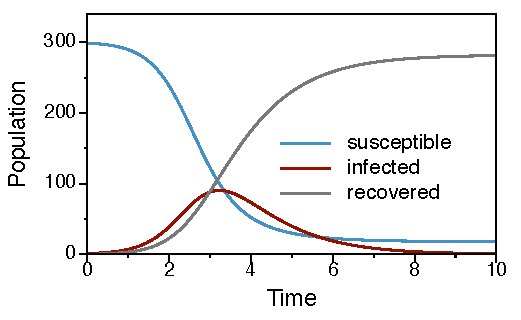
\includegraphics{sir_model.pdf}
\caption{Typical solution of a susceptible-infected-recovered (SIR) model. Parameters: $\alpha = 3$, $\gamma = 1$, $N=300$, $S_0=1$.}
\label{fig:std_sir_model}
\end{center}
\end{figure}
%

The SIR model shows more sophisticated features than the SI model \eqref{eq:si_model}.
To begin with, we analyze the fixed points of the system, i.e. $(S_*,I_*,R_*)$ where
\begin{equation}
\frac{dS_*}{dt} = -\alpha S_*I_* =0 ,\; \;\;
\frac{dI_*}{dt} = \alpha S_*I_* -\gamma I_* =0,\; \;\;
\frac{dR_*}{dt} = \gamma I_* = 0.
\end{equation}
It follows from the last equation that $I_*=0$ at the fixed point, where $S_*$ and $R_*$ can be arbitrary.
Hence, a fixed point is $(S_*,0,R_*)$.

Let us analyze the stability of the fixed point in the early phase of an infection.
Almost all individuals are susceptible and consequently $I_*=N-S_*$.
An outbreak occurs, if and only if $dI/dt >0$ in this phase, i.e.
\begin{equation}\label{eq:prelim_condition}
\frac{dI}{dt}=\alpha S_* (N-S_*) - \gamma (N-S_*)=(N-S_*)(\alpha S_* -\gamma ) >0.
\end{equation}
It follows from \eqref{eq:prelim_condition} that the number of infected grows, if
\begin{equation}\label{eq:prelim_rnod}
\alpha S_* / \gamma >1.
\end{equation}
Equation \eqref{eq:prelim_rnod} is extremely important in epidemiology, because it defines a threshold for the unfolding of an infection spreading process.
We call this fraction the \emph{basic reproduction number} $R_0$.
Recall that $S_* \approx N$ in the fixed point.
Thus it follows that the outbreak condition is
\begin{equation} \label{eq:r0}
R_0 = N \frac{\alpha }{\gamma } >1.
\end{equation}

The basic reproduction number describes the average number of follow-up infections by each infected individual.
It is one of the main goals in epidemiology to bring down the basic reproduction number of a disease below the critical value $R_0=1$.
This is the reason for the implementation of mass vaccination.
As one can immediately see from equation \eqref{eq:r0}, this can be done by reducing the infection rate $\alpha $ or by increasing the immunization rate $\gamma $.
In principle, one could also reduce the size of the initial population $S_*$.
As an example, reducing the infection rate can be done by increasing hygiene standards or appropriate behavior, say wearing warm clothes in winter time to avoid common cold.
The immunization rate can be increased by vaccination.

Let us now focus on the late phase of an SIR-infection.
In contrast to the SI-model of section \ref{sec:si_model} an SIR like outbreak does not necessarily infect the whole population, even if $R_0>1$.
The reason is that there has to be a critical mass of susceptible individuals in order to keep an infection alive (see equation \eqref{eq:prelim_rnod}).
The total number of infected during an infection given by the number of recovered at the end of the infection, since every recovered has to be in the infected state in the first place.
A central measure throughout this work is therefore the \emph{outbreak size} $R_\infty$.

To compute the outbreak size, we consider the second fixed point of \eqref{eq:sir_model}, i.e. the fixed point for $t \rightarrow \infty $.
At this point there are no infected and a fraction of the population is recovered.
Hence the fixed point is $(N-R_\infty , 0, R_\infty )$.
A simple way to obtain the outbreak size $R_\infty $ is to use equations \eqref{eq:sir_model} and compute 
$$
\frac{dS}{dR}=-\frac{\alpha }{\gamma } S 
$$
and separate the variables \cite{Chasnov:2010}.
This yields
$$
\int _{S_*} ^{N-R_\infty} \frac{dS}{S}=-\frac{\alpha }{\gamma } \int _{R_*} ^{R_\infty} dR .
$$
We integrate from the initial condition at $t=0$ to the final condition at $t \rightarrow \infty$, where $S_\infty = N-R_\infty $.
Using that $R_* =0$ at $t=0$ gives 
\begin{equation}\label{eq:transcendental}
R_\infty = S_*-S_* e ^{-\frac{\alpha}{\gamma}R_\infty}.
\end{equation}
This transcendental equation can be solved numerically using a Newton-Raphson technique.
The outbreak size $R_\infty $ only takes finite values for $\alpha / \gamma > 1$.
A solution of equation \eqref{eq:transcendental} is shown in figure \ref{fig:transcendental}
%
\begin{figure}[htbp]
\begin{center}
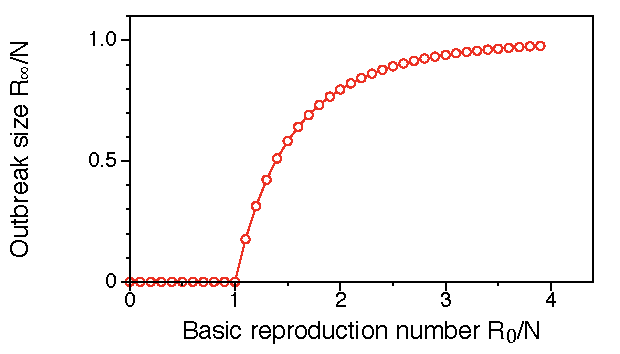
\includegraphics{R_0_R_infty.pdf}
\caption{Relative outbreak size vs. basic reproduction number.
The outbreak size takes finite values only for $R_0/N >1$.
Note that even for supercritical $R_0$ the outbreak size is in general smaller than the total population.
}
\label{fig:transcendental}
\end{center}
\end{figure}

It should be noted that an SIR epidemic is a single event, i.e. it possesses a \emph{characteristic time scale}.
The analysis of the late phase of an epidemic also gives information about these time scales.
Let us consider the second equation of \eqref{eq:sir_model}.
\begin{equation}\label{eq:sir_model_only_i}
\frac{dI}{dt} = \alpha SI -\gamma I
\end{equation}
In the late phase of an SIR-type epidemic, the fraction of infected is small.
Given sufficiently large values of $R_0$, the fraction of recovered is also small in this phase (see figure \ref{fig:transcendental}).
Thus, we neglect the quadratic term in \eqref{eq:sir_model_only_i}.
This gives $\frac{dI}{dt} = -\gamma I $, which has the solution
$$
I(t)=I(0)e^{-\gamma t}.
$$
Hence, the infection decays exponentially for large $t$ and the inverse recovery rate $1/\gamma $ defines the characteristic time of the epidemic.

\subsection{Force of infection}
The model presented in section \ref{sec:sir_model} describes only the very basic behavior of epidemic dynamics, and is therefore a conceptual model.
However, it is one of the main objectives in epidemiology to have an understanding of the exact infection rates in the process.
Infection rates their selves can cause complex infection dynamics.

The term $\alpha I$ used in section \ref{sec:sir_model} is a special, very simple case of an infection rate.
More generally, we have to replace $\alpha I$ by an abstract infection rate $\lambda $ containing more information about the interaction between susceptible and infected individuals \cite{Keeling:2005}.
Thus, the equation for the infected becomes
$$
dI/dt = -\lambda S -\gamma I.
$$
The rate $\lambda $ is called the \emph{force of infection}.
In principle, this parameter can be arbitrarily complex, because it contains detailed information about the mixing properties of the population.
This information could be given as contact networks, demographic contact structures, etc.

In most cases, detailed information about mixing is not available.
Instead, we assume \emph{random mixing} of the population, i.e. every individual can be in contact with every other individual.
This yields a transmission rate \cite{Keeling:2005}
\begin{equation}\label{eq:force_of_infection}
\lambda = \tau n \frac{I}{N}\equiv \beta \frac{I}{N},
\end{equation}
where $\tau $ is the transmission rate, $n$ is the effective contact rate and $I/N$ is the fraction of infectious contacts.
It is therefore reasonable to replace the infection term $\alpha $ in \eqref{eq:sir_model} by $\beta /N$ to explicitly include the force of infection.
Nevertheless, the results presented in section \ref{sec:sir_model} remain qualitatively the same.

Although the force of infection gives a more reasonable description of the infection process, the assumption of random mixing remains inappropriate for many real world systems.
Due to the availability of contact data, the random mixing assumption can be improved in terms of contact networks.
Even if the exact data of an epidemic system is not available, research on complex networks allows us to give more realistic models about mixing.
In the next section, we briefly report important results in complex network research and focus on the interplay between networks and epidemics in section \ref{sec:epidemics_on_networks}.


\section{Complex networks}


\section{Epidemics on networks}\label{sec:epidemics_on_networks}
\subsection{From random mixing to developed structure}

\end{document}

        %\chapter{Outlook}
We give a description of temporal networks later.



        % Part 2
        %\documentclass[openright,twoside,headsepline]{scrbook}
%\usepackage[applemac]{inputenc}
%\usepackage{graphicx,xcolor,hyperref} % obsolete in HU-diss
%\usepackage[round,authoryear]{natbib}
%\setlength\bibhang{2em} 
%
%
%\KOMAoptions{numbers=noenddot}
\usepackage{amsmath,amssymb,amsfonts,amsthm,epigraph,scrpage2}
\usepackage[ngerman,english]{babel}
\definecolor{Cayenne}{rgb}{0.502,0.0,0.0}
\definecolor{Steel}{rgb}{0.4,0.4,0.4}


%\setcounter{secnumdepth}{3} % sub subsections numbering
%\setcounter{tocdepth}{3} % subsubsections inTOC

\usepackage[format=plain,singlelinecheck=false, font={sf,small},labelfont={bf,color=Steel}]{caption}
\DeclareCaptionLabelSeparator{cayenne_period}{\textcolor{Cayenne}{.} }
\captionsetup{labelsep=cayenne_period}

% Colors
\addtokomafont{chapter}{\color{Steel}}
\addtokomafont{section}{\color{Steel}}
\addtokomafont{subsection}{\color{Steel}}
\addtokomafont{subsubsection}{\color{Steel}}
\addtokomafont{paragraph}{\color{Steel}}

\addtokomafont{pagehead}{\color{Steel}}
\renewcommand{\pnumfont}{\color{Steel}} 
\addtokomafont{headsepline}{\color{Steel}} 
\pagestyle{scrheadings} 

%\makeatletter % dot after sections and all below
%\let\std@sect\@sect
%\def\@sect#1#2#3#4#5#6[#7]#8{\std@sect{#1}{#2}{#3}{#4}{#5}{#6}[#7.]{#8\color{Cayenne}{.}}}
%\makeatother

\usepackage[leftcaption]{sidecap} % inner, outer,left,right
\sidecaptionvpos{figure}{t}

% Papiergr��e
%\setlength{\paperwidth}{24cm}
%\setlength{\paperheight}{17cm}
%\recalctypearea
%\usepackage{geometry}

%% Flattersatz
%\usepackage[document]{ragged2e} % Flattersatz
%\setlength{\RaggedRightParindent}{1em} % evtl. parskip


%% Sans Serif
%\usepackage{cmbright}
%\renewcommand{\familydefault}{\sfdefault}
%% Palatino
%\usepackage[sc]{mathpazo}
%\linespread{1.05}         % Palatino needs more leading (space between lines)
%\setkomafont{sectioning}{\normalcolor\bfseries} % Kapitel�berschriften

%%% Kapitel�berschriften: Mit gro�en Zahlen
%\usepackage{titlesec}
%\titleformat{\chapter}[display]
%{\bfseries\Large}
%{ %\Huge\textsc{\chaptertitlename} % f�r das Wort 'Kapitel'
%\hfill\fontsize{120}{70}\selectfont\color{lightgray}\textbf{\thechapter}}
%{-2ex}
%%{\filleft\fontsize{50}{70}\selectfont\scshape} % Kapit�lchen oder...
%{\filleft\fontsize{50}{70}\selectfont\textbf} % ...oder keine Kapit�lchen
%[\vspace{0ex}]
%
%%%% Part�berschriften
%\titleformat{\part}[display]
%{\bfseries\Large}
%{ %\Huge\textsc{\chaptertitlename} % f�r das Wort 'Kapitel'
%\hfill\fontsize{120}{70}\selectfont\color{lightgray}\textbf{\thepart}}
%{-2ex}
%{\filleft\fontsize{50}{70}\selectfont\scshape} % Kapit�lchen oder...
%%{\filleft\fontsize{50}{70}\selectfont\textbf} % ...oder keine Kapit�lchen
%[\vspace{0ex}]


\newcommand{\ER}{Erd\H{o}s-R\'enyi }
\newcommand{\BA}{Barab\'asi-Albert }
\newcommand{\mean}[1]{\left< #1 \right>}
\newcommand{\abs}[1]{\left| #1 \right|}
\newcommand{\norm}[1]{\lVert#1\rVert}
\newcommand{\mat}[1]{\mathbf{#1}}
\newcommand{\tgraph}{\mathcal{G}}

\theoremstyle{definition} % non-italic
\newtheorem{annahme}{Annahme} % braucht amsthm
\newtheorem{definition}{Definition}
\newtheorem{theorem}{Theorem}
\newtheorem{satz}{Satz}
\newtheorem{frage}{Frage}
%\input{watermarks/watermark.tex}
\DeclareMathOperator{\nnz}{nnz}

% + Graphicspath nach begin document

%
%
%
%\begin{document}
%\graphicspath{{/Users/lentz/Documents/GitHub_locals/Thesis/images/}}
%\tableofcontents
%


\chapter{Livestock trade network: Static network analysis}
In this chapter, we address the analysis of static networks, where the focus lies on epidemic spread on networks.
Large amounts of data about different contact structures between a huge amount of subjects became available in the last years.
In the context of epidemics, different types of networks can be obtained.
Concerning infectious diseases of humans, it is unlikely to have the exact contact data of a (sub)-population.
Different methods to extract the contacts structure can be used \citep{Keeling:2005}:
\emph{Contact tracing} is used to determine infection paths under the assumption that every contact has a high probability to cause an infection.
This assumption is justified for highly contagious diseases, such as influenza or sexually transmitted diseases \citep{Rocha_pnas,Rocha_plosbc}.
If more data is available, one can obtain an \emph{infection tracing} network, where every contact definitely caused an infection.
Infection tracing plays an important role for the analysis of HIV spread or food safety \citep{Wilking,Haydon22012003}.
\emph{Diary-based} methods make use of questionnaires to extract contact structures.
The drawback of this method is that the subjects themselves are responsible for the information given and a considerable bias can be present in the data \citep{Visser:2003p784}.
Other diary-based methods make use of legislation in order to guarantee for a sufficient data quality.
An example is the HI-Tier database, which records trade movements of livestock animals and is used for food safety and is a central subject of study in this work \citep{Euro-Lex}.

Based on the amount of available data as quoted above, it is reasonable to model epidemics using a purely topological analysis.
Detailed epidemiology is by far more complex as solving differential equations.
Fine-grained models including large sets of parameters and couplings are needed to model infectious diseases.
A complex example for the transmission of classical swine fever is found in \citep{MartinezLopez:2011db}.
In general, a detailed knowledge about infection probability, contact probability and sensitivity to initial conditions is required to obtain a realistic epidemic model.
Even if this information was available, results could not necessarily be generalized to other systems.

For this reason we restrict the epidemiological aspect of this work to a purely topological analysis of the underlying networks, where detailed data about contact structures is available.
In particular, we focus on a network of pig trade in Germany in the years 2006--2008.
Each node in this network represents an agricultural holding and trade contacts between holdings are represented by directed edges.
(An analogue analysis of a cattle network dataset was published in \citep{Lentz2009}).
This chapter is devoted to a static network analysis of this system and a general topological classification.
In section \ref{sec:temporal_networks} we highlight the effects of a time-resolved treatment of these systems.

\paragraph{Livestock trade dataset\color{Cayenne}{.}}
After the BSE crisis in Europe in 2001, the EU member states established livestock trade movement databases to track potential pathways of pathogen spread.
Since 2001, every holding in Germany is obliged to report every trade movement of live animals (pig, cattle, sheep and goat) to a federal database (\foreignlanguage{ngerman}{Herkunftssicherungs und Informationssystem f�r Tiere} (HIT), \citep{HI-Tier}).
We focus on the trade contacts for pigs.
Trade is recorded in a temporal resolution of 1 day, where the receiving holding and the pre-owner are reported in the database.
In this section we aggregate the trade contacts yielding a static network, where a trade edge is present, if there was at least one trading contact during the observation period.
Our data extract spans the trade within Germany between 01 June 2006 and 31 December 2008.
This yields a static network with $121,223$ nodes and $348,037$ edges.
%This yields a static network with 89,745 nodes and 210,696 edges.

\section{Network analysis}\label{sec:network_analysis}
To begin with, we analyze the livestock trade data according to the measures introduced in section \ref{sec:network_measures}.
\paragraph{Centrality and distances\color{Cayenne}{.}}
Figure \ref{fig:hit_deg_cdf} shows the heavy-tailed degree distribution of the network.
%
\begin{SCfigure}
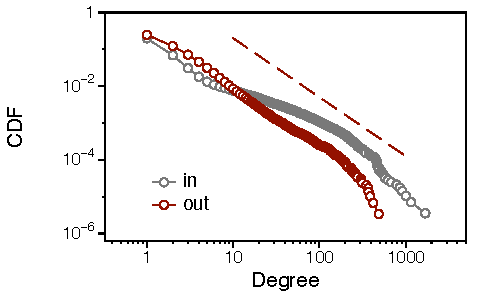
\includegraphics{HIT_Degree_CDF.pdf}
\caption{Degree distribution of the livestock trade network. The out-degree distribution (red circles) is well approximated by a power-law of the form $x^{-1.67}$ (red dashed line).
The in-degree distribution shows a bimodal behavior indicating the presence of large slaughterhouses (grey triangles).
Power law exponent was computed using a maximum likelihood estimator \citep{Clauset:2009}.
}
\label{fig:hit_deg_cdf}
\end{SCfigure}
%

\subsection{Components and ranges}\label{sec:components_ranges}
% all: 121223 nodes
% LWCC: 119858, 2nd: 8
% LSCC: 34693, 2nd: 16
Ignoring the edge direction, the network has a giant component containing almost 99~\% of the nodes. The second largest weakly connected component contains only 8 nodes.
The size of the largest and second largest strongly connected components are 28,6~\% (34,693 nodes) and  0.01~\% (16 nodes), respectively.
Sizes of the next smaller components decrease rapidly.
All in all the network percolates ignoring the direction of links.
Taking into account link directions, the giant component contains a considerable fraction of the network, but is far from the percolation threshold.

The giant strongly connected component has an interesting impact on the distribution of node ranges (and reachabilities) in the network.
Note that the range of a node defines the upper bound for any disease outbreak starting from this very node.
Following equation \eqref{eq:range_def}, we compute the ranges of all nodes and focus for the moment on the \emph{sequence} of these ranges. 
For most sequences of centralities in a network, we would find rather noisy signals.
These signals result in distributions such as the degree distribution in figure \ref{fig:hit_deg_cdf}.
In contrast to most other centrality measures, the range shows a strikingly different behavior.
The sequence of ranges for all nodes in the network is shown in figure \ref{fig:node_range}. 
%
\begin{figure}[htbp]
\begin{center}
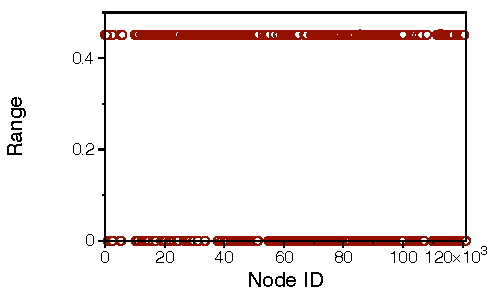
\includegraphics{Node_Range_PVM_100th.pdf}
\caption{Range sequence for all nodes in the livestock trade network.
Every 100th node with range greater than 0 is shown.
}
\label{fig:node_range}
\end{center}
\end{figure}
%
The striking feature here is the \emph{gap} in the distribution: no range in between $7\cdot 10^{-4}$ (87 nodes) and $0.45$ (54693 nodes) is present in the system.
%There is another, smaller gap for values between $0.33$ (29325 nodes) and $0.35$ (31033 nodes).
Consequently, a randomly chosen node can only belong to one of two classes, namely long ranged nodes and short ranged nodes.
A node of the latter class is barely suitable to cause a considerable disease outbreak at all.
Only a node of long range can act as a node for large scale disease outbreaks.
The sizes of the classes in figure \ref{fig:node_range} are as follows: 54,874 nodes belong to the short range and 66,349 nodes to the long range class, respectively.
%91 nodes of the latter are above the second range gap.

For a general network we define the range gap $\Gamma $ as the size of the largest interval, where the range distribution is identically zero \citep{Lentz:2012pre}.
The balance of the distribution around the gap is measured in terms of the variable
\[
b=\frac{N_l-N_s}{N},
\]
where $N=N_l+N_s$ is the number of nodes and $N_l$ and $N_s$ are the numbers of long and short ranged nodes, respectively.
Apparently $b=1$, if all nodes are long ranged and $b=-1$ for only short ranged nodes in the network.
Figure \ref{fig:ER_range_gaps} shows the range gap and balance for directed \ER networks of varying density.
The figure demonstrates, that the size of the range gap and the balance are inherently related to the percolation properties of the system (see section \ref{sec:er_model}).
A significant range gap in combination with equally sized range classes indicates that the system is in a critical state.
The author would like to stress the fact that the combination of range gap and balance is a more general indicator for the critical state than the average degree (see figure \ref{fig:ER_lcc_emergence}, section \ref{sec:er_model}).
This is because the range gap is not subject to any random model assumption.
For the dataset of figure \ref{fig:node_range} we get $\Gamma = 0.45$ and $b=0.095$ indicating that the system is only slightly above the critical point.
Note that for the undirected case, the range of every node is equivalent to the size of the component it belongs to.
Thus, ranges show a rather trivial behavior in the undirected case.
%
\begin{SCfigure}
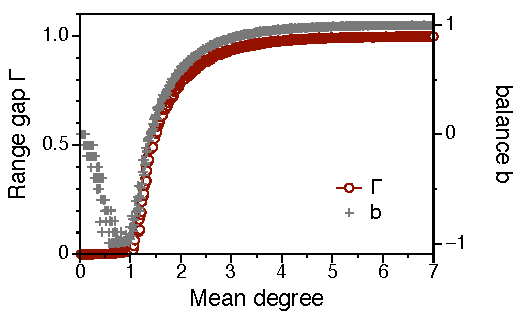
\includegraphics{ER_Range_gap.pdf}
\caption{Range gap $\Gamma $ and balance $b$ vs. mean degree for directed \ER graphs.
Each datapoint is a mean value of 1000 networks. Network size: 1000 nodes.
}
\label{fig:ER_range_gaps}
\end{SCfigure}

The explanation for the strong bi-modality of the range distribution is the existence of a giant strongly connected component (GSCC).
Figure \ref{fig:rangegap_principle} shows a schematic picture of a directed network.
Due to the giant component in the system, all nodes that belong to the GSCC can reach all other nodes in the component plus all nodes that the component is connected to.
%
\begin{figure}[htbp]
\begin{center}
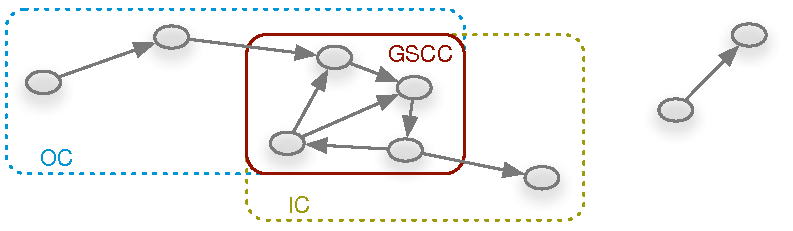
\includegraphics{RangeGap-principle.pdf}
\caption{Schematic structure of a directed network.
In the core region there is the giant strongly connected component (GSCC, red). All nodes reachable from the GSCC form the giant out-component (GOC, yellow) and the nodes with access to the GSCC define the giant in-component (GIC, blue).
The union of GSCC, GIC, GOC and all tendrils is the giant weakly connected component (GWCC) of the network.
Nodes that are not part of the GWCC belong to another component of the network (nodes on the upper right).
}
\label{fig:rangegap_principle}
\end{center}
\end{figure}
%
If there is a path from a node to the GSCC, but the node itself is not on this component, it belongs to the giant in-component (GIC) of the network. 
In analogy, nodes reachable from the GSCC that are themselves not part of the latter, belong to the giant out-component (GOC).
All remaining nodes not belonging to one of the components mentioned above are called tendrils, if they are weakly connected to the GSCC.
The nodes on the upper right (figure \ref{fig:rangegap_principle}) are not even weakly connected to the GSCC and thus belong to another component of the network.

As an explanation for figure \ref{fig:node_range}, the lower bound of the long range node class is formed by the nodes of the GSCC.
Every node that belongs to the long range node class is either on the GSCC or on the GIC.
The low range class is populated by nodes of the GOC, tendrils and nodes of other WCCs.

\subsection{Modules}
The network components analyzed above make a strict requirement to the connectivity between components.
A weaker requirement would be to allow for the existence of only a few edges between components.
The usage of such structures in the context management of disease risk has been suggested in \citep{MartinezLopez2009}.
Structures of this type are called \emph{modules} or \emph{communities}.
The idea of finding modules in networks has been proposed in \citep{Newman06062006}.
In order to detect these structures, a cost function mapping every partition of the network onto a value between 0 and 1 has to be optimized.
\citeauthor{Newman06062006} proposed the modularity $Q$ as an appropriate cost function defined as
\[
Q=\text{(number of edges between communities)}-\text{(expected number of those edges)}
\]
or more formally \citep{Fortunanto2010,Newman06062006}
\begin{equation}\label{eq:modularity}
Q=\frac{1}{2m} \sum _{ij}\left( \mat{A}_{ij}-\frac{k_i k_j}{2m} \right) \delta (c_i,c_j).
\end{equation}
This equation gives the modularity for a network with adjacency matrix $\mat{A}$ and $m$ edges and $k_i$ denotes the degree of the $i$-th node.
%
\begin{SCfigure}
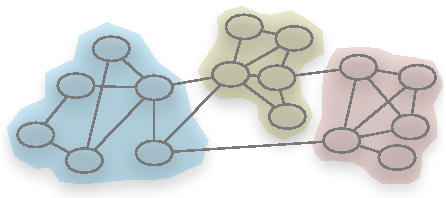
\includegraphics{Module_Prinzip-06diss.pdf}
\caption{The nodes of modular networks are partitioned into modules of high edge density and edges between modules are rare.}
\label{fig:modular_principle}
\end{SCfigure}

%
The partition of the network is given in the Kronecker delta $\delta (c_i,c_j)$, which is 1, if nodes $i$ and $j$ are in the same community and otherwise 0.
Hence, modularity measures the goodness of a particular partition of the network.
$Q\sim 0$ implies that a given partition of a network does not give a significant modular structure.
Its maximum value is $Q=1$ provided that a network has a strong modular partition \emph{and} the latter is known for the computation of $Q$.
Finding best possible partition that maximizes modularity has been shown to be NP-complete \citep{brandes2007}.
However, several approximate methods -- such as simulated annealing \citep{guimera_mod_SA} and greedy algorithms \citep{Clauset_greedy,Newman:fast_algo} -- to maximize modularity have been proposed.
In order to detect community structure in the pig trade network, we analyze the system using the method of \citeauthor{Newman:fast_algo}.
The results presented in this section are published in \citep{Lentz:2011}.
%\footnote{We show results computed for the pig trade data set within observation period 01 june 2006 and 31 december 2008, as in \citep{Lentz:2011}.
%Results remain qualitatively the same for the dataset 01 january 2009 -- march 2010.

Note that we focus on the partition of only the undirected network.
Although the concept of modularity can be generalized to the directed case in a straightforward manner using the definition \citep{Leicht:2008p5144}
\begin{equation}\label{eq:directed_modularity}
Q=\frac{1}{m} \sum _{ij}\left( \mat{A}_{ij}-\frac{k_i ^- k_j ^+}{m} \right) \delta (c_i,c_j),
\end{equation}
there is still ongoing discussion about a systematic bias in this approach \citep{kim2010}.
\citeauthor{kim2010} point out that a straightforward generalization of modularity can not resolve nodes of different in and out degree. 
Hence, nodes of high total degree tend to form communities with their neighborhood regardless of how the links in the neighborhood are directed.

In order to find a partitioning maximizing the modularity function \eqref{eq:modularity}, we use the greedy method proposed in \citep{Clauset_greedy}.
The algorithm was applied to the largest weakly connected component of the network, i.e. $119,858$ nodes.
It finds a partition where 96~\% of all nodes and 98~\% of all edges are assigned to 9 major clusters.
The modularity value for this partition is $Q=0.717$.
After we computation of a suitable network partition, we add the geographical positions of the nodes as further meta information.
The resulting map is shown in figure \ref{fig:D9}.
It should be noted that the community partition was done without spatial information in the first place.
Thus, the figure demonstrates that in this case two nodes of the same community are likely to be geographic neighbors as well.
An explanation for this correlation could be cultural affinity or simply economic reasons, since transport costs scale with geographical distance.

\begin{figure}[htb]
\begin{center}
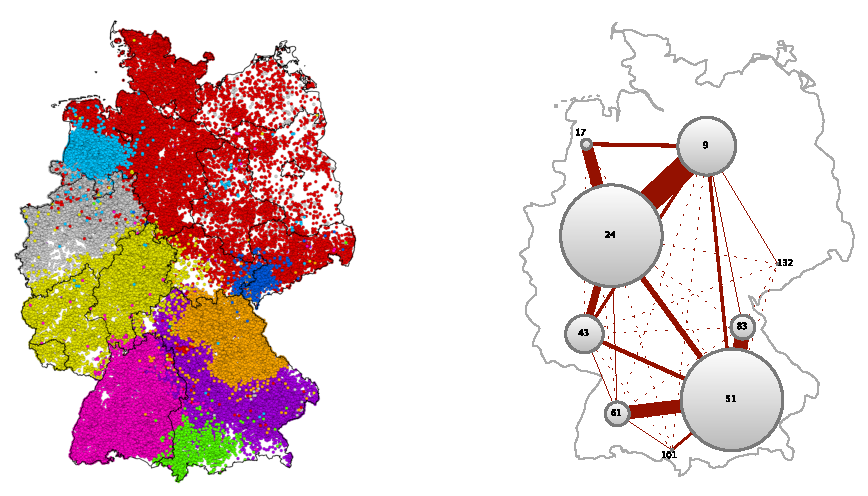
\includegraphics{D9.pdf}
\caption{Geographical embedding of the communities found for the pig trade network (left).
The nine largest (by number of nodes) communities are shown.
The number of edges between the communities and within the communities is shown on the right.
From \citet{Lentz:2011}.
}
\label{fig:D9}
\end{center}
\end{figure}

The right panel of figure \ref{fig:D9} shows the nine largest communities condensed into single nodes, where the size of each node represents the number of edges in the community.
Node numbers are arbitrary IDs given by the used algorithm.
Links between communities are weighted ranging from 6 (dashed lines) to 7251 (massive edge between 24 and 9).
The positions of the nodes approximate the center of mass of the corresponding community on the left panel.

Module detection is a reasonable tool for capturing the large scale structure of networks.
In fact, is has been shown that there is a resolution limit for community detection and the minimum size of the communities depends on the size of the network \citep{SantoFortunato01022007}.
In general, meta information such as the geographical embedding of the network, is needed to gain knowledge about the function of a network out of its structure.

A particular partitioning of a network, however, is not guaranteed to give unambiguous information about the network.
On the contrary, equation \eqref{eq:modularity} is a mapping from a high dimensional partition space to a scalar.
The number of elements in the partition space is given by the \emph{bell number}.
This implies that the number of partitions of a network with 10 nodes is $\sim 10^5$ and it is already $\sim 10^{47}$ for 50 nodes!
Adjacent partitions in the partition space can have huge differences in $Q$ and it is not guaranteed that approximative algorithms are capable to find the global optimum.
Furthermore, a huge number of different partitions can possess the same modularity $Q$.

Although a particular partition should in general be interpreted with caution, we can state that \emph{at least one} partition of a certain value of $Q$ is intrinsic in the system.
I.e. the system is somehow modular, even if the best possible partition might be unknown.
We consider this line of thought in the next section, where we analyze artificial networks with distinctive structural features in order to gain insight into their impact on epidemic processes.

\section{Range \& modules: Spreading potential}\label{sec:PRE}
In this section, we investigate the impact of directionality and modularity of networks on epidemic processes.
Therefore, we use random network models that mimic the desired properties.
To begin with, we derive a system of equations that models an epidemic process as it would take place on the pig trade network of section \ref{sec:network_analysis}.
For this reason, we consider the agricultural holdings as meta-populations and the time scales between trade and infection are separated using a pacing of trade.
All results presented in this section are published in \citep{Lentz:2012pre}.

\subsection{Epidemic model}
In this section, we derive an infection model for agricultural holdings that are considered as meta populations, each holding containing a certain number of animals. 
The coupling between the holdings is given by trade, which appears as transportation of livestock animals (see figure \ref{fig:metapop_scheme}).
The union of all trade couplings is given by a trade network with adjacency matrix $\mat{A}$. 
Since transportation/trade in this sense is a non symmetric process, we focus on \emph{directed networks} in particular.

In each node of the network, a susceptible-infected-recovered (SIR) reaction takes place.
Following section \ref{sec:sir_model}, the infection model for each node $\mu $ in such a system reads
\begin{align}\label{eq:local_sir_only}
\partial _t s_\mu &= -\alpha s_\mu \frac{i_\mu}{n_\mu} \notag \\
\partial _t i_\mu &=  \alpha s_\mu \frac{i_\mu}{n_\mu} - \gamma i_\mu \notag \\
\partial _t r_\mu &= \gamma i_\mu ,
\end{align}
where $n_\mu =s_\mu + i_\mu + r_\mu $ is the total population of node $\mu $ and we use the force of infection $i_\mu / n_\mu $ as suggested in equation \eqref{eq:force_of_infection}.
The \emph{infection status} of node $\mu $ is given by the triple $(s_\mu , i_\mu , r_\mu )$.
Now we add the interactions between the meta populations by introducing a network with adjacency matrix elements $a_{\mu \nu }$.

The total \emph{outflow} from node $\mu $ is given by its degree $\sum _\nu a_{\mu \nu }$ and divides into
\[
f_\mu ^- =  \frac{s_\mu }{n_\mu} \sum _\nu a_{\mu \nu } + \frac{i_\mu }{n_\mu} \sum _\nu a_{\mu \nu }+ \frac{r_\mu }{n_\mu} \sum _\nu a_{\mu \nu }
\]
according to the infection status of the node.
The \emph{inflow} of each node depends on the infection status of its predecessors in the network, i.e.
\[
f_\mu ^+ =\sum _\nu a^T _{\mu \nu }\frac{s_\nu }{n_\nu } + \sum _\nu a^T _{\mu \nu }\frac{i_\nu }{n_\nu } + \sum _\nu a^T _{\mu \nu }\frac{r_\nu }{n_\nu },
\]
where $\sum _\nu a^T _{\mu \nu }=\sum _\nu a _{\nu \mu }$ is the in degree of node $\mu $.
We add the respective contributions of inflow and outflow to equations \eqref{eq:local_sir_only} and get
%
\begin{align}
\partial _t s_\mu &= -\alpha s_\mu \frac{i_\mu}{n_\mu} + \sum _\nu a^T _{\mu \nu} \frac{s_\nu }{n_\nu } - \frac{s_\mu }{n_\mu }  \sum _\nu a_{\mu \nu} \notag \\
\partial _t i_\mu &=  \alpha s_\mu \frac{i_\mu}{n_\mu} + \sum _\nu a^T _{\mu \nu} \frac{i_\nu }{n_\nu  } - \frac{i_\mu }{n_\mu  }  \sum _\nu a_{\mu \nu} -\gamma i_\mu \notag \\
\partial _t r_\mu &= \sum _\nu a^T _{\mu \nu} \frac{r_\nu }{n_\nu } - \frac{r_\mu }{n_\mu }  \sum _\nu a_{\mu \nu} +\gamma i_\mu .
\label{eq:sir_indices_pre} 
\end{align}
%
Regarding this equation system, we have to address the impact of directionality, i.e. the non-symmetry of the adjacency matrix.
Considering the coupling term in equations \eqref{eq:sir_indices_pre}, we have to make sure that the population of each node remains constant, i.e. $f_\mu ^- = f_\mu ^+$.
Using that $\frac{s_\nu}{n_\nu} +\frac{i_\nu}{n_\nu} +\frac{r_\nu}{n_\nu} =1$ this is equivalent to the condition
\[
\sum _\nu (a_{\nu \mu }-a_{\mu \nu})=0.
\]
In undirected networks, this condition is always satisfied.
In directed networks, however, the condition implies that each node in the network has the same in and out degree, respectively.
This does not hold in the general case, so that the total flow of node $\mu $ is
\[
\sum _\nu (a_{\nu \mu }-a_{\mu \nu})= f_\mu ^+ -f_\mu ^- \equiv f_\mu \neq 0 ,
\]
i.e. the difference between in-degree and out-degree.
This difference is distributed over the infection status of the respective node so that
\[
f_\mu =\frac{s_\mu }{n_\mu }f_\mu ^s +\frac{i_\mu }{n_\mu }f_\mu ^i +\frac{r_\mu }{n_\mu }f_\mu ^r .
\]
It follows that in the case of a directed network, we have to add a birth/death process in each node to keep the total population constant.
Hence, the infection model becomes
%
\begin{align}
\partial _t s_\mu &= -\alpha s_\mu \frac{i_\mu}{n_\mu} + \sum _\nu a^T _{\mu \nu} \frac{s_\nu }{n_\nu } - \frac{s_\mu }{n_\mu }  \sum _\nu a_{\mu \nu} -\frac{s_\mu }{n_\mu } f^s _\mu \notag \\
\partial _t i_\mu &=  \alpha s_\mu \frac{i_\mu}{n_\mu} + \sum _\nu a^T _{\mu \nu} \frac{i_\nu }{n_\nu  } - \frac{i_\mu }{n_\mu  }  \sum _\nu a_{\mu \nu} -\gamma i_\mu -\frac{i_\mu }{n_\mu } f^i _\mu \notag \\
\partial _t r_\mu &= \sum _\nu a^T _{\mu \nu} \frac{r_\nu }{n_\nu } - \frac{r_\mu }{n_\mu }  \sum _\nu a_{\mu \nu} +\gamma i_\mu -\frac{r_\mu }{n_\mu } f^r _\mu .
\label{eq:sir_indices_with_flow_correction} 
\end{align}
%
In analogy to section \ref{sec:network_matrices}, we define the Laplace Matrix $\mat{L}$ with elements
\begin{equation}\label{eq:sir_laplace}
l_{\mu \nu} = a^T _{\mu \nu } - \delta _{\mu \nu }\sum _\sigma a_{\mu \sigma } .
\end{equation}
Using vector notation, the status of the whole network is given by the respective vectors $\mat{S}$, $\mat{I}$ and $\mat{R}$.
Lowercase letters refer to normalized variables, i. e. the elements of $\mat{s}$ are $s_\mu / n_\mu $.
the system \eqref{eq:sir_indices_with_flow_correction} now reads
\begin{align}\label{eq:sir_no_pacing}
\partial _t \mat{S} &=\mat{L}\mat{s}- \mathrm{diag} (\mat{s}\mat{F}_s)-\alpha \; \mathrm{diag}(\mat{S}\mat{i}) \nonumber \\
\partial _t \mat{I} &=\mat{L}\mat{i}- \mathrm{diag} (\mat{s}\mat{F}_i)-\alpha \; \mathrm{diag}(\mat{S}\mat{i}) -\gamma \mat{I} \nonumber \\
\partial _t \mat{S} &=\mat{L}\mat{r}- \mathrm{diag} (\mat{r}\mat{F}_r) +\gamma \mat{I} .
\end{align}
This system models an SIR-type epidemic on a meta population which is connected by a network structure given by the Laplacian $\mat{L}$.
In \eqref{eq:sir_no_pacing}, $\mathrm{diag} (\mat{x} \mat{y})$ denotes the main diagonal of the outer product of vectors $\mat{x}$ and $\mat{y}$.

Still, the infection time scale is the same as the trade time scale in \eqref{eq:sir_no_pacing}.
In order to separate these time scales, we modify the Laplacian \eqref{eq:sir_laplace} and define a \emph{paced Laplacian}
\begin{equation}\label{eq:new_laplacian}
\mathcal{L}(\tau )=\mat{L} \sum _{n=0} ^\infty  \delta (t-n\tau )
\end{equation}
with pacing frequency $\tau $.
Thus, we obtain the requested model replacing the Laplacian in \eqref{eq:sir_no_pacing} by its paced counterpart.
Finally , we use the following outbreak model:
%
\begin{align}\label{eq:sir_with_pacing}
\partial _t \mat{S} &=\mathcal{L}(\tau )\mat{s}- \mathrm{diag} (\mat{s}\mat{F}_s)-\alpha \; \mathrm{diag}(\mat{S}\mat{i}) \nonumber \\
\partial _t \mat{I} &=\mathcal{L}(\tau )\mat{i}- \mathrm{diag} (\mat{s}\mat{F}_i)-\alpha \; \mathrm{diag}(\mat{S}\mat{i}) -\gamma \mat{I} \nonumber \\
\partial _t \mat{S} &=\mathcal{L}(\tau )\mat{r}- \mathrm{diag} (\mat{r}\mat{F}_r) +\gamma \mat{I} .
\end{align}
%
In order to analyze the impact of characteristic topological features -- in particular modularity and directionality -- on disease dynamics, we solve equations \eqref{eq:sir_with_pacing} numerically for different computer-generated networks with the desired properties.

\subsection{Computer-generated networks}\label{sec:computer-gen-networks}
In this section we describe how networks with varying directionality and modularity can be generated on a computer.
Although generating a sequence of graphs with a certain directionality is straightforward, we have to discuss how to quantify this property.
Before we generate networks of a desired modularity, we address restrictions in the maximum value of $Q$.

\paragraph{Networks of varying directionality\color{Cayenne}{.}}
The directionality of a given network is related to its fraction of bidirectional links.
In principle, the strength of direction could be measured this way.
It has been shown, however, that this measure would yield finite values even for purely random networks \citep{Garlaschelli2004}.
Therefore, \citeauthor{Garlaschelli2004} introduced the measure of \emph{link reciprocity} $\rho $ of a given network with $N$ nodes and adjacency matrix $\mat{A}$ as
\begin{equation}\label{eq:link_reciprocity}
\rho =\frac{\sum _{i\neq j} (a_{ij}-\bar{a})(a^T _{ij}-\bar{a})}{\sum _{i\neq j} (a_{ij}-\bar{a})^2}.
\end{equation}
The edge density is denoted as $\bar{a}=\sum _{ij} a_{ij}/(N(N-1))$.
In fact, equation \eqref{eq:link_reciprocity} is the correlation between an adjacency matrix and its transposed.
Reciprocity $\rho =1$ for undirected networks, whereas $\rho \approx 0 $ for directed random graphs.
In the latter case the fraction of bidirectional links would take finite values, since some bidirectional links are taken by chance.

To investigate the impact of directionality on disease dynamics, we generate random networks with different values of $\rho $ and solve the system \eqref{eq:sir_with_pacing} on these topologies.
The networks are generated as follows:
1. generate an undirected \ER network, 2. replace all edges by bidirectional directed edge pairs and 3. remove one edge of the bidirectional edge pair with probability $q$.
Consequently, the probability that an edge pair is connected by an undirected (bidirectional) edge is $p_\mathrm{rev} = 1-q$.
The link reciprocity of the generated network can directly be computed using equation \eqref{eq:link_reciprocity}.
We have to point out that this analysis focuses on \ER networks.
Other network types are possible as well, but would add more complexity to the analysis.  

\paragraph{Modular networks\color{Cayenne}{.}}
Following \citeauthor{Newman:2004}, a modular network can be realized as a union of independent subgraphs, that are afterwards sparsely connected \citep{Newman:2004}.
In this work, we use random networks with fixed node number $N$ and edge probability $p$ as subgraphs.
The connection of subgraphs is achieved by by placing edges between them with probability $p_\mathrm{out}$.
Varying $p_\mathrm{out}$ allows for an adjustment of the modularity $Q$, which is computed using equation \eqref{eq:directed_modularity}.

It should be noted that a sufficient number of subgraphs is necessary to obtain large values of $Q$.
We found an analytic approximation for the maximum possible modularity by maximizing equation \eqref{eq:modularity} (or \eqref{eq:directed_modularity}, respectively) for different module numbers. 
For a network of $n$ modules the maximum modularity is
\begin{equation}\label{eq:Q_max}
Q_\mathrm{max}=1-\frac{1}{n}.
\end{equation}
Derivation sketch: given a modular network with adjacency matrix $\mat{A}$, there is always a relabeling of indices $\mat{P}$ so that $\mat{A}'=\mat{P}\mat{A}\mat{P}^{-1}$ is block diagonal.
The maximum modularity can be derived from the blocks of $\mat{A}'$, since the graphs of $\mat{A}'$ and $\mat{A}$ are isomorphic.
A full derivation of \eqref{eq:Q_max} is given in Appendix \ref{sec:maximum_modularity_subgraphs}.

\subsection{Impact of directionality}\label{sec:impact_directionality}
We solve the system \eqref{eq:sir_with_pacing} on a sequence of networks as generated according to the previous section.
For the rest of this work, we keep the following parameters constant:
The infection parameters are $\alpha =3$, $\gamma = 1$, $\tau =21$.
The initial infection status of all nodes are $(s_\mu (0),i_\mu (0),r_\mu (0))=(300,0,0)$.
As initial conditions, we choose the node with longest range to avoid trivial solutions and its initial state is $(299,1,0)$.
Figure \ref{fig:typical_trajectory} shows a typical solution of the system on a random network.

\begin{SCfigure}
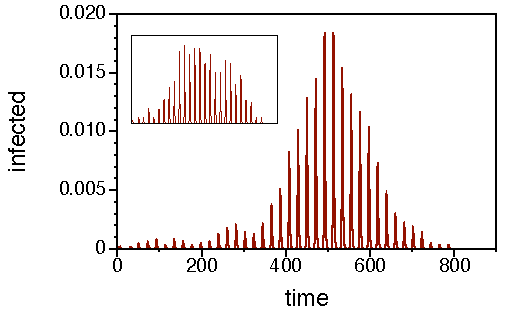
\includegraphics{Typical_Trajectory.pdf}
\caption{Typical infection curve $\sum _\nu i_\nu (t)$ of a solution of equation \eqref{eq:sir_with_pacing}.
The ratio of $1/\tau $ and $\gamma $ results in a comb shape of the infection curve.
Inset shows the more noisy infection curve of a critical network.
Networks: \ER network with 2000 nodes, $p=0.05$, $p_\mathrm{rev}=0.5$ (inset: $p=0.001$, $p_\mathrm{rev}=0.01$).
From \citep{Lentz:2012pre}.
}
\label{fig:typical_trajectory}
\end{SCfigure}

Although the choice of parameters seems a bit arbitrary in the first place, the qualitative behavior of the system depends only weakly on the exact parameter values \citep{Lentz:2012pre}.
We have seen in section \ref{sec:sir_model} that the outbreak condition \eqref{eq:r0} determines whether an outbreak occurs at all.
Above threshold, SIR-type outbreaks show quasi similar behavior.
That is why the fraction $\alpha / \gamma $ in equations \eqref{eq:sir_with_pacing} is of minor importance as long as $\alpha / \gamma >1$.
In addition to that, the characteristic time scale of an SIR infection is given by $1/\gamma $ (see equation \eqref{eq:sir_characteristic_time_scale_gamma}).
If the pacing of the network coupling $\tau $ is too slow, a local infection dies out before it can be moved to the next node.
Therefore, we choose $\tau $ and $\gamma $ so that an infection can spread along the network.
An analysis of the outbreak dynamics in the $(\tau \gamma)$ parameter space is given in \citep{Lentz:2012pre}.

After integrating the system \eqref{eq:sir_with_pacing} on computer generated networks, we compute the final size of epidemic (see section \ref{sec:sir_model})
\[
R_\infty = \lim _{t\rightarrow \infty } \sum _\nu r_\nu (t),
\]
which is normalized by the population size $P$ to yield the outbreak size
\begin{equation}\label{eq:pre_outbreak_size}
r_\infty =\frac{R_\infty}{P}.
\end{equation}
Figure \ref{fig:outbreaksize_vs_rec_ER} shows the outbreak size for \ER networks with different values of link reciprocity.
The plot shows networks of different densities determined by the edge occupation probability $p$.
Note that $p$ corresponds to the edge density before edge removal as described in section \ref{sec:computer-gen-networks}.
Hence, the edge density is further reduced for smaller values of $\rho $.
%
\begin{figure}[htb]
\begin{center}
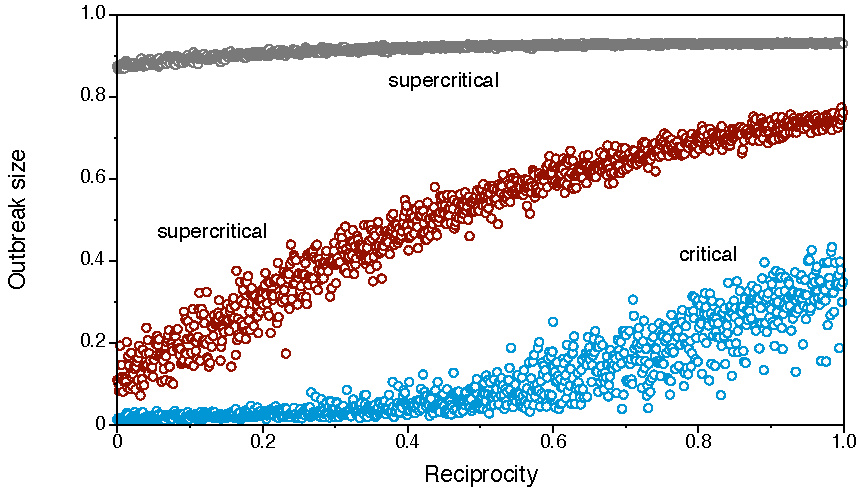
\includegraphics{Outbreaksize_vs_rec_ER.pdf}
\caption{Effect of directionality for an SIR outbreak on a random network.
Each point corresponds to one outbreak simulation on one network.
All networks have 2000 nodes.
Initial network densities: grey: $p=0.003$, red: $p=0.001$, blue: $p = 0.000625$.
From \citep{Lentz:2012pre}.
}
\label{fig:outbreaksize_vs_rec_ER}
\end{center}
\end{figure}

Grey points in figure \ref{fig:outbreaksize_vs_rec_ER} represent outbreaks in rather dense ($p=0.003$) networks.
This density is significantly larger than the percolation threshold of the network, which is $p_c=0.0005$.
Thus, the networks are clearly supercritical.
The figure demonstrates that the outbreak size is almost constant for all values of $\rho $, indicating that the high link density of the network is not affected by a removal of some bidirectional links.
The red points also represent outbreaks on supercritical networks, but the densities of the networks are only slightly above the critical point.
As a consequence, the outbreak size is more sensitive to changes of reciprocity.
The outbreak size range from $0.1$ to $0.8$ in this case.
The density of the blue outbreaks correspond to networks with initial density $p=0.000625$.
Consequently, the density is approximately $0.0005=p_c$ for $\rho =0.5 $.
This implies, that the network undergoes a phase transition for $\rho =0.5$.
As shown in the figure, the outbreak size depends on the link reciprocity only in the supercritical regime.

The findings of figure \ref{fig:outbreaksize_vs_rec_ER} demonstrate, that the structure of the underlying network affects the outbreak size. In particular, critical networks show a strong sensitivity to changes in directionality.
Nevertheless, it can be shown that the effect behind the results in figure \ref{fig:outbreaksize_vs_rec_ER} is not due to mixing of the population, but can in fact be explained by purely topological arguments \citep{Lentz:2012pre}.
This is shown by comparing the range of the initially infected node with the actual size of the disease outbreak.
A deviation between the two would indicate that back-mixing of recovered into the population is responsible for a decrease in outbreak size, since recovered do not contribute to the infection process, but can act as infection firewalls.

\subsection{Impact of modularity}\label{sec:impact_of_modularity}
Before we study the impact of modularity, we define the \emph{time of outbreak peak} in order to quantify the time period of the main epidemic.
The peak time of the epidemic is defined as the time, that divides the infection curve into two equal areas, i.e. the ``median'' of the infection curve.
Since this corresponds to the time, where half of the final infection size is reached.
It follows from the SIR model \eqref{eq:sir_model} that the time of infection peak can also be computed using
\begin{equation}\label{eq:pre_time_of_infection_peak}
t: i(t)= R_\infty /2 .
\end{equation}
Using the term ``median'', the number of recovered is -- up to a constant -- the ``cumulative distribution'' of the infection curve, i.e $dR/dt=\gamma I$.

As in the previous section, we compute the outbreak sizes and the infection peak times for networks of different modularity generated according to section \ref{sec:computer-gen-networks}.
For each outbreak, we compute the outbreak size $r_\infty $ following \eqref{eq:pre_outbreak_size} and the time of infection peak as defined in \eqref{eq:pre_time_of_infection_peak}.
The results are shown in figure \ref{fig:time_rinfty_vs_mod}.
%
\begin{figure}[htb]
\begin{center}
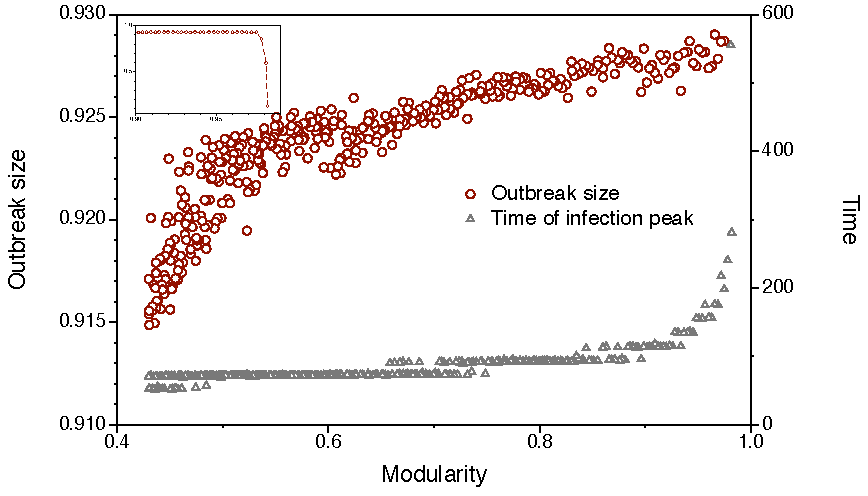
\includegraphics{Outbreaksieandtime_vs_Q}
\caption{Impact of modularity $Q$ on the outbreak size $r_\infty $. The outbreak size (red circles) is affected by an increase of modularity, although the effect is rather weak.
The inset shows the disintegration of the network resulting in a drop of the outbreak size for very large values of $Q$.
Grey triangles demonstrate that increasing modularity can cause significant delays of the infection peak.}
\label{fig:time_rinfty_vs_mod}
\end{center}
\end{figure}

As the figure demonstrates, the size of infection increases with modularity (red circles).
This can be explained by the distribution of recovered and infected:
In the early phase the epidemic is localized in the initial module, while it is unlikely that other modules become infected in the first place.
Modules have a high link density by definition so that an infection is likely to infect large parts of the initial module in the early phase.
In the moment when a path is accessible to another module, the new module is likely to comprise of a large number of susceptible population.
Therefore, the recovered subpopulation cannot act as a firewall against infection spread.

It should be noted that the effect is marginal over a wide range of modularity.
The inset shows that a very high modularity causes a significant drop of the outbreak size, since the network disintegrates into disconnected components in this limit.
In contrast to the effect discussed above, the drop of outbreak size in the limit $Q\rightarrow 1$ is a purely topological one \citep{Lentz:2012pre}.
This can be shown with the same arguments as in section \ref{sec:impact_directionality}.

In addition to that, figure \ref{fig:time_rinfty_vs_mod} shows the time of infection peak for different modularities (grey triangles).
For small and intermediate values of $Q$, we observe a slight delay of the outbreak peak.
The quantified behavior of the plot stems from the pacing $\tau $ of the network.
The main finding of the figure is that large values of modularity cause a significant delay of the outbreak peak.
This knowledge could be useful for the implementation of counter measures, such as vaccination strategies.
Consequently, there is more time to react in high modular networks.


\subsection{Impact of reciprocity in modular networks}
In this section, we focus on modular networks with varying link reciprocity, i.e. we combine the properties studied in sections \ref{sec:impact_directionality} and \ref{sec:impact_of_modularity}.
We generate a number of modular networks and change their link reciprocity afterwards.
Solving the infection model \eqref{eq:sir_model} on these topologies gives outbreak sizes for different reciprocities.
The results are shown in figure \ref{fig:outbreak_vs_rec_modular}.
%
\begin{figure}[htb]
\begin{center}
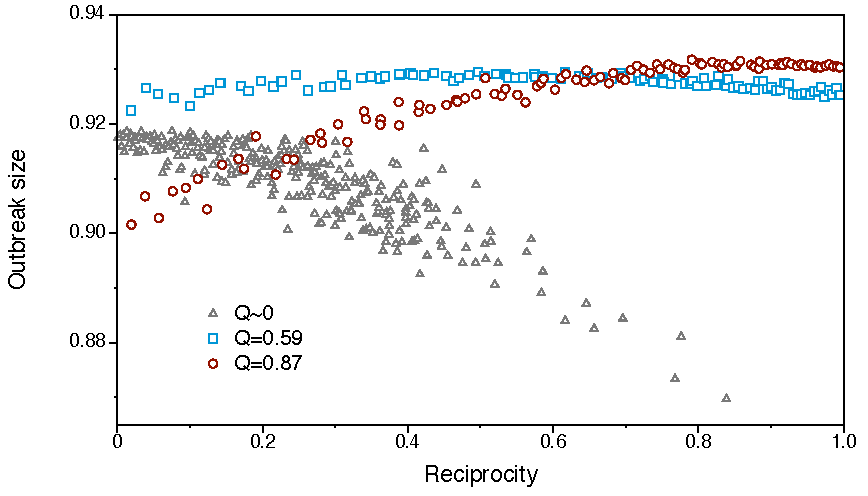
\includegraphics{Outbreaksize_vs_rec_modular.pdf}
\caption{Outbreak size vs. link reciprocity for modular networks.
Changing reciprocity in intermediate modular networks (blue squares) does not affect the outbreak size significantly.
Highly modular networks (red circles) act as isolated modules and show a behavior similar to that of figure \ref{fig:outbreaksize_vs_rec_ER}.
The correlation between outbreak size and reciprocity is reversed for very low modular networks (grey triangles)}
\label{fig:outbreak_vs_rec_modular}
\end{center}
\end{figure}

The red circles in figure \ref{fig:outbreak_vs_rec_modular} represent networks with $Q=0.87$, i.e. highly modular networks.
The outbreak size shows a behavior comparable to that of the supercritical \ER graphs in figure \ref{fig:outbreaksize_vs_rec_ER}.
This provides evidence for the hypothesis that the modules of highly modular networks act as isolated subgraphs.
For networks of intermediate modularity ($Q=0.59$, blue squares), there is almost no correlation between outbreak size and link reciprocity.

Interestingly, the correlation between outbreak size and link reciprocity becomes even negative for networks of very low modularity ($Q\sim 0$, grey triangles).
Grey triangles should not be confused with random networks.
In fact, they are generated as modular networks, but with very high inter-module edge probabilities $p_\mathrm{out}$, i.e. they possess an internal structure, but this structure is not resolved by the modularity any more.
This can can be seen as a limit $Q\searrow 0$.
A possible explanation for the counter-intuitive behavior of low modular networks is that there is a high probability that an infected subpopulation $M$ is highly connected to the module $M_0$ where the infection originated from.
As a matter of fact, the module $M_0$ is in an ``older'' infection state, i.e. it is dominated by recovered population.
Consequently, the effective number of susceptible population is decreased for this infection path and the spreading range is reduced.

\paragraph{Conclusion of the section\color{Cayenne}{.}}
The German pig trade network was analyzed in terms of static network measures.
Our main observations are the following:
First off, the system possesses a heavy-tailed degree distribution (figure \ref{fig:hit_deg_cdf}) indicating that the system is heterogenous and be vulnerable to epidemics (see section \ref{sec:epi_networks}).
Second, the network components and the distribution of ranges result in a node classification into either long range or short range nodes.
Any ranking of nodes according to their potential of disease spread is reduced to the class membership of the nodes in this context.
In addition to that, the balance $b$ of the range distribution provides evidence that the system considered here is in a critical state ($b=0.069$, see also figure \ref{fig:ER_range_gaps}).
The directionality of the network is inherently related to the gap seen in the range distribution.
An undirected network would not show a two class distribution.
Third, the network under consideration can be partitioned into modules, i.e. relatively densely connected subgraphs.
By adding meta-information (in this case geographical information) to the network partition, we found a reasonable partition into compact geographical regions (see figure \ref{fig:D9}).
The large scale trade structure of the system can be revealed this way.

Finally, the observations above raise two questions for the context of epidemics on networks:
1. how do link directions affect an epidemic outbreak? and
2. given a network is somehow modular, does this have any impact on disease dynamics?
In order to answer these questions, we generated random networks that allow for  a variation of the desired properties -- directionality and modularity -- and solved an infection model tailor made for a livestock trade network on these topologies.

Our main findings are: 1. Modularity can cause a significant delay of an outbreak, 2. stronger link directionality generally reduces the outbreak size, but in special topologies the effect can also be reversed.



%
%\bibliographystyle{apalike}
%\bibliography{/Users/lentz/Documents/GitHub_locals/Thesis/bibliography.bib}
%\end{document}

       
        % Part 3
        \chapter{Temporal network analysis -- Case study: Livestock trade network}\label{sec:temporal_networks}
The previous chapter has demonstrated that network analysis provides a deep insight into the processes behind epidemic spreading.
Given a sufficient amount of data, a contact network is capable to capture all possible infection pathways in the system.
The potential of static network analysis lies in the huge toolbox of methods that has been developed in the last decades.
As depicted in Section~\ref{sec:network_theory}, there exist conclusive definitions for both their large scale topological features and local centrality measures allowing for node rankings.

Nevertheless, the concept of static networks neglects temporal variations in the system, i.e. the edges of a particular network are not necessarily present at all times.
Networks showing a sparse and heterogenous temporal occurrence of edges are said to show \emph{bursty} behavior.
This chapter addresses some of the conceptional problems owing to bursty links occurence, the most central one being the \emph{causality} of paths.
Section~\ref{sec:Plos} focusses on the computational analysis of the full temporal representation of the network analyzed in Section~\ref{sec:network_analysis}.
In Section~\ref{sec:PRL}, we present a novel formalism mapping the causality of temporal networks onto a mathematical graph.

\section{Introduction}
To begin with, we highlight the most fundamental difference between static and temporal networks.
In particular, we compare the static to the temporal representation of the system.
Figure~\ref{fig:temporal_network_principle} shows a temporal network and its aggregated graph.
%
\begin{figure}[htb]
\begin{center}
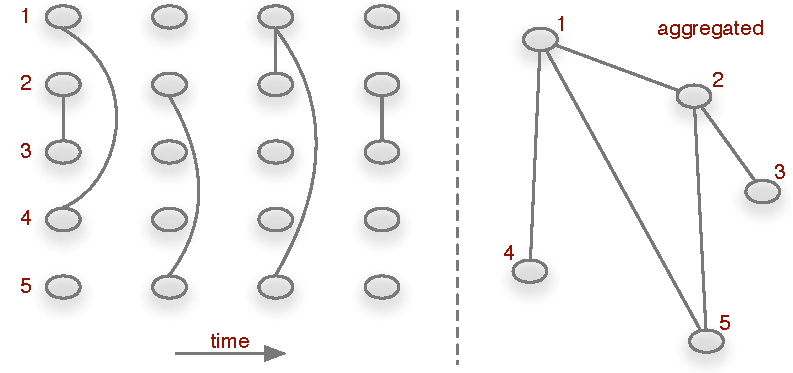
\includegraphics{Temporal_Network_Principle.pdf}
\caption{%
Role of causality in a temporal network with $5$ nodes and $4$ snapshots.
The left panel shows snapshots of the system at different times and the right panel shows the corresponding aggregated network.
Although there is a path from node $3$ to $4$ (and vice versa) in the aggregated network (right panel), there is no causal path between $3$ and $4$ in the temporal network (left panel).
}
\label{fig:temporal_network_principle}
\end{center}
\end{figure}
%
Although the edges of the temporal network are present also in the aggregated graph, the existence of paths of length greater than one is not as obvious.
The aggregated graph (right panel in Figure~\ref{fig:temporal_network_principle}) suggests that the network is connected, i.e. there is a path between every node pair.
As an example, there are two different paths from node $3$ to $4$ in the aggregated system.
However, this does not hold for the temporal view of the system.
Consequently, paths in an aggregated graph of a temporal network have to be treated with care.

Before we give a formal definition of temporal networks, we briefly discuss the different terms used for temporal networks in the literature.
Hereby, we have to distinguish between temporal networks in the sense above and other systems, which have a different focus.

\paragraph{Disambiguation\color{Cayenne}{.}}
Since the analysis of temporal networks is an interdisciplinary field, there is still no consistent designation for what we refer to as \emph{temporal networks} \citep{Holme_review}.
Different phrases, such as temporal graphs, dynamic graphs, dynamic networks are used in the literature.
In addition to that, there are other classes of networks seeming to be related to temporal networks, i.e. adaptive networks, growing networks, evolving graphs.
The analysis of the latter has a strong focus on network growth, i.e. the process behind the evolution of static networks.
A central question for these systems is what is the fundamental process that has formed the network.
An example is the \BA network, where the underlying process is a rich-get-richer principle that results in a scale free degree distribution.
The striking difference between growing networks and temporal networks is that the snapshots of a temporal network can in principle be arbitrary.
Correlations between two snapshots of the system (if any) could be over arbitrary periods of time.
We prefer the term temporal network, since \emph{temporal} is not so easily confused with dynamic systems.
Furthermore, the systems under consideration are not mathematical graphs; therefore, we use the more general term \emph{network}.

\subsection{Formal definition}
A temporal network $\mathcal{G}=(V,\mathcal{E},T)$ consists of a set of nodes $V$ and a set of edges $\mathcal{E}$, where each edge in $\mathcal{E}$ is given by a triple $(u,v,t)$ and connects nodes $u$ and $v$ at time $t\in T$.
$T$ is the observation period of $\mathcal{G}$, where $T\subset \mathbb{N}^+$ for time discrete systems and $T\subset \mathbb{R}^+$ for continuous systems%
\footnote{%
In this thesis, we focus on time discrete systems, since a continuous time process can be approximated by a discrete one by choosing an appropriately small increment.
Furthermore, edge weights and a latency functions for edge traversal could be added to the definition \citep{Casteights_review}.
This is, however, beyond the scope of this thesis.
}.
Using discrete time steps, a temporal network can be represented as a sequence of static snapshots, i.e. $\mathcal{G}=G_1,\dots ,G_T$.
The aggregated graph $G=(V,E)$ of a temporal network simply ignores the occurrence times of the edges in $\mathcal{E}$ and the set of nodes $V$ is the same in both representations.
%
In analogy to static networks, we denote the \emph{transitive closure} of $\mathcal{G}=(V,\mathcal{E},T)$ by $\mathcal{G}^*=(V,\mathcal{E}^*,T)$, where $\mathcal{E}^*$ contains an edge $(u,v,t)$, wherever there is a causal path from node $u$ to $v$ arriving at time $t$ and having started at some time $t_0<t$.
%
Following \citep{Casteights_review}, the \emph{horizon} $\mathcal{H}$ of node $u$ is defined by the set
\begin{equation}\label{eq:temporal_horizon}
\mathcal{H}_u = \left\{ v: \exists \; u\rightsquigarrow v  \right\},
\end{equation}
where $ u\rightsquigarrow v $ means that there is a causal path from node $u$ to $v$.

\subsection{Viewpoints and implementation}\label{sec:tvg_viewpoints}
As in the case of static networks, temporal networks can be interpreted and implemented in different ways \citep{Casteights_review}.
A brief report of different implementations of static networks is given in Appendix~\ref{sec:implementation}.
Besides the adjacency matrix, edge lists and adjacency lists are appropriate network representations.
Considering a temporal network as a sequence of static networks (called snapshots or graphlets) can be seen as a \emph{graph centric} view on the system.
It is the analogue of the adjacency matrix in static networks.
More formally, a temporal network $\mathcal{G}$ can be represented by a sequence of adjacency matrices
\begin{equation}\label{eq:AdMatrixSequence}
\mathcal{A}=\mat{A}_1,\dots ,\mat{A}_T,
\end{equation}
where $T$ is the observation time and the increment is the temporal resolution.

In analogy to the edge lists of static networks (see Appendix~\ref{sec:implementation}), an \emph{edge centric} view on a temporal network is represented by an edge set respecting the occurrence times of the edges.
Let $\mathcal{G}=(V,\mathcal{E})$ be a temporal network.
Than the set of edges $\mathcal{E}$ is represented by a sequence of triples
\begin{equation*}%\label{eq:temporal_edges}
\mathcal{E}=(u_1,v_1,t_1),(u_1,v_1,t_2),(u_2,v_2,t_2),\dots \;.
\end{equation*}
Alternatively the set of edges can be expressed in the form
\[
\mathcal{I}((u_1,v_1))=t_1,t_2,\dots \; ,
\]
where $\mathcal{I}$ is called edge presence function.
This point of view is particularly convenient for the time randomization of temporal networks that we will use in Section~\ref{sec:randomized_models_tvg}.

Finally, a \emph{node centric} view of a temporal network considers the neighborhood $\mathcal{N}$ of a node $v$ over time, i.e. $\mathcal{N}(v,t)$.
This view is the counterpart of the adjacency list in static networks (see Appendix~\ref{sec:implementation}).
The temporal degree of each node immediately follows from $d(v,t)=\abs{\mathcal{N}(v,t)}$.
The edge centric and node centric network view is considered as a microscopic perspective, while the graph centric view provides a macroscopic perspective.

We make use of microscopic perspective implicitly in computer implementations as in Section~\ref{sec:Plos}.
Furthermore, we focus on the graph centric view \eqref{eq:AdMatrixSequence} in Section~\ref{sec:PRL} to analyze macroscopic path structures in temporal networks.

\subsection{Paths in temporal networks}\label{sec:paths_in_temporal_networks}
A causal sequence of edges between two nodes in a temporal network is called (causal) path.
A path between two nodes $u$ and $v$ starting at node $u$ at time $t_1$ is given by a sequence of edges, i.e.
\[
\mathrm{path}(u,v,t_1)= \{ (u,x,t_1),(x,y,t_2),\dots ,(z,v,t_n) \}, 
\]
where $ t_1<t_2<\dots <t_n$ and $x$, $y$ and $z$ are nodes on the path.
It is important to note that paths in a temporal network are in general \emph{not transitive}.
Transitive means that the existence of a path from node $u$ to $v$ and a path from $v$ to $w$ implies that there is a path from $u$ to $w$, i.e.
\begin{equation}\label{eq:def_transitive}
(u\rightarrow v) \wedge (v\rightarrow w) \; \Longrightarrow \; (u\rightarrow w).
\end{equation}
This property is obviously satisfied in all static networks.
In temporal networks, however, paths are in general not transitive, since a path from $u$ to $v$ could simply exist only at a later time than the path from $v$ to $w$, so that
\begin{equation}\label{eq:def_not_transitive}
(u\rightsquigarrow v) \wedge (v\rightsquigarrow w) \;\centernot \Longrightarrow \; (u\rightsquigarrow w)
\end{equation}
in general.
The reasons why paths in temporal networks can not be easily represented as paths in static networks originate from property \eqref{eq:def_not_transitive}.
In Section~\ref{sec:conceptual_problems} we briefly discuss some conceptual problems that arise from this circumstance.

\begin{SCfigure}
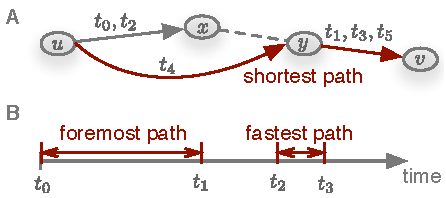
\includegraphics{Shortest_foremost_fastest.pdf}
\caption{Topological shortest distance and temporal shortest durations for a path between nodes $u$ and $v$.
The shortest path (Panel A) counts the number of edges between the nodes.
Panel~B demonstrates that although the fastest path could take $t_3-t_2 < t_1-t_0$, the foremost path arrives already at $t_1<t_2$.
}
\label{fig:shortest_foremost_fastest}
\end{SCfigure}
%
Note that possible paths between nodes depend on time in general.
This has crucial implications on the shortest path distance known from static networks (see section  \ref{sec:network_terminology}).
As a matter of fact, there are three different shortest path types in temporal networks.
Just like in the static case, the \emph{shortest} path distance between two nodes measures the topological distance between the nodes.
It counts the number of edges used do traverse the shortest path.
In addition, the \emph{duration} of a path can be measured in temporal networks.
This duration can be measured in two different time frames \citep{Casteights_review}:
First, the \emph{fastest} path between two nodes is the path of shortest duration, no matter when the path starts in time.
Second, the \emph{foremost} path between two nodes is the path that arrives earliest in a global time frame.

Figure~\ref{fig:shortest_foremost_fastest} demonstrates the difference between the foremost, fastest and shortest path concepts, respectively.
Edge labels are edge occurrence times, which are ordered so that $t_1<t_2<t_3<t_4<t_5$.
The dashed edge $(x,y)$ indicates that these nodes are not connected directly, but by other nodes of the network.
Panel A shows that the shortest topological path between nodes $u$ and $v$ is $(u,x,v)$ and the distance is $3$.
It can be seen from panel B that the first (foremost) path start at node $u$ at time $t_0$ and arrives at node $v$ at time $t_1$.
Although the fastest path takes less time to traverse ($t_3-t_2<t_1-t_0$), it arrives later ($t_3>t_1$) than the foremost path.
Note that shortest path and temporal shortest path do not coincide in this example, since the shortest path connection can be at times $t_4$ and $t_5$ which are greater than $t_1$ and $t_3$.

Throughout the rest of this work, we use a global time scale, which is defined by the first time in the dataset under consideration.
Consequently, we measure shortest path durations in terms of \emph{foremost} path durations, if not explicitly stated.

\subsection{Conceptual problems in temporal networks}\label{sec:conceptual_problems}
Before we focus on different methods to analyze temporal networks, we have to point out that many static network measures, such as centrality or components, are in general time-dependent and can not be summarized to static measures.
As an exception, \citeauthor{Grindrod:2011fg} defined a time-independent centrality measure for temporal networks \citep{Grindrod:2011fg}. 
In addition, time-scales of node dynamics and network dynamics can be of the same order and cause significant interactions between the dynamics.
We consider the relation between node dynamics and edge dynamics in Section~\ref{sec:Plos}.

The most essential difference between static and temporal networks lies in the importance of causality of paths in temporal networks.
Although it is possible to analyze paths in temporal networks systematically (see Section~\ref{sec:PRL}) we have to stress that generalizing the concept of connected components is far more complex in temporal networks as it is in the static case.
\citeauthor{Nicosia:2012hz} point out that finding connected components in temporal networks is NP-complete in general \citep{Nicosia:2012hz}.
In addition to that, the authors demonstrate that components in temporal networks can be \emph{degenerated}, i.e. there are multiple possible partitions of connected components and nodes can belong two multiple components at the same time.

We take up this point at the end of Section~\ref{sec:PRL}.
In order to get an impression about the path structure in temporal networks, we start with a pure data-analysis of a temporal network dataset. 

\section{Data driven network analysis}\label{sec:Plos}
In this section we analyze the livestock trade data set as introduced in Section~\ref{sec:network_analysis}, but we explicitly take into account temporal information%
\footnote{%
In order to be congruent with the datasets used in the publications, we use the pig trade dataset of \citep{Konschake:2013js} in this chapter.
This dataset differs slightly from the static network dataset used in Section~\ref{sec:network_analysis}.
It covers the period from 01 January 2008 to 31 December 2009.
The results do not change qualitatively and hereby the results of \citep{Konschake:2013js} and \citep{Lentz:2013PRL} are comparable.}. %
%
Each edge in the system is only present at certain days, i.e. the network can show bursty behavior and long waiting times between edge occurrences can be present in the system.

As in the case of static networks, the concept of centrality plays an important role for risk assessment and the implementation of vaccination and surveillance strategies also in time-varying topologies.
The maximum spreading potential of each node is given by its range as discussed for static networks in Section~\ref{sec:network_analysis}.
In this section we analyze the ranges of the network nodes according to their constance over time.
The results shown in this section are published in \citep{Konschake:2013js}.

\subsection{Representative sample}\label{sec:representative_sample}
Before we analyze the ranges of the nodes in the network, we estimate the time span needed to cover the temporal properties of the system.
Figure~\ref{fig:Plos_S1} A shows the activity of the nodes and edges in the network over the observation period.
The red line shows the number of active nodes on a daily resolution.
We observe that 25~\% of all nodes and 10~\% edges are active every day on average.
The plot shows decreased activity during the summer month and on public holidays such as easter and christmas.
In addition, there is a slight trend to a decrease of the number of nodes, which reflects a centralizing process in the system.
%
\begin{figure}[htbp]
\begin{center}
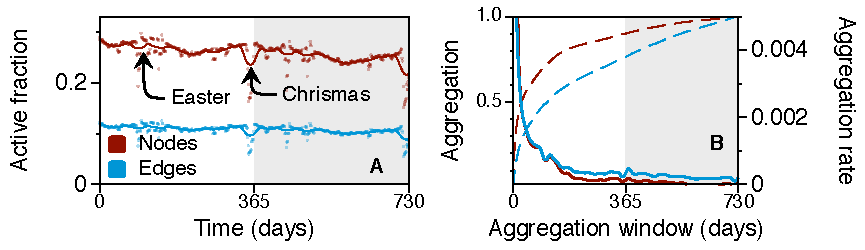
\includegraphics{Plos_S2AB.pdf}
\caption{\textbf{Panel A:} Daily activity of the livestock trade network over two years.
Original data is shown as points and solid lines are local regressions of the original data.\\
\textbf{Panel B:} Time aggregation of the network for different aggregation windows.
Dashed lines show the fractions of nodes/edges in the aggregated network.
Solid lines are local regressions of the aggregation rates.
}
\label{fig:Plos_S1}
\end{center}
\end{figure}

Figure~\ref{fig:Plos_S1} B gives a picture about the convergence of the network during the aggregation process, i.e. summing up the snapshots of the temporal system step by step to obtain the static network representation.
Dashed lines show the fractions of nodes and edges in the aggregated network, respectively.
The solid lines show the respective aggregation rates.
Since the latter are derivatives of the aggregation fractions, we show a local regression of the aggregation rate to reduce noise in the signal.

The figure demonstrates that the aggregation rates for both nodes and edges becomes negligible after 1 year.
Therefore, we can assess a period of 1 year sufficient to provide stationarity of the system, i.e. the time span, after which only few more edges are added to the network.

\subsection{Simulated disease outbreaks}
Node rankings are of major importance for epidemiology.
We try to answer the question, if a constant ranking of node makes sense in this particular temporal network.
As a generic measure for the spreading potential of a node, we consider its range.
In analogy to Section~\ref{sec:network_analysis}, we define the range of a node in a temporal network as the size of its temporal out-component.
It is important to note that the out-component of each node depends on the time $t_0$, when it is measured.
In addition to that, the range of a node can depend on the particular spreading process, e.g. an epidemic, a chemical reaction or rumor spread.
More specifically, a spreading process can have a finite memory $d$ that shortens the ability of a node to maintain in a certain state over time.
In our context, this memory corresponds to the \emph{infectious period} $d$ of a disease, i.e. the time period, after the infection dies out if it is not carried over to another agent.
Computing the range combined with a finite infectious period mimics an SIR-type process, where the infectious period is related to the reciprocal recovery rate as discussed in Section~\ref{sec:sir_model}.
For clarity reasons we do not solve differential equations for epidemics in this section and reduce the infection dynamics to assigning a discrete infection state -- susceptible, infected or recovered -- to each node in the network.
An infected node remains infected over the infectious period $d$.
Thus, the infection state of the whole network is given by the number of susceptible $S(t)$, infected $I(t)$ and recovered $R(t)$ nodes, respectively.

We define the \emph{temporal range} of a node $v$ by explicitly taking into account the time of (primary) infection and infectious period, i.e. $r(v,d,t_0)$.
Since there are no mixing states of nodes as in meta populations and we assume an infection probability $p=1$ for every contact edge, the range of a node is identical to the outbreak size $R(t=\infty )$. 

In summary, range and infectious period are intrinsically entangled on temporal networks
\begin{equation}\label{eq:range_and_inf_period}
\text{static network: } \; r(v) \;\;\; \rightarrow   \;\;\; \text{temporal network: } \; r(v,d) .
\end{equation}
For the rest of this work, we therefore use the notion \emph{range} and \emph{outbreak size} synonymously.
Although the temporal range should approach the static range for infinite memory, i.e. $r(v,d=\infty ) \rightarrow r(v)$, the static range of a node is in general not reached even in this case.
This is caused by causality of paths in temporal networks as explained in Figure~\ref{fig:temporal_network_principle}.

\subsubsection{Single outbreaks}
We address the outbreak pattern caused by single outbreaks in this section, while we discuss the properties of the set of all possible outbreak scenarios in the next section.
In order to analyze node ranges in the pig trade network, we use a modified breadth-first-search algorithm (see Appendix~\ref{sec:implementation} for a brief summary of search algorithms for static networks).
Given a fixed infectious period, we mark a particular node $v$ to be infected at time $t_0$.
For every time step $t$ in the interval $[t_0,t_0+d]$, we identify the neighborhood $\mathcal{N}(v,t)$ and mark all susceptible nodes in $\mathcal{N}(v,t)$ as infected.
Infected nodes are marked as removed after the infectious period $k$ and do not contribute to further infections.
This procedure is repeated for all infected nodes as long as there are still infected nodes in the system.

\begin{SCfigure}
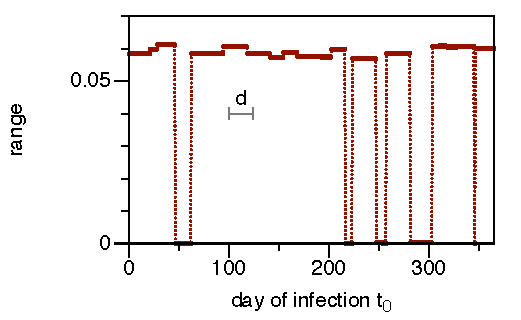
\includegraphics{exemplary_range.pdf}
\caption{Temporal variation in the range $r(v,d,t_0)$ of an exemplary node $v$ in the network over one year.
Although the range remains rather constant for most infection times, it vanishes for certain periods.
The grey interval corresponds to the fixed infectious period $d=24$~days.
}
\label{fig:range_exemplary}
\end{SCfigure}
%
Figure~\ref{fig:range_exemplary} shows the range of an exemplary node in the network for different infection times $t_0$.
The infectious period is $d=24$ days.
For most infection times the example node can infect about $6~\%$ of the network.
The range distribution over time shows a similar bimodal pattern similar to the distribution over nodes for the static network in Figure~\ref{fig:node_range}.
This provides evidence that there is an infection path from the exemplary node to a connected component in the network.
It is important to stress that the concept of connected components does not translate to temporal networks in a straightforward manner (see Section~\ref{sec:conceptual_problems}).
Besides the bimodality itself, it remarkable that the majority of adjacent primary infection times cause outbreaks of similar size.

This feature is can be explained, if we underline the temporal sparsity of edges, i.e. nodes are likely to have only few contacts within one infectious period.
If the primarily infected node $v$ has no trade contact within the infectious period, the disease dies out.
Even if the disease is transferred to a successor node $w$ at a time $t_1$ within the interval $[t_0,t_0+d]$, the disease dies out, if there is not further trade contact within the period $[t_1+d]$ and so forth.
The regions of small/vanishing range in Figure~\ref{fig:range_exemplary} correspond to these scenarios.
On the other hand, if all successors of node $v$ have one or more trading contact within their respective infectious periods, the disease can be transferred to a larger number of nodes.
The majority of small variations in $t_0$ implies stable ranges in the order of $d$ (the infectious period is shown by the grey line in Figure~\ref{fig:range_exemplary}).
If the degree of $v$ or a successor node in the infection chain is even larger than 1, even more secondary outbreaks are triggered and manifest themselves in smaller range fluctuations as for the long range values in Figure~\ref{fig:range_exemplary}.

We have seen in this section that a temporal degree of freedom adds a significant amount of complexity even to the outbreak pattern of a single node.
Now we focus on the set of \emph{all} outbreak scenarios, i.e. the set of all initial conditions and variations in the infectious period as a parameter.
%
\subsubsection{Set of outbreak scenarios}
We apply the method discussed in the previous section to all nodes in the network.
As primary infection times, we consider all times within the first year in the dataset.
This ensures that even if a particular outbreak penetrates the second year, it will have died out within the observation period.
We restrict ourselves to infectious periods $d<56$~days, since this interval covers the infectious periods of the major livestock diseases \citep{Horst:1998wu,Konschake:2013js}.
Considering all nodes in the network as potential starting points for infections and all days in the first year of the dataset as possible starting times yields $10^9$ different initial conditions.
We denote the \emph{set of all outbreak scenarios} by $\mathcal{S}$.
More formally, let $\mathcal{G}=(V,\mathcal{E},T)$ be the temporal network of our dataset.
Then the set of all outbreaks is given by all possible initial conditions and parameters and the corresponding outbreak size, where the latter is identical to the range for our model:
\begin{equation}\label{eq:outbreak_set}
\mathcal{S}=\left\{ (v,t_0,d,r(v,d,t_0)): v \in V,t_0 \in T/2, d \leq 56  \right\}.
\end{equation}
%
In what follows, we will average over this set in different ways to immediately obtain information about the impact of infectious period, primary infection time or the starting node on disease spread.
Table~\ref{tab:outbreak_set} shows a table representation of the set \eqref{eq:outbreak_set}.
%
\begin{table}[htb]
\sffamily
\begin{center}%\centering
\caption{Tabular data structure of the set of outbreak scenarios as defined by \eqref{eq:outbreak_set}.
We analyze 103,490 starting nodes for 365 times of primary infections and 56 different infectious periods yielding $10^9$ rows.
}
\begin{tabular*}{\hsize}{@{\extracolsep{\fill}}ccc|c}
\hline
~& initial conditions \& parameter  & ~ & result\\
\hline
Starting node & time of primary infection &infectious period & outbreak size \\
ID & $t_0$  &$d$ &$r(v,d,t_0)$  \\
\hline
1 & 1 & 1 & 58  \\
1 & 2 & 1 & 276  \\
\multicolumn{4}{c}{\vdots}\\%\vdots &\vdots &\vdots & \vdots \\
103,490 & 365 &56 & 72  \\
\hline
\end{tabular*}
\label{tab:outbreak_set}
\end{center}
\end{table}

Considering static networks, every node can cause an epidemic, if it is connected to other nodes in the network.
We have seen in the previous section that in temporal networks the time of primary infection has to be in an appropriate interval.
In addition, the range also depends on the infectious period, since a disease with high infectious period is more likely to spread over the network than a disease with low infectious period.
We define the \emph{outbreak probability} $p_s(d)$ as the fraction of elements in $\mathcal{S}$ that causes a secondary outbreak at all, that is
\begin{equation}\label{eq:outbreak_prob}
p_s(k)=\frac{\abs{\left\{ x \subset \mathcal{S}: r(v,d,t_0) \in x >0, d=\mathrm{const.} \right\}}}{\abs{\mathcal{S}}} .
\end{equation}
Note that we compute the outbreak probability for each infectious period separately.

Figure~\ref{fig:plosfig1} A shows the outbreak probability for different infectious periods.
For comparison, the outbreak probability in the static network is shown by the dashed line.
This is just the fraction of nodes with finite out degree and apparently the outbreak probability has no dependence on the infectious period in the static case.
The outbreak probability saturates for sufficiently large infectious periods, but it is still only half as much as in the static case even for $d=56$.
%
\begin{figure}[htb]
\begin{center}
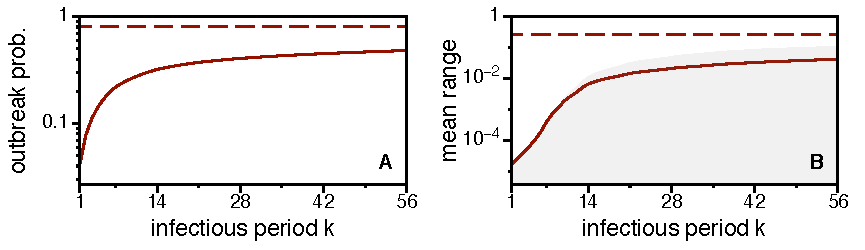
\includegraphics{Plos_fig1}
\caption{Outbreak probability (A) and mean range (B) for different infectious periods $d$ as solid lines.
Dashed lines correspond outbreak probability and mean outbreak size of the static network, respectively.
The grey shaded area in panel B shows the 50~\% confidence interval.}
\label{fig:plosfig1}
\end{center}
\end{figure}

In addition to the probability of an outbreak, we compute the expected size of the outbreaks.
The \emph{mean outbreak size} is an average over all starting nodes and all starting times in $\mathcal{S}$, i.e. $\mean{r(v,d,t_0)}_{v,t_0}$.
Figure~\ref{fig:plosfig1} B shows the mean outbreak size and the 50~\% confidence interval (solid line and grey shaded area) and the mean outbreak size in the static network (dashed line).
As for the outbreak probability, we observe significant outbreak sizes only for $d>14$~days and the outbreak size is 6 times smaller than in the static case even for $d=56$~days.
In summary, the infectious period must be larger than 14~days to cause a severe outbreak and the static network approximation overestimates the size of outbreaks significantly.

\subsection{Node rankings}
This section is devoted to the analysis of the node ranking according to their respective ranges.
Rankings are very important for the implementation of vaccination and surveillance strategies, where the exact value of a certain measure for each node is not important.
%In fact, the \emph{ordering}
For every infectious period $d$, we average over all times of primary infection in \eqref{eq:outbreak_set}.
Thus, $b(v,d)=\mean{r(v,d,t_0)}_{t_0}$ is a function of the node and infectious period.
Ordering $b(v,d)$ for every $d$ in descending order gives a ranking $R(d)$ of the nodes according to their outbreak sizes, where $R(d)$ is an ordered set of nodes for every infectious period.
The question is, whether these rankings remain stable, if the infectious period is changed.

Figure~\ref{fig:ranking} shows the ranking trajectories over different infectious periods of the top 100 nodes in the network. 
We define the top 100 nodes as the nodes with the largest outbreak size in $\mathcal{S}$ averaged over both $t_0$ and $d$, i.e. $\mean{r(v,d,t_0)}_{d,t_0}$.
An arbitrarily chosen node is shown in red for illustration purposes.
It should be noted that the rank of each node in the top 100 set can take any value in the figure, since the top 100 nodes are determined by averaging out the infectious period.

As the figure suggests, the ranking of nodes is unstable for small infectious periods ($d<21$~days).
This region is dominated by temporal fluctuations of the infection paths in the network.
Interestingly, the ranking approaches a stable region for $d>21$~days.
For $d>28$~days most nodes in the top 100 sample do not undergo significant rank changes any more.
This means that a ranking of nodes is reasonable for sufficiently large infectious periods.
%
\begin{SCfigure}
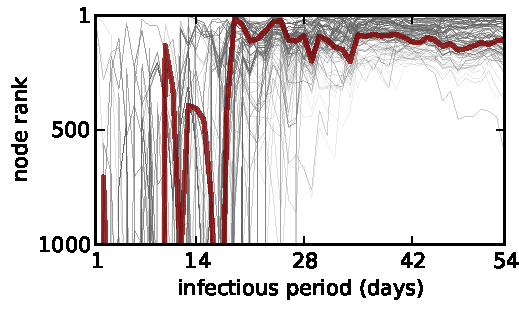
\includegraphics{vir_ranking.pdf}
\caption{Node ranking of the top 100 nodes over different infectious periods.
Rankings are computed by averaging \eqref{eq:outbreak_set} over the time of primary infection.
Top 100 nodes are the nodes with the largest outbreak sizes averaged over $d$ and $t_0$.
The rankings of an arbitrary node are shown in red for illustration purposes.}
\label{fig:ranking}
\end{SCfigure}

\subsection{Inaccurate infectious periods and the robustness of node rankings}
Finding exact values of the infectious periods of a certain disease is often unachievable in real world scenarios.
Therefore, we look into the impact of variations in the infectious period on the ranking of nodes.
We consider pairs of rankings as defined in the previous section with different infectious periods, i.e. $R(d_1)$ and $R(d_2)$.

In order to compare two rankings, we could use measures of rank correlation, such as Spearman or Kendall rank correlation coefficients.
These turn out, however, to be very sensitive to even small differences between two rankings.
Figure~\ref{fig:ranking} suggests that even in the stable region where $d>28$~days node ranks remain similar, but not equal.
Computing Spearman or Kendall rank correlation coefficients for different infectious periods $(k_1,k_2)$ in our dataset would give vanishing values for almost all pairs $(d_1,d_2)$.
For that reason, we relax the requirements for similarity between to rankings.
Thus, we consider the \emph{intersection} between the sets of the respective upper samples of each ranking.
In other words, we examine whether the same nodes appear in the upper ranks of both the $R_{d_1}$ and the $R_{d_2}$ rankings.

We denote the subset of the upper $\tau $ ranks of $R(d)$ by $R_\tau (d)$.
As a similarity measure, we define the \emph{rank intersection} between two rankings $R_\tau (d_1)$ and $R_\tau (d_2)$ as
\begin{equation}\label{eq:rank_intersection}
s_\tau (d_1,d_2)=\frac{R_\tau (d_1) \cap R_\tau (d_2)}{\abs{R_\tau (d_1)}},
\end{equation}
that is the intersection between the sets of nodes normalized by the size of the top $n$ sample.
We get $s_\tau (d_1,d_2) =1$, if the upper $\tau $ nodes in the rankings $R(d_1)$ and $R(d_2)$ are identical.
On the other hand, $s_\tau (d_1,d_2) =0$ implies that ranks for $d_2$ and $d_2$ are completely different.

Using Equation~\eqref{eq:rank_intersection} yields a similarity matrix with $1540$ different combinations of infectious periods for our outbreak scenarios \eqref{eq:outbreak_set}.
Since particular combinations of infectious periods are not relevant, we analyze the \emph{uncertainty} of the infectious period
\begin{equation}\label{eq:uncertainty_k}
\Delta d= \abs{d_1-d_2} .
\end{equation}
Now we average the entries of the similarity matrix over uncertainties and get the rank intersection
\begin{equation}\label{eq:robustness_k}
\tilde{s}_\tau (\Delta d)=\mean{s_\tau (d_1,d_2)}_{\abs{d_1-d_2}\leq \Delta d} .
\end{equation}
This rank intersection measures the robustness of a certain ranking against changes in the infectious period.
Therefore, we call this measure the \emph{rank robustness} a given uncertainty in the infectious period.
%
\begin{SCfigure}
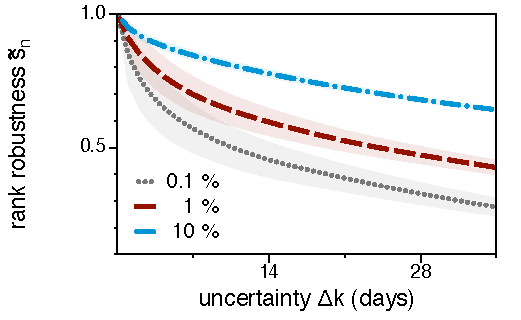
\includegraphics{Plos_fig4a.pdf}
\caption{Rank robustness vs. uncertainty in the infectious period for the upper $0.1$~\% (grey), $1$~\% (red) and $10$~\% (blue) of nodes in the network.
Shaded areas correspond to the $50$~\% confidence intervals.}
\label{fig:plos_fig4a}
\end{SCfigure}

For convenience, we express \eqref{eq:robustness_k} in terms of the upper \emph{fraction} of nodes instead of the upper nodes themselves.
That is, we replace the top $\tau $ nodes by the top fraction of nodes $n$:
\begin{equation}\label{eq:rank_robustness}
\tilde{s}_n (\Delta d)=\mean{s_n (d_1,d_2)}_{\abs{d_1-d_2}\leq \Delta d} .
\end{equation}
The same is implicitly done for rank intersection $s_n(d_1,d_2)$ \eqref{eq:robustness_k} and the node ranking $R_n(d)$.

We show the rank robustness for the fraction of the $0.1$~\%, $1$~\% and $10$~\% upper nodes in Figure~\ref{fig:plos_fig4a}.
These fractions correspond to approximately 100, 1000 and 10,000 nodes, respectively.
The $50$~\% confidence intervals of each curve are shown as shaded areas.
As expected, larger uncertainty in the infectious period generally leads to a decrease of rank robustness.
The decrease is small for the largest sample (blue), since the number of nodes in this sample is relatively large.
This guarantees that the same nodes are likely to be in all rankings $R_{10\%}(d)$ for all $d$.  
Consequently, the variation in rank robustness is relatively small (blue shaded area).
Considering the 0.1~\% sample (grey), it is remarkable that even for an uncertainty of 14~days, the robustness is still 50~\%.
As a smaller sample is more prone to fluctuations, variations of rank robustness are relatively large (grey shaded area).
The red curve shows an intermediate behavior.

\subsection{Temporal vs. static representation}
Since the analysis of a temporal network using a data driven approach is computationally expensive, we compare the node rankings $R_n(k)$ to centrality measures for the static network representation as defined in Section~\ref{sec:micro_measures}.
We denote the upper $\tau $ nodes according to a static centrality measure as $C_\tau $.
Note that $C_\tau $ does not depend on the infectious period, since the latter plays no role in static networks.
In this work, we consider betweenness, closeness, degree centrality and range as centrality measures.
Following Equation~\eqref{eq:rank_intersection}, we define the \emph{centrality intersection} between the outbreak size ranking $R_\tau (d)$ and $C_\tau $ as
\begin{equation}\label{eq:centrality_intersection}
I_\tau (k)=\frac{R_\tau (d) \cap C_\tau}{\abs{C_\tau}},
\end{equation}
where $C_\tau $ is a substitute for the upper $\tau $ nodes of one particular centrality measure listed above.
%
\begin{figure}[htb]
\begin{center}
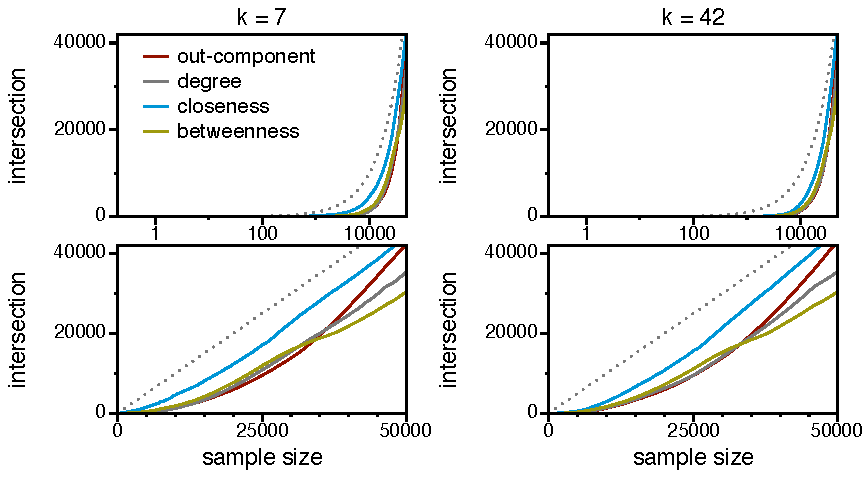
\includegraphics{Plos_fig5.pdf}
\caption{Intersection between outbreak size and different static centrality measures.
\textbf{Left~panel:}~infectious period $d=7$~days.
\textbf{Right~panel:}~infectious period $d=42$~days.
Top panels show $x$-log versions of the bottom panels. 
Dotted lines show data accordance $y=x$ for comparison.
The top panels demonstrate that finite intersections appear only for sample sizes of more than 1000 nodes.}
\label{fig:plos_fig5}
\end{center}
\end{figure}

In Figure~\ref{fig:plos_fig5}, we plot the centrality intersection \eqref{eq:centrality_intersection} for different static centrality measures and two exemplary infectious periods.
Upper panels are identical to the lower panels, but use logarithmic $x$-axes. 
The upper figures show that non vanishing intersections are taken for samples of at least 1000 nodes.
Consequently, the upper part of the ranked nodes does not coincide with high ranked nodes in any static centrality measure.
Intersections between outbreak size and static centrality measures become significant only for sample sizes of more than 10,000 nodes, i.e. about 10~\% of the network!
Although this fraction is rather large, the coincidence of centrality and outbreak size is still relatively small, as can be seen when comparing the centrality curves to the dotted line on the lower panel.
The different centrality measures show similar intersections with the outbreak size.
An exception is closeness centrality, which performs significantly better than the other measures.
An explanation for this special role is that nodes with high closeness are likely to infect other nodes within only few steps as it follows from the definition of closeness.
This way long static paths are avoided, i.e. the chance that one of these static paths is disrupted by causality is relatively low.
It should be noted that all features discussed above are almost identical for both infectious periods.

\paragraph{Summary of the data-driven analysis\color{Cayenne}{.}}
We simulated an SIR-type disease on the livestock trade dataset and explicitly took into account the temporal dynamics of edges.
This yields a set of outbreak scenarios, which can be thought of as a scalar-field $r(v,d,t_0)$, where each triple $(v,d,t_0)$ is assigned an outbreak size $r$, if $r>0$.
A schematic sketch of this scalar-field is given in Figure~\ref{fig:Plos_parameter-space}.
%
\begin{SCfigure}
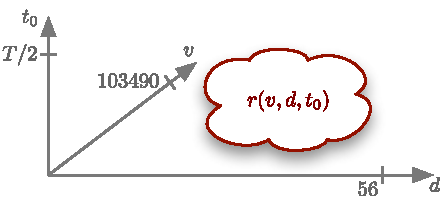
\includegraphics{Plos_parameter-space.pdf}
\caption{Scalar field representing the set of outbreak scenarios as defined in \eqref{eq:outbreak_set}.
Each combination of starting node $v$, starting time $t_0$ and infectious period $d$ yields an outbreak size $r(v,d,t_0)$.
The domain is bounded as defined in \eqref{eq:outbreak_set}.}
\label{fig:Plos_parameter-space}
\end{SCfigure}
%
Using the state space of Figure~\ref{fig:Plos_parameter-space}, we can summarize the different aggregation techniques used in this section as follows:
\begin{description}
\item [Exemplary outbreak:] All outbreak sizes for a cut through $r$ for constant $d$ and $v$ (see Figure~\ref{fig:range_exemplary}).
\item [Outbreak probability:] State density of $r$ for every $d$-slice of the state space (see Figure~\ref{fig:plosfig1}~A).
\item [Mean outbreak size:] The mean value of the field in every $d$-slice (see Figure~\ref{fig:plosfig1}~B).
\item [Node ranking:] First, average over the $t_0$-axis. Afterwards ordering of nodes by largest outbreak size for every $d$-slice. See Figure~\ref{fig:ranking}.
\item [Infectious period uncertainty:] Comparison between pairs of node rankings. See Figure~\ref{fig:plos_fig4a}.
\end{description}
%
The comparison to the static network representation (figure~\ref{fig:plos_fig5}) is obtained using intersections between pairs of node rankings in analogy to the estimation of uncertainty of the infectious period.

We conclude that although the temporal nature of the system results in strong fluctuations of the paths in the network, a ranking of nodes according to their range appears reasonable for sufficiently large infectious periods.
This ranking could not be reproduced using classical static centrality measures.
In addition to that, a static network view systematically overestimates disease outbreaks in the network.
Even for large infectious periods, we found the mean outbreak sizes to be six times smaller as for the static case.

\section{Graph centric temporal network analysis}\label{sec:PRL}
The previous section has shown that even the analysis of simple measures such as node ranges is a complex endeavor.
While the previous section implicitly used a node centric approach to the system, we now introduce a \emph{graph centric} approach to temporal networks.
It is important to emphasize that the capability of static network analysis originates from the fact that the adjacency matrix provides a graph centric (``big picture'') of the system.
Therefore, a graph centric view for temporal networks contributes a key element for a theoretical framework for temporal systems.

As we have seen in Section~\ref{sec:paths_in_temporal_networks}, the static approximation of a temporal network leads us to believe that all paths are transitive and therefore lacks a differentiation between causal and non causal paths.
We make use of adjacency matrix sequences as defined by Equation~\eqref{eq:AdMatrixSequence} and derive a method for the computation of causal paths.

This yields first the ranges of all nodes in the network and second information about the mutual \emph{accessibility} between nodes.
In analogy to the static range defined in Equation~\eqref{eq:range_def}, the range of a node $v$ in a temporal network $\mathcal{G}=(V,\mathcal{E},T)$ can formally be defined as
\begin{equation}\label{eq:temporal_range_def}
r(v)=\frac{\left| \mathcal{H}(v) \right| }{N}, \; \text{ where } \; \mathcal{H}(v)=\{u \in V: v\rightsquigarrow u \},
\end{equation}
where $\mathcal{H}(v)$ is the horizon of node $v$ and $N$ the number of nodes in the network.

The set of all horizons in a network defines its \emph{accessibility graph}.
For static networks, the concept of accessibility was defined at the end of Section~\ref{sec:macro_measures}.
We extend the static accessibility approach to the explicit step by step derivation of accessibility in Section~\ref{sec:unfolding_static}.
This novel procedure is called \emph{unfolding} of accessibility.
Finally, we generalize the unfolding accessibility approach to temporal networks in Section~\ref{sec:unfolding_temporal}.
The results presented in this section are in part published in \citep{Lentz:2013PRL}.

\subsection{Accessibility of static networks}\label{sec:unfolding_static}
We consider a static network $G=(V,E)$ with $N$ nodes and adjacency matrix $\mathbf{A}$.
The accessibility graph (or transitive closure) of $G$ is denoted by $G^*=(V,E^*)$, where $E^*$ contains an edge $(u,v)$, whenever $u\rightarrow v$.
The accessibility matrix -- i.e. the adjacency matrix of the accessibility graph -- can be computed using the cumulative matrix defined by
\begin{equation}\label{eq:cumulative_matrix2}
\mat{C}_n=\mat{A}+\mat{A}^2+\cdots + \mat{A}^n = \sum _{i=1} ^n \mat{A}^i .
\end{equation}
%This equation was already introduced in Section~\ref{sec:macro_measures}.
Every term $\mat{A}^i$ corresponds to a network where nodes are connected that have shortest path distance $i$ in G.
Figure~\ref{fig:power_graphs} illustrates this observation.
%
\begin{SCfigure}
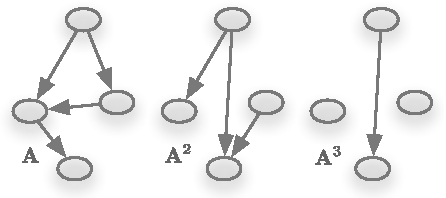
\includegraphics{Power-graphs.pdf}
\caption{Graph representations of different powers of an adjacency matrix.
The left panel shows the original graph $G$ with adjacency matrix $\mat{A}$.
Node pairs with distance 2 in $G$ are connected by an edge in the graph of $\mat{A}^2$ (middle).
The analogue for distance 3 is shown on the right panel.}
\label{fig:power_graphs}
\end{SCfigure}

In general, each power of an adjacency matrix contains the number of paths between node pairs as entries.
Since we are not interested in the actual \emph{number} of paths, we can treat the adjacency matrix as Boolean and use Boolean arithmetic and normal algebra.
Thus, the normalized cumulative matrix can be computed using
\begin{equation}\label{eq:static_boolean_acc}
\mathbf{P}_{n}=\bigvee _{i=1} ^{n} \mathbf{A}^i ,
\end{equation}
where the $i$-th power of the adjacency matrix is computed using the matrix product of two Boolean matrices $\mathbf{A}$ and $\mathbf{B}$ defined by 
\begin{align}\label{eq:boolean_product}
(\mat{A}\mat{B})_{ij}&=(a_{i1}\wedge b_{1j})\vee \dots \vee(a_{iN}\wedge b_{Nj}) \nonumber \\
&= \bigvee _{k=1}^N a_{ik} \wedge b_{kj} .
\end{align}
In Equations~\eqref{eq:static_boolean_acc} and \eqref{eq:boolean_product}, $\vee $ denotes a Boolean OR and $\wedge $ a Boolean AND, respectively.

The adjacency matrix of the accessibility graph is given by $\mathbf{P}_{n=N-1}$.
We call $\mathbf{P}_{N-1}$ the \emph{accessibility matrix} of $G$.
Note that the index $N-1$ corresponds to the maximum path length in the network.
The graph $G^*$ given by $\mathbf{P}_{N-1}$ is called fully exploited accessibility graph.
We focus on accessibility for values other than $N-1$ below.

\paragraph{Properties of accessibility graphs\color{Cayenne}{.}}
In a \emph{connected} network $G$, the graph $G^*$ contains links between all node pairs, since all nodes are connected by a path.
Thus, $G^*$ is fully connected and the matrix $\mathbf{P}_{N-1}$ has only nonzero entries.
It follows from the transitivity of paths that also all entries $(\mathbf{P})_{ii}$ are unity, since there is always a path from node $i$ to some other node $j$ and vice versa.
Consequently, $\mathbf{P}_{N-1}$ has $N^2$ nonzero entries in this case.
If the network $G$ is \emph{not connected}, the accessibility matrix can be transformed into a block diagonal form, where each block has only nonzero entries.
The total number of nonzero elements in this case is smaller than $N^2$.

%
\begin{figure}[htb]
\begin{center}
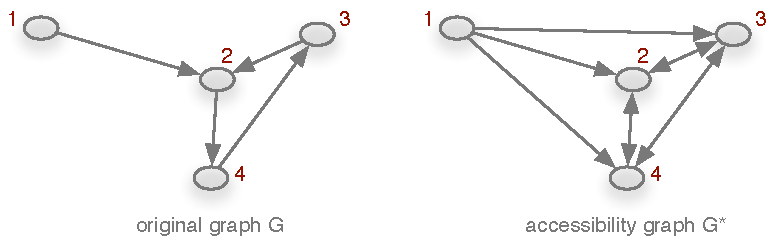
\includegraphics{Accessibility_principle_static.pdf}
\caption{A static network $G$ and its accessibility graph $G^*$.
The nodes 2, 3 and 4 are strongly connected in $G$ and form a clique in $G^*$.}
\label{fig:access_static}
\end{center}
\end{figure}
%
Figure~\ref{fig:access_static} shows the accessibility graph of a static network.
The corresponding accessibility matrix is
\begin{equation*}
\mathbf{P}_N=\left(%
\begin{array}{c|ccc}%
0 & 1 & 1 & 1 \\
\hline 0 & 1 & 1 & 1 \\
0 & 1 & 1 & 1 \\
0 & 1 & 1 & 1
\end{array}\right) .
\end{equation*}
The nodes of the connected components in the adjacency matrix $\mathbf{A}$ form blocks in $\mathbf{P}_N$ so that nodes 2, 3 and 4 form a fully connected subgraph (clique) in $G^*$.

If the network $G$ is \emph{undirected}, every $\mathbf{P}_n$ has a non vanishing main diagonal for $n\geq 2$, if there are no isolated nodes.
This corresponds to the fact that there is always a path of length 2 from a node back to itself.
For the directed case, the main diagonal of $\mathbf{P}_{N-1}$ can contain 0 or 1 entries.

\paragraph{Shortest paths and unfolding accessibility\color{Cayenne}{.}}
Now we focus on the properties of the accessibility graph for the steps $\mathbf{P}_{n\leq N}$.
We explicitly take into account different values of $n$, i.e. we \emph{unfold} the accessibility graph.
Each $\mat{P}_n$ is the adjacency matrix of a preliminary accessibility graph, which we denote by $G_n ^*$.
The graph $G_1 ^*$ (with adjacency matrix $\mat{P}_1$) gives a graph containing paths of length 1, i.e. the adjacency matrix itself.
Analogues to Figure~\ref{fig:power_graphs}, the graph $G_2 ^*$ contains paths of length 1 \emph{and} paths of length 2.
In principle, the procedure $\mat{P}_n \rightarrow \mat{P}_{n+1}$ corresponds to traversing the graph by paths of one more edge.
This is equivalent to a breadth-first-search (BFS) algorithm in the network, which is a standard procedure in computational network analysis.
The BFS technique is explained in Appendix~\ref{sec:implementation}.
A similar method was used in early algorithms for computing shortest path lengths in networks \citep{Floyd:1962vo,Warshall:1962wr}.
At the moment, when the BFS-algorithm approaches the diameter $D$ of the network, the matrix $\mat{P}_n$ saturates and does not change for higher values of $n$.
Moreover, the accessibility matrix of a network is reached for $n=D$, so that
\begin{equation}\label{eq:diameter_sat}
\mat{P}_{D}\equiv \mat{P}_{D+1}\equiv \mat{P}_{N-1}.
\end{equation}
Hence, it is sufficient to compute only the first $D$ term in Equation~\eqref{eq:static_boolean_acc}.

The relation between the computation of accessibility and the BFS-algorithm suggests that this procedure contains information about the shortest path length distribution.
In order to reveal this correlation, we define the \emph{density} of a matrix $\mat{M}$ as the number of its nonzero elements, i.e.
\begin{equation}\label{eq:matrix_density}
\rho (\mat{M}) =\frac{\mathrm{nnz}(\mat{M})}{N^2}.
\end{equation}
In Equation~\eqref{eq:matrix_density} the number of nonzero elements is $\mathrm{nnz}(\mat{M})$ and $N$ is the dimension of $\mathbf{M}$.
As a special case, we define the \emph{path density} of a  network as the density of its accessibility matrix
\begin{equation}\label{eq:path_density}
\rho (\mat{P}_n) =\frac{\mathrm{nnz}(\mat{P}_n)}{N^2}.
\end{equation}
Note that the normalization in \eqref{eq:matrix_density} and \eqref{eq:path_density} is not $N(N-1)$, since we explicitly take into account self loops in the accessibility graph.
These self loops guarantee that the maximum path density is unity in connected graphs.

Now we address the relation between path density and shortest path distribution.
In the case of the adjacency matrix, Equation~\eqref{eq:matrix_density} gives the edge density of the network, which is equivalent to the probability that two randomly chosen nodes are connected by an edge.
It follows that the probability that two nodes are connected by a path of length $n$ is given by $\rho (\mat{A}^n)$.

Since the path density $\rho (\mat{P}_n)$ follows from a cumulative procedure, it corresponds to the probability that two randomly chosen nodes are connected by a path of length $l\leq n$.
Consequently, the path density is the cumulative distribution of shortest path lengths
\begin{equation}\label{eq:cumulative_distribution}
\rho (\mat{P}_n)=F(l\leq n)\equiv F_n .
\end{equation}
The shortest path length distribution follows from Equation~\eqref{eq:cumulative_distribution} by differentiation.
Since the step length is 1 by definition, the probability for a shortest path length $n$ is given by $f_n=(F_n-F_{n-1})$ and $F_0=0$.

It should be noted that the probabilities considered here are normalized to unity only for connected networks, because for connected networks $\rho (\mat{P}_{N-1})\equiv \mat{P}_D=1$.
In the case of disconnected networks, the saturation value is in general smaller than 1.
Therefore,  we treat the distribution \eqref{eq:cumulative_distribution} as an ``improper'' probability distribution, which is in general not normalized to unity.
In addition, we define the \emph{median} of $F_n$ as the value $n$ where $F_n=1/2 \; F_D$.

We make use of the relations discussed above in order to obtain information about the shortest path distribution.
We call this procedure \emph{Unfolding Accessibility}, because we explicitly analyze the step-by-step derivation of the accessibility matrix.
Although the concept of unfolding accessibility seems to make things unnecessarily complicated, it can be generalized to temporal networks.

But before we generalize the approach explained above to temporal networks, we illustrate the concept exemplarily for a static \ER network.
We compute the shortest path length distribution of a directed \ER network of 1000 nodes and 2000 edges.
Figure~\ref{fig:er_histo} shows the path density $\rho (\mat{P}_n)$ and the shortest path distribution.
The shortest path length distribution is identical to that of Figure~\ref{fig:ER_shortest_path_histogram} (section \ref{sec:er_model}).
%
\begin{figure}[htbp]
\begin{center}
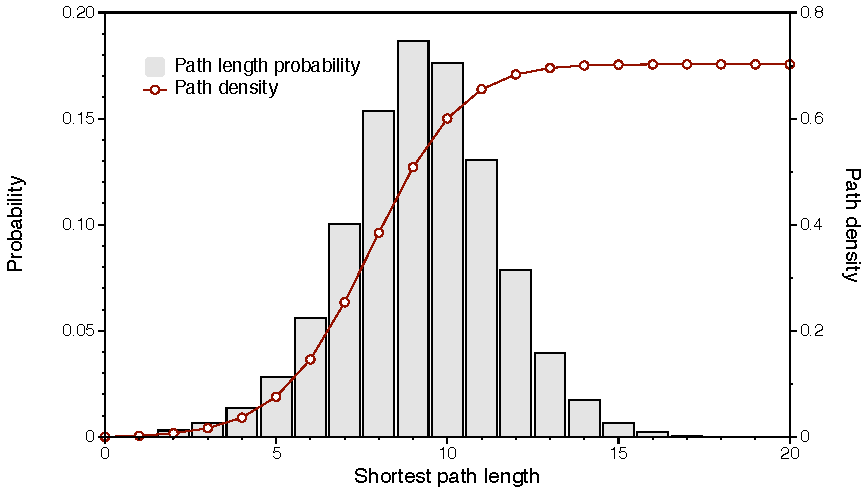
\includegraphics{ER_shortest_path_histo_double.pdf}
\caption{Path density (red line) and shortest path length distribution (grey histogram) for a directed \ER network with 1000 nodes and 2000 edges.
Mean value $8.18$, median $n=8$, diameter $D=18$, maximum path density $\rho (\mat{P}_D\approx 0.7)$.
The histogram is identical to that in Figure~\ref{sec:er_model}, where a standard BFS algorithm was used.
}
\label{fig:er_histo}
\end{center}
\end{figure}
%

\subsection{Unfolding Accessibility of temporal networks}\label{sec:unfolding_temporal}
We generalize the definition of the static accessibility matrix \eqref{eq:static_boolean_acc} to the case of temporal networks.
The basic problem is how to generalize different powers of an adjacency matrix to the case, where the adjacency matrix is not constant.
Let us consider a temporal network $\mathcal{G}=(V,\mathcal{E},T)$ with adjacency matrix sequence as defined in \eqref{eq:AdMatrixSequence}
\begin{equation}\label{eq:AdMatrixSequence2}
\mathcal{A}=\mat{A}_1,\dots ,\mat{A}_T .
\end{equation}
Treating each element $\mat{A}_t$ in $\mathcal{A}$ as Boolean, the aggregated network is given by the Boolean sum of the matrices
\begin{equation}\label{eq:aggregation}
\mat{A}=\bigvee _{t=1} ^{T} \mathbf{A}_t .
\end{equation}
Before we derive an expression for the accessibility graph $\mathcal{G}^*=(V,\mathcal{E}^*,T)$, we have to discuss the meaning of matrix multiplication in temporal networks.
In particular, we have to discuss the role of causality in paths generated by matrix products.
As shown in Figure~\ref{fig:power_graphs}, a product of adjacency matrices gives information about paths of a certain length in static networks.
The multiplication of two different matrices $\mat{A}_1$ and $\mat{A}_2$ yields nonzero entries, i.e. paths of length 2, wherever nodes of the graph of $\mat{A}_1$ receive links at time 1 and cast forth links at time 2.
An example is illustrated in Figure~\ref{fig:matrix_product}.
%
\begin{figure}[htb]
\begin{center}
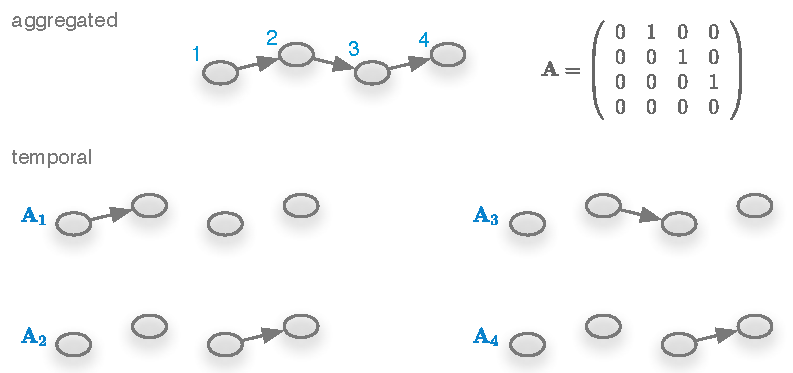
\includegraphics{Matrix_product.pdf}
\caption{Snapshots of a temporal network.
Each snapshot is given by an adjacency matrix $\mat{A}_t$.
The aggregated network and adjacency matrix are shown in the top panel.}
\label{fig:matrix_product}
\end{center}
\end{figure}
%
If we exemplarily multiply the two snapshots $\mat{A}_2$ and $\mat{A}_3$, we get
\begin{equation}\label{eq:matrix_multi_example}
\mat{A}_3 \mat{A}_4=\left( \begin{array}{cccc}%
0 & 0 & 0 & 0 \\
 0 & 0 & 1 & 0 \\
0 & 0 & 0 & 0 \\
0 & 0 & 0 & 0 \end{array} \right)%
\left( \begin{array}{cccc}%
0 & 0 & 0 & 0 \\
 0 & 0 & 0 & 0 \\
0 & 0 & 0 & 1 \\
0 & 0 & 0 & 0 \end{array} \right)%
=%
\left( \begin{array}{cccc}%
0 & 0 & 0 & 0 \\
 0 & 0 & 0 & 1 \\
0 & 0 & 0 & 0 \\
0 & 0 & 0 & 0 \end{array} \right).%
\end{equation}
Thus, there is a two-step-path from node 2 to 4 via node 3.
It follows that multiplication of different matrices is a reasonable operation for the computation of paths also in temporal networks.
Therefore a a straight-forward temporal generalization of the accessibility matrix could be to replace the power of adjacency matrices by products of different snapshots.
Defining $\tilde{\mathcal{C}}_n$ as the temporal generalization of \eqref{eq:cumulative_matrix2} and $\tilde{\mathcal{P}}_n$ as its Boolean version, this approach reads
\begin{equation*}%\label{eq:}
\tilde{\mathcal{C}}_n= \sum _{i=1} ^n \prod _{j=1} ^i \mathbf{A}_j = \mathbf{A}_1 + \mathbf{A}_1 \mathbf{A}_2 + \mathbf{A}_1 \mathbf{A}_2 \mathbf{A}_3 + \cdots
\end{equation*}
and
\begin{equation}\label{eq:wrong_access}
\tilde{\mathcal{P}}_n= \bigvee _{i=1} ^n \bigwedge _{j=1} ^i \mathbf{A}_j = \mathbf{A}_1 \vee \mathbf{A}_1 \mathbf{A}_2 \vee \mathbf{A}_1 \mathbf{A}_2 \mathbf{A}_3 \vee \cdots ,
\end{equation}
respectively.
Although this naive approach shows great similarities with the accessibility matrix of a static network, it turns out that it has a crucial drawback:
If we compute the product $\mat{A}_1 \mat{A}_2$ in Figure~\ref{fig:matrix_product}, we would get a zero matrix
\begin{equation}\label{eq:zero_matrix_product}
\mat{A}_1 \mat{A}_2 = \mat{0} .
\end{equation}
It follows from Equation~\eqref{eq:wrong_access} that $\tilde{\mathcal{P}}_n =\mat{A}_1$ for all $n=2$. 
As opposed to this, Figure~\ref{fig:matrix_product} suggests that the accessibility graph should contain other paths than $1\rightsquigarrow 2$ only, for example $1\rightsquigarrow 4$.
Apparently, the elements of the matrix products in \eqref{eq:wrong_access} become zero, if the requirement of receiving links at time $t$ and casting forth links at time $t+1$ is violated.
In a more general sense, the accessibility matrix given in Equation~\eqref{eq:wrong_access} gives meaningful results in the case that temporal correlations are only between successive snapshots of the system.
Systems with this property can be considered as Markovian temporal networks.

Many systems, however, show a \emph{bursty} behavior, i.e. significant waiting times between periods of node activity.
As an example, a typical trade pattern in the pig trade network used in sections \ref{sec:Plos} and \ref{sec:network_analysis} would be that animals remain at different holdings for certain periods of time for breeding or fattening. 
In these systems, consecutive matrices are not correlated and their products would vanish, i.e.
\begin{equation}\label{eq:limit_vanish_access}
\lim _{n\rightarrow \infty } \bigwedge _{t=1} ^n \mat{A}_t =\mat{0}.
\end{equation}
Equation \eqref{eq:limit_vanish_access} implies that all long time information would be lost.
This dilution of the path density occurs, if the temporal resolution of the dataset provides many snapshots over the typical timescale of the node waiting times.
As a consequence, these snapshots show relatively low edge densities.
\citeauthor{Bajardi:2011iv} reported a maximum path length of 8 days for a temporal cattle trade network, when edge sequences are at successive time steps \citep{Bajardi:2011iv}.

In order to overcome the drawbacks of Equation~\eqref{eq:wrong_access}, we explicitly take into account products of matrices over distant time steps.
In the example of livestock trade networks, a subset of nodes of the system could for instance fatten livestock animals for a timespan $\tau $.
Thus, these nodes receive links at time $t_1$ and cast forth links at time $t_2=t_1+\tau $.
More general, the time span $\tau $ could correspond to a production time in value chains or the period of stay at one place in human mobility networks.

On the whole, we have to include \emph{all} possible higher order products into the computation of the accessibility matrix.
It turns out that this is equivalent to adding a memory into the system, i.e. the ability of each node to keep edge information over time.
This can be done using self-loop so that we add an identity matrix $\mat{I}$ to each matrix in the sequence $\mathcal{A}$.
Then the unnormalized accessibility matrix of a temporal networks reads
%
\begin{align*}
\mathcal{C}_n=&\prod _{i=1} ^n (\mat{I} + \mat{A}_i ) \\
=& \mat{I}+\underbrace{ \mat{A}_1+\mat{A}_2+\mat{A}_3+\cdots + \mat{A}_n}_{\mat{A}} + \nonumber \\
&+ \underbrace{\mat{A}_1\mat{A}_2+\mat{A}_2\mat{A}_3+ \mat{A}_1\mat{A}_3+ \mat{A}_1\mat{A}_2\mat{A}_3 +\cdots }_{\mathcal{O}(\mat{A}_i ^2)}\nonumber .
\end{align*}
Since the actual number of paths are not important in this work, we define the the \emph{accessibility matrix of a temporal network} in Boolean notation
%
\begin{align}
\mathcal{P}_n=&\bigwedge _{i=1} ^n (\mat{I} \vee \mat{A}_i ) \label{eq:temporal_accessibility} \\
= & \mat{I}\vee \mat{A}_1\vee \mat{A}_2\vee \mat{A}_3\vee \cdots \vee \mat{A}_n \vee \nonumber \\
& \vee \mat{A}_1\mat{A}_2\vee \mat{A}_2\mat{A}_3\vee  \mat{A}_1\mat{A}_3\vee  \mat{A}_1\mat{A}_2\mat{A}_3 \vee \cdots . \nonumber
\end{align}
%
In Equation~\eqref{eq:temporal_accessibility}, the linear terms correspond to the aggregation of the network over $n$ time steps.
These are all paths of length 1, which are always causal.
The higher order products always respect the temporal correct order of snapshots, that is $i<j$ for all $\mat{A}_i\mat{A}_j$ and $\mat{A}_i \cdots \mat{A}_j $.
Analogue to Section~\ref{sec:unfolding_static}, we define the accessibility graph to path duration $n$ as $\mathcal{G}_n ^*$

It should be noted that in general the ``real'' accessibility graph of a temporal network is given by $\mathcal{G}_\infty ^*$, since the observation time is limited and might not capture the real timescale of a system.
Also some systems could be periodic, i.e. $\mathcal{A}_{t+T}=\mathbf{A}_{t}$, but this can not be assumed in the general case.
Since the upper limit of time is predefined by the dataset under consideration, we consider the fully unfolded accessibility graph as $\mathcal{G}^* = \mathcal{G}_T ^*$.
Using Equation~\eqref{eq:temporal_accessibility}, we can now unfold accessibility just like for the case of a static network reported in Section~\ref{sec:unfolding_static}.
%
\begin{figure}[htb]
\begin{center}
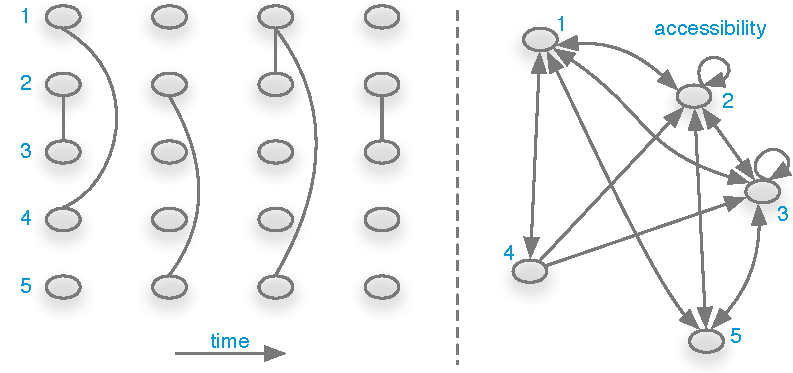
\includegraphics{Temporal_Acessibility_example.pdf}
\caption{A temporal network (left panel) and its accessibility graph (right panel).
The network is taken from Figure~\ref{fig:temporal_network_principle}.
Only nodes 3 and 4 have self loops in this example.
Note that even though the temporal network is undirected, its accessibility graph is directed (edge (4,2) is unidirectional).}
\label{fig:temp_acc_example}
\end{center}
\end{figure}

Before doing so, we have to point out that the identity matrix $\mathbf{I}$ on the right-hand side of Equation~\eqref{eq:temporal_accessibility} is an artifact of the introduced memory.
This does not make a huge difference for undirected networks, as we have discussed for the static case in Section~\ref{sec:unfolding_static}.
A similar argument can be used in the temporal case, since there is always a path from a node back to itself after 2 contacts at different time steps.
Consequently, whenever an edge between two nodes appears twice, both nodes have a self loop in the accessibility graph.
In directed networks, the identity matrix could indeed cause discrepancy from the real accessibility matrix.
Nevertheless, this discrepancy is small, since the contribution of the diagonal is small compared to the total number of elements in $\mathcal{P}_n$.
This holds in particular, since accessibility matrices are in general not sparse.
Therefore, the deviation is ignored throughout this work.

It is important to emphasize that the index $n$ in Equation~\eqref{eq:temporal_accessibility} does not have the meaning of a length of a shortest path as in the static case.
In fact, $n$ measures the \emph{duration} of a path.
Therefore, unfolding an accessibility graph does not yield a shortest path length distribution, but rather the distribution of shortest path durations.
Even if a particular temporal network might be a small-world network in the topological sense -- say it still takes only a few edges to traverse the whole system -- the traversal could take a long time.
In general, even a small world network could be a ``slow world'' network. 

Finally, it should be noted that the accessibility graph of a temporal network is in general directed, even if every snapshot is an undirected network.
Figure~\ref{fig:temp_acc_example} shows the accessibility graph of the network used in Figure~\ref{fig:temporal_network_principle}.
As the figure demonstrates, the accessibility graph is directed, eventhough the underlying temporal network is undirected.
This property reflects the ``arrow of time'' in temporal networks.
In addition to that, the accessibility graph does not show global transitivity as opposed to the static case (compare to Figure~\ref{fig:access_static}).
In our example, the existence of the paths $4\rightsquigarrow 2$ and $2\rightsquigarrow 3$ does not imply that $4\rightsquigarrow 3$, as it would be in the static case.
 
\subsection{Representative sample / characteristic time scale}
We come back to the the findings of Section~\ref{sec:representative_sample}, where we determined the typical timescale of the livestock trade network using data-driven methods.
Thus, we apply the unfolding accessibility method to the livestock trade network dataset, i.e. we take more and more snapshots to obtain information about the path density.
From the derivative of the path density we obtain the distribution of shortest path durations in the network.
The result for the livestock trade network is shown in Figure~\ref{fig:plos_unfolding}.
%
\begin{figure}[htb]
\begin{center}
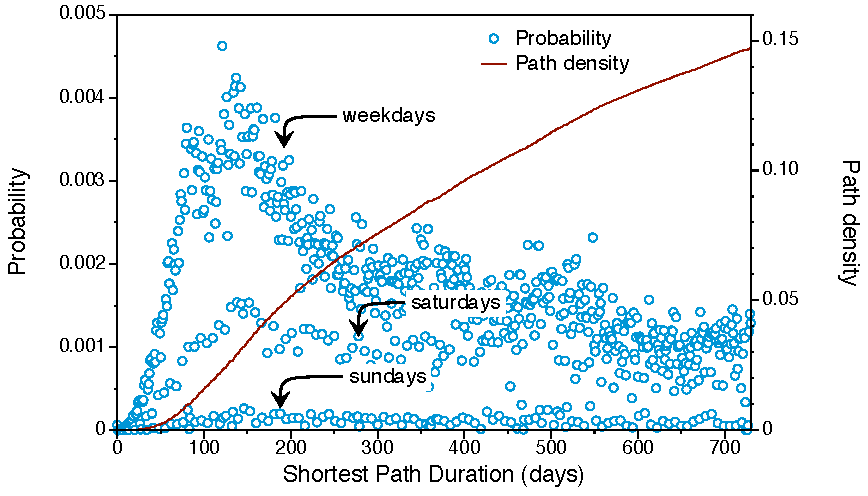
\includegraphics{Plos_Unfolding.pdf}
\caption{Path density (red) and distribution of shortest path durations (blue) for the pig trade network.
Multiples of weekdays are generally more likely for shortest path durations, since trade is less on sundays and almost absent on sundays.}
\label{fig:plos_unfolding}
\end{center}
\end{figure}
%
The path density is relatively low along the whole observation period, since the pig trade network is directed.
We have seen in Section~\ref{sec:components_ranges} that even the static network representation is fragmented, i.e. the largest strongly connected component is relatively small.
Since the components of the aggregated network define an upper bound for the components in the temporal view, the temporal path density is confined.

Although the shortest path durations show a broad distribution, Figure~\ref{fig:plos_unfolding} shows that this distributions has a global maximum.
It follows that there is a typical timescale in the system, which is in the region of 180~days.
This means that the typical spreading time of any process on the network is in the order of 100~days.
In fact, this timescale is a manifestation of the underlying process taking place on the network, i.e. the production of livestock pigs.
The time scale detected in Figure~\ref{fig:plos_unfolding} is in agreement with the representative sample found using a data-driven approach as reported in Figure~\ref{fig:Plos_S1} (see Section~\ref{sec:representative_sample}).
We conclude that the representative sample size of 180~days can be explained by the characteristic time scale of the system.

%
\begin{figure}[htb]
\begin{center}
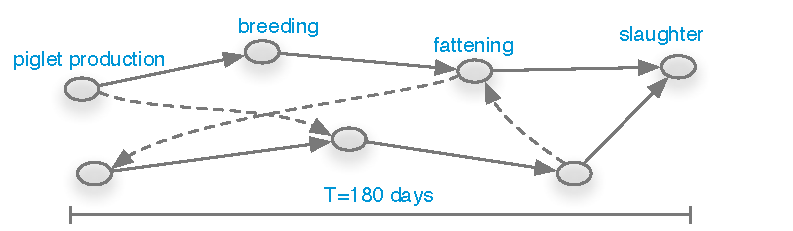
\includegraphics{Pork_production_chain.pdf}
\caption{Simplified representation of the pig trade network.
The system consists of multiple distinct production chains plus a certain degree of ``random'' trade connections indicated by the dashed arrows.
The total production time of one single production chain is 180~days, which defines its temporal diameter.}
\label{fig:pork_production_chain}
\end{center}
\end{figure}
%
The underlying process follows a production chain as shown in Figure~\ref{fig:pork_production_chain}.
As the figure illustrates, the pig trade network is a union of many disjoint production chains.
In addition, there a trade links in the network, which do not follow the exact production path and are shown as dashed lines in Figure~\ref{fig:pork_production_chain}.
The timescale of each production chain is strictly determined by the biological properties of pig production.
Most pigs are slaughtered in the age of 180~days.
This period defines the \emph{temporal diameter} of the production chain, which gives an explanation for the existence of a typical time scale observed in Figure~\ref{fig:plos_unfolding}.

\subsection{Causal fidelity}\label{sec:causal_fidelity}
A large number of tools and measures has been developed for static networks and some of which were reported in Section~\ref{sec:network_theory}.
For this reason, temporal networks are often aggregated and treated as static networks.
The penalty of such an approximation is that it allows for paths that do not follow a causal sequence of edges.
In other words, the most fundamental difference between a temporal network and its aggregated approximation lies in the difference between the number of possible paths.
The question is how closely does an aggregated network reproduce the path properties of the temporal network.
In order to quantify this ability, we define the measure of \emph{causal fidelity}
\begin{equation}\label{eq:causal_fidelity}
c=\frac{\rho (\mathcal{P}_T)}{\rho (\mat{P}_T)} ,
\end{equation}
where $\rho (\mathcal{P}_T)$ is the path density of the fully unfolded temporal accessibility graph and $\rho (\mat{P}_T)$ its static counterpart.
The causal fidelity lies in the range $0\leq c \leq 1$.
Large values of $c$ indicate that an aggregation of the temporal network gives a good approximation of the temporal system from a causal point of view.
A low value of $c$ implies that most paths in the static network can not be taken in the temporal system, since their edges do not causal sequences.
Consequently, temporal networks with small causal fidelities should not be treated as static systems.

If a temporal network with low causal fidelity is treated as a static network, any spreading process on the system would be significantly overestimated.
The ability to quantify this error is an important contribution to risk assessment in epidemiology.

For the pig trade network, we measure $2,202,369,723$ paths in the static network and only $1,575,699,560$ paths in the temporal network.
Hence, the causal fidelity of this network is
\begin{equation}\label{eq:pig_causal_fidelity}
c=\frac{1,575,699,560}{2,202,369,723}\approx 0.715.
\end{equation}
Thus, about $72$~\% of the paths exist in both network representations.
We state that the aggregated network captures the causality of the system sufficiently well. 

It should be noted that Equation~\eqref{eq:causal_fidelity} computes the causal fidelity for the fully unfolded accessibility graph $\mathcal{G}^*_{n=T}$.
In principle, the causal fidelity can also be computed for intermediate steps of the unfolding procedure.
This approach can be used in order to quantify the size of a minimal aggregation window that guarantees for a sufficiently large causality in the approximation.

\subsection{Randomization techniques}\label{sec:randomized_models_tvg}
In order to assess the strength of topological and temporal correlations in the network, we make use of randomized models of the original dataset to remove specific correlations.
A standard procedure to remove correlations on a \emph{static} network is randomizing its edges.
This procedure keeps the degree sequence constant and is similar to the configuration model.
Time as an additional dimension in temporal networks requires for a large number of randomizing procedures in order to systematically remove correlations.
We briefly report, how different randomization procedures affect the temporal network $\mathcal{G} $ and its aggregated counterpart $G$.
Random models for temporal networks have been introduced in \citep{Pan:2011dga,Holme_review}.
We use these models and translate them into our formalism based on the adjacency matrix sequence of a temporal network, i.e.
\begin{equation}\label{eq:AdMatrixSequence2}
\mathcal{A}=\mat{A}_1,\dots ,\mat{A}_T.
\end{equation}
The following random models are applied to our dataset:
%
\paragraph{RE -- randomized edges\color{Cayenne}{.}}
Each snapshot in sequence \eqref{eq:AdMatrixSequence2} is randomized according to the following procedure.
Choose two edges $(u,v)$ and $(w,x)$ in the network randomly.
If the edges are disjoint, i.e. $u\neq w$ and $v\neq x$, then swap the nodes $v$ and $x$.
Thus, the new edges are $(u,x)$ and $(w,v)$.
This procedure is repeated until every edge in the original network has been swapped.

The RE model is similar to the configuration model mentioned in Section~\ref{sec:BA_model}.
It keeps the degree sequence constant and removes higher order topological correlations from the network.
Affected are properties as the clustering coefficient or generally any specific subgraph in the original system.
In the context of the pig trade network, these subgraphs are the production chains illustrated in Figure~\ref{fig:pork_production_chain}.
Since the RE model places new edges almost randomly, it adds a significant amount of mixing to the network.
Consequently, a large deviation between the original network and the RE network indicates that the initial system was not well mixed.
Note that the RE model does explicitly affect \emph{topological} correlations.

The RE procedure also affects the aggregated network.
Since new, random edges are placed for every snapshot, the new aggregated network can have a significantly larger edge density than the original aggregated network.
Models for the removal of temporal correlations are discussed next.

\paragraph{TR -- time reversal\color{Cayenne}{.}}
The TR model considers the network evolution backwards in time.
Using the adjacency matrix sequence, the TR procedure yields a new sequence of adjacency matrices given by
\begin{equation}\label{eq:TR_secuence}
\mathcal{A}^{-1}=\mat{A}^\top _T, \dots ,\mat{A}_1 ^\top,
\end{equation}
i.e. every matrix in the sequence is transposed and the order of the sequence are reversed.
Transposing the matrices reverses the direction of all edges in a network.
This step is of course obsolete in undirected networks.

If the path density of a temporal network is significantly affected by time reversal, the network has a significant temporal directionality.
This behavior occurs in particular, if the activity of the network monotonously changing over time, e.g. during a growing or shrinking process.
The TR procedure also reverts the aggregated network, i.e. $G_{\mathrm{TR}}=G^{-1}$.

\paragraph{GST -- globally shuffled times\color{Cayenne}{.}}
The occurrence time of each snapshot of the network is placed randomly.
This can be directly implemented using a random order of the matrix sequence, i.e.
\begin{equation}\label{eq:GST_sequence}
\mathcal{A}_\mathrm{GST}=\mathrm{shuffle}(\mathcal{A}) ,
\end{equation}
where the function $\mathrm{shuffle}(X)$ returns a random order of a sequence $X$.
Although this model keeps the single snapshots constant, it explicitly removes \emph{temporal} correlations in the system.
These correlations manifest themselves in bursty behavior, such as a broad distribution of waiting times.
Consequently, waiting times in the system are strongly affected by the GST model.

Since the GST procedure does not affect the topology of the snapshots, the aggregated network remains unchanged, $G_\mathrm{GST}=G$.

\paragraph{LST -- locally shuffled times\color{Cayenne}{.}}
Instead of placing snapshots of the system at random times, the LST model randomly assigns the occurrence times of single \emph{edges}.
This model is very similar to the GST model.
It can be efficiently implemented using an edge centric network representation as discussed in Section~\ref{sec:tvg_viewpoints}.
To give an example, a particular edge $(u,v)$ could be present at times $t_1$ and $t_5$, i.e. using the edge occurrence function $\mathcal{I}((u,v))=t_1,t_5$.
The LST model assigns new occurrence times, but keeps the number of edge occurrences constant, e.g. $\mathcal{I}_\mathrm{LST} ((u,v))=t_3,t_{12}$.

As the GST model, the LST model does not change the aggregated network so that $G_\mathrm{LST}=G$.

\paragraph{RT -- random times\color{Cayenne}{.}}
The RT model uses the aggregated network $G=(V,E)$ and places random subsets of $E$ as snapshots.
As the GST and LST models, the RT procedure removes temporal correlations from the system.
In addition to that, the random occurrence of edges mimics a contact rate between the nodes in the system.
The RT model is therefore similar to a weighted static representation of the system.
Different rules for the number of edges per snapshots are possible:
First, every time step could be treated equally so that the number of edges is constant over all snapshots on average.
Second, the distribution of edge densities over all time steps remains constant.
The first and the second variant correspond to the $G_{N,p}$ and the $G_{N,m}$ ensembles known from \ER networks, respectively.
Consequently, the third variant can more efficiently implemented, since the number of edges is known from the beginning.

Since the RT model removes bursty behavior in every path of the network, it affects \emph{scheduled} systems in particular.
These are systems, where paths follow strict time schedules and the systems are temporally sparse.
This is typical for production networks such as the livestock trade network discussed in this thesis.
Being related to a weighted static network, the RT model does not affect the topology of aggregated network, so that $G_\mathrm{RT}=G$.
It should be noted that due to the impact of chance, a small number of edges might not be chosen in the snapshots of $E$.
Consequently, $G_\mathrm{RT}\approx G$ up to negligible statistical fluctuations.
%
%\paragraph{Summary of methods\color{Cayenne}{.}}
A summary of the used randomization models is shown in Table~\ref{tab:random_models}.
\begin{table}[htb]
\sffamily
\begin{center}%\centering
\caption{Effects of the different randomization models.
}
\begin{tabular*}{\hsize}{@{\extracolsep{\fill}}cl}
\hline
Model & Effects\\
\hline \hline
\multirow{3}{*}{RE} & addition of topological mixing\\
& removes specific topological subgraphs\\
& static network changed\\
\hline
\multirow{2}{*}{TR} & reverts arrow of time\\
& static network reversed\\
\hline
\multirow{4}{*}{GST} & graph-centric\\
&conserves bursty occurrence of edges\\
& homogenizes edge occurrences over the observation time\\
& removes characteristic time scales\\
& static network unchanged\\
%
\hline
\multirow{4}{*}{LST} & edge-centric \\
& conserves bursty occurrence of edges\\
& homogenizes edge occurrences over the observation time\\
& removes characteristic time scales\\
& static network unchanged\\
%
\hline
\multirow{2}{*}{RT} & removes bursty occurrence of edges\\
& static network (almost) unchanged \\
\hline \hline
\end{tabular*}
\label{tab:random_models}
\end{center}
\end{table}

\subsection{Temporal and topological mixing patterns}
In order to reveal temporal and topological correlations in the livestock trade dataset, we apply the randomization techniques from the previous section to the network.
Every deviation from the original dataset hints to a particular correlation in the network.
Figure \ref{fig:randomized_hit} shows the path density for the original dataset and for the randomized versions.
The red curve shows the original network.
\begin{figure}[htb]
\begin{center}
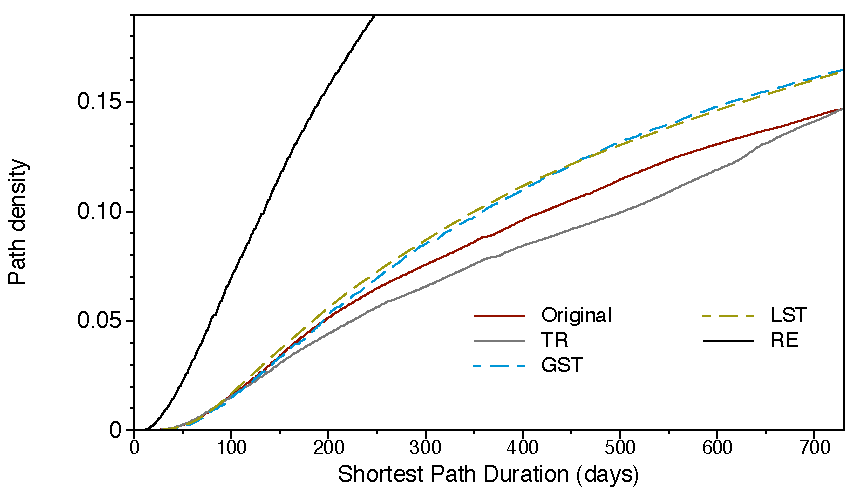
\includegraphics{Plos_Unfolding_randomized.pdf}
\caption{Path densities of randomized networks of the livestock trade dataset.
Black points represent the original dataset.
The randomization models are TR -- time reversal, GST -- globally shuffled times, LST -- locally shuffled times, RE -- randomized edges and RT -- random times.
}
\label{fig:randomized_hit}
\end{center}
\end{figure}

As the figure demonstrates, time reversal has a measurable effect for shortest path durations larger than about 100~days (grey line).
Overall, the path density is lowered over a wide range of times.
This shows that causal chains are less frequent, when the network is traversed backwards in time.
This feature reflects the temporal directionality of the underlying production chain.
In addition, the lower path density implies that a significant fraction of paths with duration between 100 and 700 days are ``single events'', i.e. they do not form highly frequented lanes.
More specifically, a single event path is a causal chain of edges, where each edge has only few occurrence times.
These structures are particularly sensitive to time reversal. 

The role of temporal correlations can be examined using time shuffling models.
In Figure~\ref{fig:randomized_hit}, the GST and LST models are shown as dashed blue and red lines, respectively.
Both lines show no significant differences from each other, indicating that the application of both procedures has a similar effect.
The figure shows that time shuffling significantly increases the path density is over a large period of shortest path durations.
Since the GST and LST models remove temporal bursty behavior from the system, we conclude that the node waiting times restrict the number of paths in the original system. 

The random times (RT) model removes scheduling from the network.
The consequence is a significant increase of the path density (green line).
An explanation for this behavior is that most paths in the system show a bursty behavior.
It should be noted that the path density of the RT model almost approaches the path density of the aggregated network -- i.e. $\rho (\mat{P}_T)\approx 0.206$ -- in this case study.
% RT_path_density = 2202369723/10710180100
This high path density is caused by the relatively high activity of the system.
As we have observed in Section~\ref{sec:representative_sample}, about 10~\% of the edges are active every day.

It is a salient feature of this dataset that edge randomization (RE model, orange line) considerably increases the overall path density.
The reason is that the underlying production chain strongly determines the network.
As we have seen in Figure~\ref{fig:pork_production_chain}, the livestock trade system basically consists of a number of disjoint production chains as basic units.
These basic units are interconnected by few ``random'' links.
As a consequence, the whole system is by far not well mixed.
Applying the RE model to the network provides strong mixing of the trade contacts.
This mixing results in a large number of possible paths, also the aggregated network has a path density of $\rho (\mat{P}_T)\approx 0.449$, which is more than twice as much as the original data.

In summary, the underlying production chain of the livestock trade network is ubiquitous in the path structure of the network.
The most salient feature in this context is the poor topological mixing of the network.
Another striking feature is that bursty trade transactions seem to dominate the traversal of the system.
Temporal correlations and temporal directionality play a role, but these features are not as striking as mixing and scheduling.

\subsection{Further case studies}
%
\begin{SCfigure}
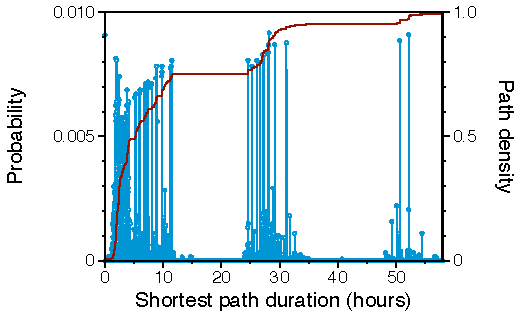
\includegraphics{113-Sociopatterns.pdf}
\caption{Unfolding accessibility of a conference contact network.
The fast saturation behavior and the high maximum of the path density suggest a high degree of mixing in this system.}
\label{fig:113}
\end{SCfigure}
%
In order to demonstrate the capability of the unfolding accessibility method for the study of other systems, we apply the methods discussed before to two other datasets:
First, a network of face-to-face contacts measured during a conference and second, a network of sexual contacts between prostitutes and their customers measured via an online rating platform for escorts.
Both networks are undirected.
As the pig trade network, both networks are possible substrates for the spread of infectious diseases -- in this case, droplet transmitted diseases (e.g. flu) and sexually transmitted diseases, respectively.
Both datasets are available online.
Further information on the conference network is found in \citep{isella2011,sociopatterns.org} and the sexual contact network is analyzed in \citep{Rocha_pnas}.

Figure \ref{fig:113} shows the path density and the distribution of shortest path durations for the conference contact network.
The observation period of three days separated by periods of weak interaction (nights) are clearly resolved in the figure.
Overall, this network is particularly active.
This is reflected by the relatively high maximum path density of $\rho (\mathcal{P}_T) \approx 0.99$, i.e. almost all possible paths are traversed within the observation period.
%
\begin{figure}[h!]
\begin{center}
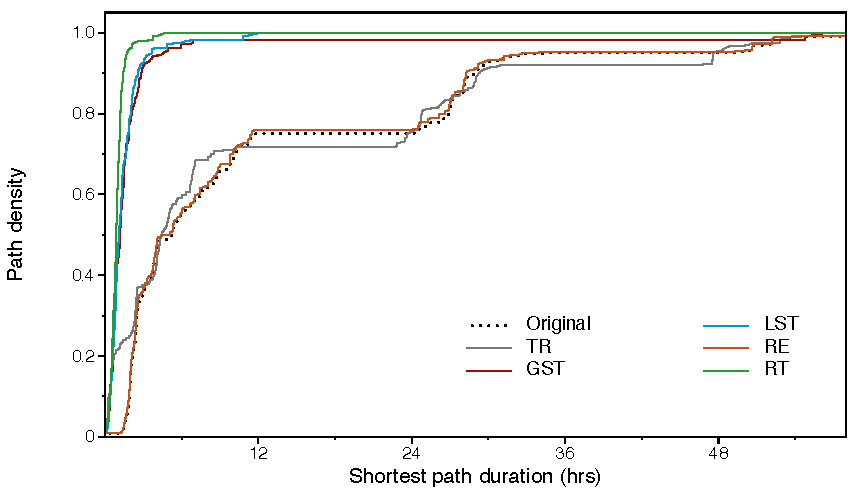
\includegraphics{Sociopatterns_Randomized.pdf}
\caption{Path densities of randomized networks of the conference contact network.
Removing temporal correlations (GST, LST, RT) removes periods of no activity (nights) from the network and significantly decrease the characteristic time scale and the temporal diameter.}
\label{fig:113_random}
\end{center}
\end{figure}
%
As we have discussed in Section~\ref{sec:conceptual_problems}, the high overall path density indicates that there exists a giant causally connected component in the system.
However, the question of mutual connectivity cannot be answered in detail using the accessibility graph alone.

It can be read immediately from the path density that within the first day of the conference, more than 70~\% of all possible paths have been traversed.
The median of the shortest path duration distribution is reached within the first 6~hours.
Thus, we conclude that 6~hours is a typical timescale for spreading processes in this system.

Following Section~\ref{sec:causal_fidelity}, we use Equation~\eqref{eq:causal_fidelity} and compute the causal fidelity of the conference network.
As can be conjectured from the high path density, the causal fidelity attains the relatively high value $c\approx 0.99$.
This implies that an aggregated network gives a good approximation of the real system from the causal point of view.

In order to assess the mixing properties of the conference contact network, we apply the randomization techniques of Section~\ref{sec:randomized_models_tvg} to the dataset.
The result is shown in Figure~\ref{fig:113_random}.
As the figure demonstrates, time reversal (TR) and randomizing edges (RE) do not significantly change the behavior of the path density.
The small effect of the RE model implies that the system is already (topologically) well mixed.
Also the time reversal invariance can be attributed to the strong mixing and the high activity of the system.
Note that both models preserve the plateaus caused by night-times.

Removing temporal correlations has a similar effect for the GST, LST and RT model.
All three models show a steep increase of the path density and within only a few hours the maximum path density is reached.
This effect originates from the fact that all three models remove the night periods from the system and thus the edge activity is distributed over the whole time period.

We now focus on a network of sexual contacts between escorts and customers over a time span of 6 years.
Figure~\ref{fig:sexual_contacts} shows the unfolding path density of the temporal network.
%
\begin{SCfigure}
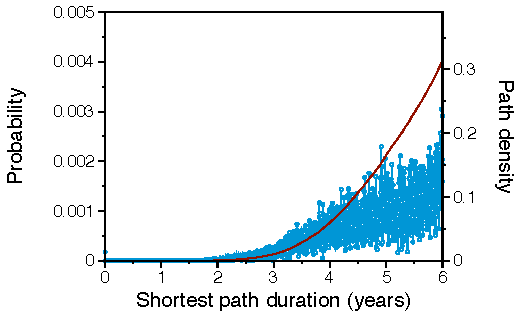
\includegraphics{Sexual_Contacts.pdf}
\caption{Path density and shortest path duration distribution for a network of sexual contacts.
Despite the long observation period, the path density does neither saturate nor it reveals a characteristic time scale.}
\label{fig:sexual_contacts}
\end{SCfigure}
%
The accessibility graph is very sparse during the first 2 years of observation.
Even after the 6 years it remains difficult to extrapolate the path density and estimate a saturation behavior.
Hence, no characteristic time scale can be observed during the observation period.
%
\begin{figure}[htb!]
\begin{center}
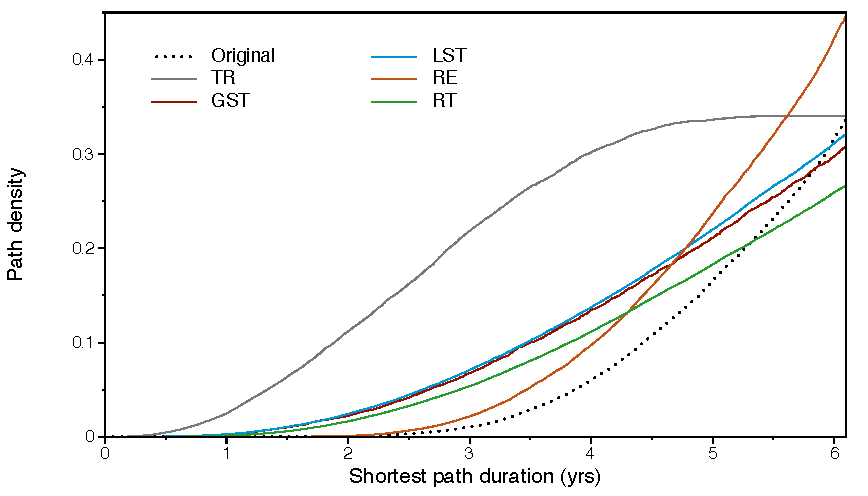
\includegraphics{Sexual-randomized.pdf}
\caption{Path densities of randomized networks of the sexual contact network.
The system is not well mixed (RE model, orange) and not time reversal invariant (TR model, grey).
The path density of the TR model indicates that the data density is monotonously increasing in the original data.}
\label{fig:sexual_randomized}
\end{center}
\end{figure}
%
Although the dataset does not give clear results, we can state that any disease takes more than 2~years to infect a finite fraction of the network.
The results are also valuable for further studies, since we have demonstrated that longer observation periods are needed in order to measure the characteristic spreading time in this system

In addition, the causal fidelity of this network is $c=0.38$.
This clearly provides support for treating the system from a temporal perspective -- as done in \citep{Rocha_pnas} -- since a static approximation would significantly overestimate the size of any disease outbreak.

Finally, the path densities of randomized models of the sexual contact network are shown in Figure~\ref{fig:sexual_randomized}.
A salient feature of this figure is that time reversal significantly changes the behavior of the path density (grey line).
In fact, the edge density of the system increases monotonously over time and it has been shown that this circumstance alone can cause this behavior in the supplementary information of \citet{Lentz:2013PRL}.
The impact of removal of temporal correlations -- i.e. GST (red), LST (blue) and RT (green) model respectively -- can be explained in a similar fashion.
All of these procedures homogenize the edge density over time resulting in a systematic increase of the path density.
Due to the overall sparsity of edge data, the RT model places relatively sparse networks as snapshots in this case.
This impedes the formation of causal chains.
Therefore, the path density of the RT model is slightly smaller than in the case of the time shuffling models.

Interestingly, the path density of the time shuffling models fall below that of the original data in the long term.
It is not clear, whether this can be attributed to the increasing edge density or whether it reflects an intrinsic property of this system.
A longer dataset would be needed in order to answer this question. 

As it was the case for the livestock trade network, the sexual contact network is not well mixed.
This is measured in terms of a strictly higher path density in the RE model (orange line) than it was in the original data.

        \chapter{Conclusion}
In this thesis we have examined the role of paths for the spread of infectious diseases on networks.
The importance of paths in the context of epidemiology has been demonstrated for the case of static networks and was then carried over to the temporal case.
As a central result, we have introduced the unfolding accessibility method for temporal networks in order to analyze the path structure of these systems.

Concerning the spread of infectious diseases on complex networks, detailed knowledge of the dynamical aspects of disease transmission is not known in most real-world scenarios.
It turns out however that the pure topology of contact patterns is of major importance in this context.
In contrast to the infection parameters of most diseases, the contact structures can be measured to great detail for a large number of real-world systems.
Although these contact structures form complex networks, which exhibit a wealth of properties in most cases, it turns out that the structure of paths in these systems defines the domain for any spreading process.
On the one hand, the range of a node defines an upper limit for the size of disease outbreaks.
On the other hand, the path structure of the whole system can be mapped onto the accessibility of the network.

In this thesis, we have analyzed the impact of two particular attributes of \emph{static} complex networks on the properties of their paths.
As a generic complex network, we analyzed the properties of a livestock trade network in Germany in detail.
Among other features, the network exhibits a giant component and a significant modular structure.
The existence of a giant component strikingly affects the spreading potential of the network nodes.
Whenever a network is close to its critical point, its nodes can be divided into two disjoint risk classes.

A weaker restriction on the path-connectivity between subgraphs is the concept of modules, i.e. densely connected subgraphs being sparsely interconnected.
These structures have a relatively weak effect on the outbreak size.
This is particularly true for meta population networks, where nodes are permeable for disease spread, if they are not fully recovered.
However, a modular network is likely to show a significantly delayed outbreak peak.
This result could be useful for the implementation of counter measures, since it does not depend on a particular partitioning of a network, but only on the fact that the network is to a certain extent modular.

Special emphasis should be placed on the methods introduced for the analysis of \emph{temporal} networks, i.e. systems where the occurrence of edges varies over time.
These systems are particularly challenging due to the importance of causality for any path on a temporal network.
We have introduced a novel method to obtain the accessibility graph of a temporal network.
We believe that the definition of accessibility of temporal networks contributes a key element for a theoretical framework for the macroscopic analysis of temporal networks, because it maps the whole causal path structure of the system onto a single mathematical object.
Moreover, we have introduced \emph{unfolding} accessibility as a novel formalism for the evaluation of shortest path durations in temporal networks.
This approach is able to reveal characteristic timescales for the traversal of temporal networks.
Knowledge of these timescales is of fundamental importance for the estimation of spreading times.

In addition to the above, the accessibility graph of a temporal network can be compared to its aggregated, static counterpart.
Using this concept, we have defined the novel measure of \emph{causal fidelity}, which quantifies the goodness of the static approximation of a temporal network from the causal point of view.
This measure is of major importance, since due to the lack of established temporal network analysis tools, a static approximation can provide useful insights into the real system.
%This measure is of major importance, since static network analysis provides a huge toolbox for quantifying network properties. 
%Since there is no such toolbox for temporal networks yet, the static approximation of a temporal network can give useful insights into the real system.
On the other hand, temporal networks with low causal fidelities should be analyzed with care, when static network tools are used.
In particular, a low causal fidelity implies that disease outbreaks are systematically overestimated in the static approximation.


\paragraph{Outlook\color{Cayenne}{.}}
The generalization of the \emph{clustering coefficient} known from static networks (see equation \eqref{eq:clustering_coefficient}) can be done in a straightforward manner using the adjacency matrices of network snapshots.
Thus, the temporal clustering coefficient reads $C_{ijk}=\text{tr} (A_{i}A_{j}A_{k})/( \sum_{\mu,\nu\in\{i,j,k\}:\mu<\nu}\left[\sum _{\mu \nu }\left(A_{\mu}A_{\nu}\right)-\text{tr}\left(A_{\mu}A_{\nu}\right)\right])$.
The clustering coefficient has to be computed for all snapshot triples with indices $i<j<k$ and gives a 3-dimensional object.
This object can be contracted to a clustering matrix $\mat{C}$ with elements $c_{j-i,k-j}$ and a clustering vector $\mat{c}$ with elements $c_{k-i}$.
The former gives information about the node waiting times in closed triangles and the latter measures the total time of closed triangles in the network.

Although accessibility is a fundamental building block for the understanding of temporal networks, the development of a macroscopic theory of temporal networks is still in its infancy.
A promising approach would consist in mapping temporal network properties onto some static network image and analyze the latter instead.
Besides the obvious temporal nature of most network measures in temporal networks, the difficulty in such an approach lies in conceptual problems such as the degeneration of connected components.
These problems are mostly attributed to the non-transitivity of paths in temporal networks.
Hence, finding the transitive part of an accessibility graph could prove to be useful.
The author suggests to quantify \emph{transitivity} as follows: the transitivity matrix $\mathbf{T}=\mathcal{P}_T\circ \mathcal{P}_T ^2$ contains the transitive edges of the accessibility graph ($\circ $ denotes the Hadamard product).
This measure could help to identify transitive paths in temporal networks and facilitate the generalization of other concepts of static network analysis.







    %\backmatter
        \appendix
        %\documentclass[openright,twoside,headsepline]{scrbook}
%\usepackage[applemac]{inputenc}
%\usepackage{graphicx,xcolor,hyperref} % obsolete in HU-diss
%\usepackage[round,authoryear]{natbib}
%\setlength\bibhang{2em} 
%
%
%\KOMAoptions{numbers=noenddot}
\usepackage{amsmath,amssymb,amsfonts,amsthm,epigraph,scrpage2}
\usepackage[ngerman,english]{babel}
\definecolor{Cayenne}{rgb}{0.502,0.0,0.0}
\definecolor{Steel}{rgb}{0.4,0.4,0.4}


%\setcounter{secnumdepth}{3} % sub subsections numbering
%\setcounter{tocdepth}{3} % subsubsections inTOC

\usepackage[format=plain,singlelinecheck=false, font={sf,small},labelfont={bf,color=Steel}]{caption}
\DeclareCaptionLabelSeparator{cayenne_period}{\textcolor{Cayenne}{.} }
\captionsetup{labelsep=cayenne_period}

% Colors
\addtokomafont{chapter}{\color{Steel}}
\addtokomafont{section}{\color{Steel}}
\addtokomafont{subsection}{\color{Steel}}
\addtokomafont{subsubsection}{\color{Steel}}
\addtokomafont{paragraph}{\color{Steel}}

\addtokomafont{pagehead}{\color{Steel}}
\renewcommand{\pnumfont}{\color{Steel}} 
\addtokomafont{headsepline}{\color{Steel}} 
\pagestyle{scrheadings} 

%\makeatletter % dot after sections and all below
%\let\std@sect\@sect
%\def\@sect#1#2#3#4#5#6[#7]#8{\std@sect{#1}{#2}{#3}{#4}{#5}{#6}[#7.]{#8\color{Cayenne}{.}}}
%\makeatother

\usepackage[leftcaption]{sidecap} % inner, outer,left,right
\sidecaptionvpos{figure}{t}

% Papiergr��e
%\setlength{\paperwidth}{24cm}
%\setlength{\paperheight}{17cm}
%\recalctypearea
%\usepackage{geometry}

%% Flattersatz
%\usepackage[document]{ragged2e} % Flattersatz
%\setlength{\RaggedRightParindent}{1em} % evtl. parskip


%% Sans Serif
%\usepackage{cmbright}
%\renewcommand{\familydefault}{\sfdefault}
%% Palatino
%\usepackage[sc]{mathpazo}
%\linespread{1.05}         % Palatino needs more leading (space between lines)
%\setkomafont{sectioning}{\normalcolor\bfseries} % Kapitel�berschriften

%%% Kapitel�berschriften: Mit gro�en Zahlen
%\usepackage{titlesec}
%\titleformat{\chapter}[display]
%{\bfseries\Large}
%{ %\Huge\textsc{\chaptertitlename} % f�r das Wort 'Kapitel'
%\hfill\fontsize{120}{70}\selectfont\color{lightgray}\textbf{\thechapter}}
%{-2ex}
%%{\filleft\fontsize{50}{70}\selectfont\scshape} % Kapit�lchen oder...
%{\filleft\fontsize{50}{70}\selectfont\textbf} % ...oder keine Kapit�lchen
%[\vspace{0ex}]
%
%%%% Part�berschriften
%\titleformat{\part}[display]
%{\bfseries\Large}
%{ %\Huge\textsc{\chaptertitlename} % f�r das Wort 'Kapitel'
%\hfill\fontsize{120}{70}\selectfont\color{lightgray}\textbf{\thepart}}
%{-2ex}
%{\filleft\fontsize{50}{70}\selectfont\scshape} % Kapit�lchen oder...
%%{\filleft\fontsize{50}{70}\selectfont\textbf} % ...oder keine Kapit�lchen
%[\vspace{0ex}]


\newcommand{\ER}{Erd\H{o}s-R\'enyi }
\newcommand{\BA}{Barab\'asi-Albert }
\newcommand{\mean}[1]{\left< #1 \right>}
\newcommand{\abs}[1]{\left| #1 \right|}
\newcommand{\norm}[1]{\lVert#1\rVert}
\newcommand{\mat}[1]{\mathbf{#1}}
\newcommand{\tgraph}{\mathcal{G}}

\theoremstyle{definition} % non-italic
\newtheorem{annahme}{Annahme} % braucht amsthm
\newtheorem{definition}{Definition}
\newtheorem{theorem}{Theorem}
\newtheorem{satz}{Satz}
\newtheorem{frage}{Frage}
%\input{watermarks/watermark.tex}
\DeclareMathOperator{\nnz}{nnz}

% + Graphicspath nach begin document

%
%
%
%\begin{document}
%\graphicspath{{/Users/lentz/Documents/GitHub_locals/Thesis/images/}}
%\tableofcontents

\chapter{Appendix}

\section{Network implementation}\label{sec:implementation}
In order to efficiently implement networks and their analysis on a computer, it is necessary to use data structures adjusted to these problems.
A short and transparent introduction to data structures and algorithms is in the book of \citeauthor{algorithm_design} \citep{algorithm_design}.
In this section, we discuss some essential data structures appropriate for network analysis and give a brief description of fundamental algorithms.
The purpose of this section is not to list different algorithms and source code, but rather to sketch the basic ideas behind the data structures and algorithms.
For source code of data structures and algorithms, the reader is encouraged to the lecture of \citep{algorithm_design} and \citep{Merali:2010ih}.

\paragraph{Matrix implementation\color{Cayenne}{.}}
To begin with, we consider the implementation of adjacency matrices as introduced in section \ref{sec:network_matrices}.
Matrices can be seen as a \emph{graph centric view} on the network, since they map the whole network topology onto a single object.
Adjacency matrices are by definition square matrices.
Their entries are either $0$ or $1$, and can take any floating number value for weighted networks.
In this work, we neglect negative edge weights.
The number of nodes in most complex network datasets is relatively large. 
Starting with small networks (100 nodes, conference contacts \citep{isella2011}), complex networks can be gigantic (0.5 billion nodes, twitter tweeds \citep{Yang:2011}).
Note that the size of the adjacency matrices scales with the square of the networks size, hence large networks intractable for straightforward computer-based matrix analyses.

Nevertheless, there is one feature, that most adjacency matrices of real-world networks have in common:
they are \emph{sparse}, i.e. the vast majority of their entries are zeros\footnote{Typically, the number of edges in the network is of the same order as the number of nodes.}.
Since zeros do not contribute to matrix operations as products or additions, it is reasonable to use data structures ignoring zeros.
These data structures are called \verb"sparse matrices".
Their advantages is (1) they save much memory and (2) computations are faster, because operations with zeros involved are not executed.
Sparse matrix data structures are available in most modern computer languages (e.g. Matlab, Python: \verb"scipy" library, C/C++: \verb"boost" library).
They perform well for all problems based on adjacency matrices, e.g. degree or eigenvector centrality.
However, matrix methods are not suitable for the computation of many other network measures, such as betweenness, closeness or network navigation.

\paragraph{Graph implementation\color{Cayenne}{.}}
The weakness of matrix representations of networks is that it is rather complicated to \emph{traverse} a network using matrices.
A traversal is a procedure like: start at a node, visit all of its neighbors, from each neighbor visit its neighbor and so forth, until there are no more new nodes to traverse.
This is a searching process.
These processes are used in many implementations of graph theoretic methods.

An alternative implementation to the adjacency matrix is the \verb"adjacency list".
It stores the neighbors of every node and is implemented in terms of a linked list.
Adjacency lists can be considered as a \emph{node centric view} on the network, since they capture the horizon/neighborhood of each node.
Using the example network of \ref{fig:simple_digraph}, we get the following adjacency list:
\begin{align*}
1 &\rightarrow 2,3 \\
2 &\rightarrow 4 \\
3 &\rightarrow 2 \\
4 &\rightarrow 2,3 .
\end{align*}
In order to traverse the graph starting at node $1$, we can choose any of the neighbors of $1$ and repeat the process until we have traversed all nodes.
One possible traversal starting at $1$ would be $1\rightarrow 3 \rightarrow 2 \rightarrow 4$.

During a traversal process, one can decide to either exploit the whole neighborhood of a node first and then traverse the next generation or choose a neighbor of every traversed node at every step.
These two essential searching processes are called breadth-first-search (BFS) and depth-first-search (DFS), respectively.
The difference between the two lies in the order of traversed nodes.
Figure \ref{fig:dfs_bfs} shows resulting search trees of the two methods.
Starting at node $1$, the traversal $1\rightarrow 3 \rightarrow 2 \rightarrow 4$ would be found using a DFS-search, while a BFS-search would yield $1\rightarrow 2 \rightarrow 3 \rightarrow 4$.
It should be noted that in general there exist multiple BFS and DFS trees for each starting node. 
%
\begin{figure}[htbp]
\begin{center}
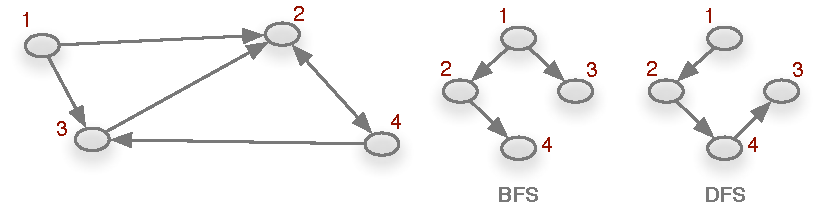
\includegraphics{DFS-BFS.pdf}
\caption{Breadth-first-search and depth-first-search trees in the directed network of fig.~\ref{fig:simple_digraph}. Searches are started at node $1$.}
\label{fig:dfs_bfs}
\end{center}
\end{figure}

Both search algorithms are used in many applications.
BFS is efficient to compute shortest paths in unweighted networks.
With every generation in a BFS tree, the distance from the starting node is incremented by 1, and thus the set of nodes with a certain distance from the starting node can be directly read from the BFS tree (see figure \ref{fig:dfs_bfs}).
Shortest paths in weighted networks can be identified using a the algorithm of Dijkstra \citep{Dijkstra:1959}.
DFS can be used to identify connected components in directed graphs (see next section).

Due to the sparsity of typical adjacency matrices, networks can be efficiently stored as \verb"edge lists".
An edge list is a list of tuples, where each tuple $(u,v)$ is an edge connecting nodes $u$ and $v$.
The edge list of example \ref{fig:simple_digraph} would be
\begin{align*}
&(1,2)\\
&(1,3)\\
&(2,4)\\
&(3,2)\\
&(4,2)\\
&(4,3) .
\end{align*}
Due to their human readable structure, edge lists are a very convenient format to store networks as column wise text files.
Edge lists correspond to an \emph{edge centric view} on a network.
They can be efficiently used for edge randomization and random graph generation.

Implementations of graph structures as discussed above are for example available in the libraries \verb"networkx" (Python), \verb"igraph" (C, Python, R), \verb"Lemon" and \verb"Boost" (C++).

\paragraph{Hard problems\color{Cayenne}{.}}
Although the libraries introduced above provide a huge and efficient toolbox for network analysis, there are still network problems, where no efficient algorithm is known for their exact solution.
In the language of complexity theory, the time to solve these problems scales with the problem size in non-polynomial time.
Problems of this kind can typically be solved exactly only for small system sizes.

Probably the most popular example is the \emph{traveling salesman problem}: a salesman has to traverse a set of cities and thereby choose the order of those cities that minimizes the total distance.
For small problem sizes, it is possible just to try out all possible combinations and find the minimal total distance.
The number of possible combinations, however, grows factorial with the system size, i.e. finding a solution takes $t\propto n!$ for $n$ cities.
In other words, if the problem could be solved for 20 cities in 1 second, it would take 21 seconds to solve it for 21 cities, 7 minutes for 22 cities and 3 million years for 30 cities!

A more exhaustive overview about hard problems is in \citep{algorithm_design} and the references therein.
Generally, heuristic methods have to be used in order to get an approximate solution.
It should be noted that the \emph{maximum clique} problem (see section \ref{sec:PRL}) and \emph{graph partitioning} (see section \ref{sec:network_analysis}, equation \eqref{eq:modularity}) belong to the class of hard problems \citep{brandes2007}.

\section{Subgraphs and maximum modularity}\label{sec:maximum_modularity_subgraphs}
We derive an estimation of the maximum modularity value depending on the number of modules in the network.
The results are derived for a clique of modules, but remain the same for a ring of modules as it is reasonable in finite systems (see below).
In addition, the estimation is also valid for directed networks (see below).

The modularity of a network can be computed using the equation
\begin{equation}\label{eq:mod_undir}
Q=\sum _i \left( e_{ii}-a_i^2 \right),
\end{equation}
where $e_{ij}$ is the fraction of edges pointing from community $i$ to community $j$.
The last term corresponds to the fraction of all edges that are connected to community $i$, i.e.
\[
a_i = \sum _j e_{ij}.
\]
Since the sum over all edge fraction has to be 1, it is $\sum _{ij}e_{ij}=1$.
If a network consists of two modules $x$ and $y$, the fraction of edges in $y$ is
\begin{equation}\label{qmaxbedingung}
y=c-x,
\end{equation}
where the constant $c<1$ is the fraction of all inner module edges.
In general, it is $c=\mathrm{Tr} (e)$.

\subsection{Two modules}
In the case of two communities, the fraction of inter-module-edges is uniquely determined by the fraction of inner-module-edges.

The matrix $e_{ij}$ takes the form
\[
e_{ij}=\left(\begin{array}{cc}x & \frac{1}{2}(1-x-y) \\ \frac{1}{2}(1-x-y) & y\end{array}\right) ,
\]
where $x$, $y$ are the edge fractions \emph{in} communities 1 and 2 and $\frac{1}{2}(1-x-y)$ is the fraction of edges \emph{between} communities 1 and 2.
The corresponding expression for $Q$ is.
\[
Q=x-\left( x+\frac{1-x-y}{2} \right) ^2 +y -\left( y+\frac{1-x-y}{2} \right) ^2 .
\]
This function does not possess a maximum over the total domain, but there is a maximum in the subdomain $0<x<1$, $ 0<y<1$.
Condition \eqref{qmaxbedingung} yields
\[
Q=\frac{1}{2}+2\, cx-2\, x^2-\frac{1}{2}\, c^2+c.
\]
Using condition \eqref{qmaxbedingung} restricts the function to tuples $(x,y)$, where $x+y=c$, which corresponds to a line $y=c-x$.
Thus, we are looking for the maximum along this line using the condition
\[
\frac{\partial Q}{\partial x}=2c-4x=0.
\]
It follows $x=c/2$ and the maximum condition $\partial ^2 Q/\partial x^2 =-4<0$ is satisfied.
Using \eqref{qmaxbedingung} gives the solution
\begin{equation}\label{qmax_xy}
x=\frac{c}{2} , \hspace{0.5cm} y=\frac{c}{2}.
\end{equation}
The corresponding modularity is 
\begin{align*}
Q&=\frac{c}{2}-\frac{1}{4}\left( 1+\frac{c}{2}-\frac{c}{2} \right) ^2 +\frac{c}{2}-\frac{1}{4}\left( 1+\frac{c}{2}-\frac{c}{2} \right) ^2 \\
&= c- \frac{1}{2} .
\end{align*}
The case where a maximum fraction of edges is in the modules and a minimum fraction is between modules is met, if $c\rightarrow 1$.
In this case, the modularity takes its maximum value.
The limit is
\begin{equation}\label{q2limits}
\lim _{c\rightarrow 1} x =1/2, \hspace{0.5cm}\lim _{c\rightarrow 1} y =1/2, \hspace{0.5cm} \lim _{c\rightarrow 1} Q=1/2.
\end{equation}
For the case of two modules, the maximum modularity is found for two equally sized modules of approximate size $1/2$.
The maximum modularity is then $Q=0.5$.
We consider the case of more modules below.

%
\subsection{Arbitrary number of modules}
In the case of more than two modules, all modules can have different sizes in the first place and can be connected among themselves arbitrarily.
The general module-matrix takes the form
\begin{equation}\label{eq:general_module_matrix}
e_{ij}=\left(\begin{array}{ccccc}x_1 &  & \hdots &  & d \\ & x_2 &  &  &  \\\vdots &  & \ddots &  & \vdots \\ &  &  & \ &  \\d &  & \hdots &  & x_n\end{array}\right) .
\end{equation}
All non-diagonal elements are 
\[
d= \frac{1-\text{Tr } (e) }{n(n-1) } = \frac{1-c }{n(n-1) }
\]
with $c\equiv \text{Tr } (e)=\text{const.}<1$.
Thus, the general expression for modularity is
\begin{equation} \label{eq:modumatrix}
Q= c-\sum  _i \left( \sum _j e_{ij} \right)^2 .
\end{equation}
%
We use the above expression for the non-diagonal elements $d$ and compute the expression $\sum _j e_{ij}$ in equation \eqref{eq:modumatrix}.
\begin{equation}\label{eq:sumeij}
\sum _j e_{ij} = e_{ii} + \sum _{j\neq i} e_{ij} = x_i + (n-1) \frac{1-c}{n(n-1)} = x_i + \frac{1-c}{n}.
\end{equation}
%
Now we insert $\sum _j e_{ij}=x_i+\frac{1-c}{n}$ in equation \eqref{eq:modumatrix} and after some algebra we get the general expression for the modularity for networks of the form \eqref{eq:general_module_matrix}:
\begin{equation}\label{eq:Qndim}
Q=c-\sum _i x_i^2 - \frac{1-c^2}{n} = \sum _i x_i -\sum _i x_i^2 - \frac{1-(\sum _i x_i)^2}{n}.
\end{equation}

In order to find the relevant maximum of \eqref{eq:Qndim}, its slope has to vanish along a hyperplane defined by
\begin{equation}\label{qmehrdimbedingung}
\sum _i x_i = c = \text{const.} <1.
\end{equation}
%
Since $c$ is constant, the relevant part of \eqref{eq:Qndim} for the maximum is
\begin{align}
Q_{\text{relevant}}\equiv Q_\text{r}= -\sum _{i=1}^n x_i^2&=-\sum _{i=1}^{n-1} x_i^2- \underbrace{ \left( 
c-\sum _{i=1}^{n-1} x_i \right) ^2 }_{x_n^2} \label{eq:relevant_Q}\\
&= -\sum _{i=1}^{n-1} x_i^2 - c^2 + 2c\sum _{i=1}^{n-1} x_i -\left( \sum _{i=1}^{n-1} x_i \right) ^2. \nonumber
\end{align}
Note that the sum on the r.h.s. runs to $n-1$.
This effectively eliminates the last variable.
The derivative of $Q$ is
\begin{equation}
\frac{\partial Q}{\partial x_i}= \frac{\partial Q_\text{r}}{\partial x_i}=- 2\sum _{i=1}^{n-1} x_i + 2c(n-1)-2 (n-1) \sum _{i=1}^{n-1} x_i.
\end{equation}
%
In order to find a maximum, the derivative has to vanish, i.e.
\begin{align*}
0&=- 2\sum _{i=1}^{n-1} x_i + 2c(n-1)-2 (n-1) \sum _{i=1}^{n-1} x_i \\
&=- \sum _{i=1}^{n-1} x_i + c(n-1) - (n-1) \sum _{i=1}^{n-1} x_i \\
 &= cn-c-n\sum _{i=1}^{n-1} x_i +\sum _{i=1}^{n-1} x_i -\sum _{i=1}^{n-1} x_i\\
 &= cn-c-n\sum _{i=1}^{n-1} x_i .
\end{align*}
It follows
\[
\underbrace{c-\sum _{i=1}^{n-1} x_i}_{x_n} =\frac{c}{n}.
\]
Thus,
\begin{equation}
x_n=\frac{c}{n}.
\end{equation}
Hence, the maximum of $Q$ is obtained, if all modules have the same size, i.e. $x_i=\frac{c}{n} \; \forall i$.

In order to find the maximum value of $Q$, we insert the module size $x_i=c/n$ into equation \eqref{eq:Qndim} and get
\[
Q=c-\sum _{i=1} ^n \left( \frac{c}{n} \right) ^2 - \frac{1-c^2}{n}=c-\frac{c^2}{n}-\frac{1}{n}+\frac{c^2}{n}.
\]
Thus, it follows for dense modules
\begin{equation}\label{eq:q_max}
Q_\mathrm{max}= \lim _{c\rightarrow 1}Q=1-\frac{1}{n}.
\end{equation}
Consequently, the maximum value of $Q_\mathrm{max}$ is determined by the number of modules.
The same result was found using probabilistic arguments in \citep{Good2010}.
Figure \ref{fig:q_max} shows a comparison between equation \eqref{eq:q_max} and a computer simulation of a ring of modules where new modules are added to the system successively and the maximum modularity is computed. 
The edge density of each module is given by the edge occupation probability $p_\mathrm{in}=0.5$.
The figure demonstrates that equation \eqref{eq:q_max} gives a good approximation of the maximum value $Q_\mathrm{max}$ even for small systems.
%
\begin{SCfigure}
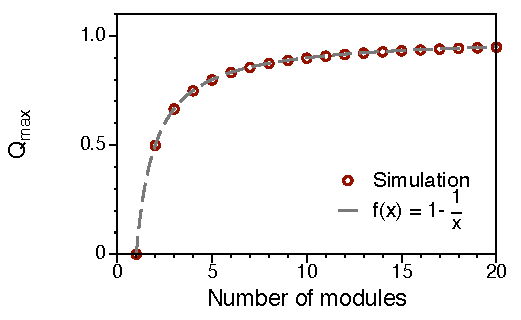
\includegraphics{Q_max.pdf}
\caption{Equation \eqref{eq:q_max} (grey dashed line) is in good agreement with numerical simulations (red circles).
In the simulations, modules are dense, directed subgraphs ($p_\mathrm{in}=0.5$) with $32$ nodes each.
Modules are connected on a ring so that the resulting graph is connected.
}
\label{fig:q_max}
\end{SCfigure}


\paragraph{Finite systems\color{Cayenne}{.}}
In finite systems, we get a minimum fraction of inter-module edges, when modules are connected to each other on a ring, each module having two nearest neighbors.
In this case we set  $e_{ij}= \frac{1}{n}(1-c)$ for $j=i+1$ and $j=i-1$ and all other elects are zero.
This yields
\begin{equation}\label{eq:ring_module_matrix}
e_{ij}=\left(\begin{array}{cccccc}
x_1 & \frac{1}{n}(1-c)&  & \hdots &  & 0 \\ 
\frac{1}{n}(1-c)& x_2 &\frac{1}{n}(1-c)&  &  &  \\
 & \frac{1}{n}(1-c) & \ddots & \ddots & & \\
\vdots &  & \ddots & \ddots & \ddots &\vdots \\
 & & & \ddots   &  x_{n-1} &\frac{1}{n}(1-c) \\
0 & &  & \hdots & \frac{1}{n}(1-c) & x_n
\end{array}
\right) .
\end{equation}
It follows immediately that $\sum _j e_{ij}=x_i+\frac{2(1-c)}{n}$, which is equivalent to \eqref{eq:sumeij} up to a factor 2.
Inserting this into equation \eqref{eq:modumatrix} gives a similar expression for modularity \eqref{eq:Qndim} as for the general case:
\begin{equation*}
Q=c-\sum _i x_i^2 - \frac{4(1-c)}{n} .
\end{equation*}
Since the relevant part for maximum finding is the quadratic term as in \eqref{eq:relevant_Q}, the results remain unchanged for modules along a chain.

\paragraph{Directed networks\color{Cayenne}{.}}
In analog to equation \eqref{eq:mod_undir} the modularity of directed networks can be written as \citep{Kao:2007}
\begin{equation}\label{eq:mod_directed}
Q=\sum _i e_{ii} - a_i ^{\text{in}} a_i ^{\text{out}}.
\end{equation}
where
\[
a_j ^\text{in}= \sum _i e_{ij} \hspace{1cm} \text{and} \hspace{1cm} a_i ^\text{out}= \sum _j e_{ij}.
\]
The structure of the inter-module edges takes the form of the matrix \eqref{eq:ring_module_matrix} and thus results do not differ either for the directed case.






%
%\bibliographystyle{apalike}
%\bibliography{/Users/lentz/Documents/GitHub_locals/Thesis/bibliography.bib}
%\end{document}
%

        \section*{List of abbreviations}
%\thispagestyle{plain}
\begin{acronym}[nnzzzzzzz] %5 l�ngste Abk�rzung ineckigen Klammern zur Ausrichtung
%\setlength{\itemsep}{-\parsep}
\acro{}[\color{Steel}{Networks}\color{Cayenne}{.}]{}
\acro{G}[$G$]{Network/Graph. A tuple $G=(V,E)$ of a set of nodes $V$ and a set of edges~$E$.}
\acro{N}[$N$]{Number of nodes of a network.}
\acro{m}[$m$]{Number of edges of a network.}
\acro{D}[$D$]{Network diameter.}
\acro{A}[$\mathbf{A}$]{Adjacency matrix.}
\acro{P}[$\mathbf{P}_{N-1}$]{Accessibility matrix.}
\acro{exists_path}[$u\rightarrow v$]{A path of arbitrary length exists between $u$ and $v$.}
\acro{k}[$k, k^+,k^-$]{Degree of a node, Out-degree, In-degree.}
\acro{gcc}[$G(S)CC$]{Giant (strongly) connected component.}
\acro{gwcc}[$GWCC$]{Giant weakly connected component.}
\acro{Q}[$Q$]{Modularity.}

\acro{}[]{}
\acro{}[\color{Steel}{Epidemic models}\color{Cayenne}{.}]{}
\acro{alpha}[$\alpha $]{Infection rate.}
\acro{gamma}[$\gamma $]{Recovery rate.}
\acro{rinfty}[$R_\infty $]{Outbreak size in SIR model.}

\acro{}[]{}
\acro{}[\color{Steel}{Temporal networks}\color{Cayenne}{.}]{}
\acro{tmpgraph}[$\mathcal{G}$]{Temporal network given by triple $\mathcal{G}=(V,\mathcal{E},T)$.}
\acro{Gstar}[$G^* (\mathcal{G}^*)$]{Transitive closure of a (temporal) network.}
\acro{exists_temp_path}[$u\rightsquigarrow v$]{A time respecting path exists between $u$ and $v$.}
\acro{t_horizon}[$\mathcal{H}_v$]{Horizon of node $v$.}
\acro{adjmatrixseq}[$\mathcal{A}$]{Sequence of adjacency matrices as a graph centric temporal network representation.}
\acro{nnz}[$\mathrm{nnz}(\mat{X})$]{Number of non zeros of a matrix $\mat{X}$.}
\acro{rho}[$\rho (\mathbf{X})$]{Density of a matrix $\mat{X}$, i.e. the number of occupied non zeros normalized by the number of all possible entries.}
\acro{pn}[$\mathcal{P}_n $]{Accessibility matrix of a temporal network over $n$ time steps.}
\acro{ranking}[$R(X)$]{Node ranking according to some measure $X$.}
\acro{infperiod}[$d$]{Infectious period.}
\acro{}[$r(v,d,t_0)$]{Range of a node for memory/infectious period $d$ and starting time $t_0$. Equivalent to outbreak size for simple compartment models.}
\end{acronym}

        \nocite{*}                
		% See the documentation or under
		% http://edoc.hu-berlin.de/e_autoren/latex/bedingung.php
		% for the list of the permitted styles.
        \bibliographystyle{apalike}
        \bibliography{bibliography}
        %\listoffigures
        %\listoftables    
        %% You can change this text, if needed.
\chapter*{Selbst"andigkeitserkl"arung}

Ich erkl"are, dass ich die vorliegende Arbeit selbst"andig und nur unter Verwendung der angegebenen Literatur und Hilfsmittel angefertigt habe.

\vspace{2\baselineskip}
\noindent Berlin, den 28.01.2008\hfill\authorfirstname \authorsurname    % Use our template or write your own.
        %%\markboth{List of publications}{List of publications}

\chapter*{List of publications}
%\thispagestyle{empty}
\begin{enumerate}
 \item \textbf{H. H. K. Lentz}, T. Selhorst and I. M. Sokolov\\
 \textit{Unfolding Accessibility provides a Macroscopic Approach to Temporal Networks}\\
  Physical Review Letters 110: 118701 (2013).

 \item M. Konschake, \textbf{H. H. K. Lentz}, F. J. Conraths, P. Hoevel and T. Selhorst\\
  \textit{On the Robustness of In- and Out-Components in a Temporal Network}\\
  PLoS ONE 8(2): e55223 (2013).

 \item \textbf{H. H. K. Lentz}, T. Selhorst and I. M. Sokolov\\
  \textit{Spread of infectious diseases in directed and modular metapopulation networks}\\
  Physical Review E 85: 066111 (2012).

  \item \textbf{H. H. K. Lentz},  M. Konschake, K. Teske, M. Kasper, B. Rother, R. Carmanns, B. Petersen, F. J. Conraths and T. Selhorst \\
   \textit{Trade communities and their spatial patterns in the German pork production network}\\
  Preventive Veterinary Medicine 98: 176--181 (2011).

  \item \textbf{H. Lentz},  M. Kasper and T. Selhorst \\
   \textit{Beschreibung des Handels mit Rindern in Deutschland mittels Netzwerkanalyse -- Ergebnisse von Voruntersuchungen}\\
  Berliner und M�nchener Tier�rztliche Wochenschrift 122: 193--198 (2009).

\end{enumerate}%\clearpage

%\vspace{2cm}
%\noindent Berlin, \today   \newline
%
%\par\hspace{8cm}  ( \authorfirstname \authorsurname)

        %\markboth{}{Curriculum Vitae}
\chapter*{Curriculum Vitae}

\begin{cv}{~}
  
\begin{cvlist}{\color{Steel}{Personal information}}
  \item Dipl.-Phys. Hartmut Lentz
    \item born in Siegen, October 23rd 1980\\
	Nationality: German
    \item[contact] Friedrich-Loeffler-Institute\\
    Institute for Epidemiology\\
    Seestr. 55\\
    106868 Wusterhausen, Germany
 % \item +49-(30)~2093-7750\\
   \item hartmut.lentz@fli.bund.de	

\end{cvlist}
%\vspace{0.1cm}
 % \noindent\hrulefill

  \begin{cvlist}{\color{Steel}{Education and job history}}
  \item[since 04/2008] Research assistant, Friedrich-Loeffler-Institute (Federal Research Institute for Animal Health), Working group Theoretical Epidemiology
   \item[since 04/2008] Ph.D. student, Humboldt-University of Berlin, Department of
Physics, Statistical Physics and nonlinear Dynamics, Topic: \emph{Spread of infectious diseases in complex networks}.
  \item[10/2007] Diploma in theoretical physics at Department of Physics, Technical University Berlin, Topic: \emph{Rotierende Wellenmuster in erregbaren Medien}, (graduated with honors).
  \item[10/2007--04/2008] Research assistant, Technical University Berlin
  \item[10/2001--10-2007] Physics study at Freie University Berlin and Technical University Berlin
  \item[06/2001] Abitur, Evangelisches Gymnasium Siegen
  \end{cvlist}

  \date{}
\end{cv}

%\vspace{1\baselineskip}
\noindent Berlin, \today   %\newline

\par\hspace{8cm}  ( \authorfirstname \authorsurname)

\end{document}
